\documentclass{report} % For LaTeX2e
\usepackage{iclr2024_conference,times}
% Optional math commands from https://github.com/goodfeli/dlbook_notation.
%%%%% NEW MATH DEFINITIONS %%%%%

\usepackage{amsmath,amsfonts,bm}

% Mark sections of captions for referring to divisions of figures
\newcommand{\figleft}{{\em (Left)}}
\newcommand{\figcenter}{{\em (Center)}}
\newcommand{\figright}{{\em (Right)}}
\newcommand{\figtop}{{\em (Top)}}
\newcommand{\figbottom}{{\em (Bottom)}}
\newcommand{\captiona}{{\em (a)}}
\newcommand{\captionb}{{\em (b)}}
\newcommand{\captionc}{{\em (c)}}
\newcommand{\captiond}{{\em (d)}}

% Highlight a newly defined term
\newcommand{\newterm}[1]{{\bf #1}}


% Figure reference, lower-case.
\def\figref#1{figure~\ref{#1}}
% Figure reference, capital. For start of sentence
\def\Figref#1{Figure~\ref{#1}}
\def\twofigref#1#2{figures \ref{#1} and \ref{#2}}
\def\quadfigref#1#2#3#4{figures \ref{#1}, \ref{#2}, \ref{#3} and \ref{#4}}
% Section reference, lower-case.
\def\secref#1{section~\ref{#1}}
% Section reference, capital.
\def\Secref#1{Section~\ref{#1}}
% Reference to two sections.
\def\twosecrefs#1#2{sections \ref{#1} and \ref{#2}}
% Reference to three sections.
\def\secrefs#1#2#3{sections \ref{#1}, \ref{#2} and \ref{#3}}
% Reference to an equation, lower-case.
\def\eqref#1{equation~\ref{#1}}
% Reference to an equation, upper case
\def\Eqref#1{Equation~\ref{#1}}
% A raw reference to an equation---avoid using if possible
\def\plaineqref#1{\ref{#1}}
% Reference to a chapter, lower-case.
\def\chapref#1{chapter~\ref{#1}}
% Reference to an equation, upper case.
\def\Chapref#1{Chapter~\ref{#1}}
% Reference to a range of chapters
\def\rangechapref#1#2{chapters\ref{#1}--\ref{#2}}
% Reference to an algorithm, lower-case.
\def\algref#1{algorithm~\ref{#1}}
% Reference to an algorithm, upper case.
\def\Algref#1{Algorithm~\ref{#1}}
\def\twoalgref#1#2{algorithms \ref{#1} and \ref{#2}}
\def\Twoalgref#1#2{Algorithms \ref{#1} and \ref{#2}}
% Reference to a part, lower case
\def\partref#1{part~\ref{#1}}
% Reference to a part, upper case
\def\Partref#1{Part~\ref{#1}}
\def\twopartref#1#2{parts \ref{#1} and \ref{#2}}

\def\ceil#1{\lceil #1 \rceil}
\def\floor#1{\lfloor #1 \rfloor}
\def\1{\bm{1}}
\newcommand{\train}{\mathcal{D}}
\newcommand{\valid}{\mathcal{D_{\mathrm{valid}}}}
\newcommand{\test}{\mathcal{D_{\mathrm{test}}}}

\def\eps{{\epsilon}}


% Random variables
\def\reta{{\textnormal{$\eta$}}}
\def\ra{{\textnormal{a}}}
\def\rb{{\textnormal{b}}}
\def\rc{{\textnormal{c}}}
\def\rd{{\textnormal{d}}}
\def\re{{\textnormal{e}}}
\def\rf{{\textnormal{f}}}
\def\rg{{\textnormal{g}}}
\def\rh{{\textnormal{h}}}
\def\ri{{\textnormal{i}}}
\def\rj{{\textnormal{j}}}
\def\rk{{\textnormal{k}}}
\def\rl{{\textnormal{l}}}
% rm is already a command, just don't name any random variables m
\def\rn{{\textnormal{n}}}
\def\ro{{\textnormal{o}}}
\def\rp{{\textnormal{p}}}
\def\rq{{\textnormal{q}}}
\def\rr{{\textnormal{r}}}
\def\rs{{\textnormal{s}}}
\def\rt{{\textnormal{t}}}
\def\ru{{\textnormal{u}}}
\def\rv{{\textnormal{v}}}
\def\rw{{\textnormal{w}}}
\def\rx{{\textnormal{x}}}
\def\ry{{\textnormal{y}}}
\def\rz{{\textnormal{z}}}

% Random vectors
\def\rvepsilon{{\mathbf{\epsilon}}}
\def\rvtheta{{\mathbf{\theta}}}
\def\rva{{\mathbf{a}}}
\def\rvb{{\mathbf{b}}}
\def\rvc{{\mathbf{c}}}
\def\rvd{{\mathbf{d}}}
\def\rve{{\mathbf{e}}}
\def\rvf{{\mathbf{f}}}
\def\rvg{{\mathbf{g}}}
\def\rvh{{\mathbf{h}}}
\def\rvu{{\mathbf{i}}}
\def\rvj{{\mathbf{j}}}
\def\rvk{{\mathbf{k}}}
\def\rvl{{\mathbf{l}}}
\def\rvm{{\mathbf{m}}}
\def\rvn{{\mathbf{n}}}
\def\rvo{{\mathbf{o}}}
\def\rvp{{\mathbf{p}}}
\def\rvq{{\mathbf{q}}}
\def\rvr{{\mathbf{r}}}
\def\rvs{{\mathbf{s}}}
\def\rvt{{\mathbf{t}}}
\def\rvu{{\mathbf{u}}}
\def\rvv{{\mathbf{v}}}
\def\rvw{{\mathbf{w}}}
\def\rvx{{\mathbf{x}}}
\def\rvy{{\mathbf{y}}}
\def\rvz{{\mathbf{z}}}

% Elements of random vectors
\def\erva{{\textnormal{a}}}
\def\ervb{{\textnormal{b}}}
\def\ervc{{\textnormal{c}}}
\def\ervd{{\textnormal{d}}}
\def\erve{{\textnormal{e}}}
\def\ervf{{\textnormal{f}}}
\def\ervg{{\textnormal{g}}}
\def\ervh{{\textnormal{h}}}
\def\ervi{{\textnormal{i}}}
\def\ervj{{\textnormal{j}}}
\def\ervk{{\textnormal{k}}}
\def\ervl{{\textnormal{l}}}
\def\ervm{{\textnormal{m}}}
\def\ervn{{\textnormal{n}}}
\def\ervo{{\textnormal{o}}}
\def\ervp{{\textnormal{p}}}
\def\ervq{{\textnormal{q}}}
\def\ervr{{\textnormal{r}}}
\def\ervs{{\textnormal{s}}}
\def\ervt{{\textnormal{t}}}
\def\ervu{{\textnormal{u}}}
\def\ervv{{\textnormal{v}}}
\def\ervw{{\textnormal{w}}}
\def\ervx{{\textnormal{x}}}
\def\ervy{{\textnormal{y}}}
\def\ervz{{\textnormal{z}}}

% Random matrices
\def\rmA{{\mathbf{A}}}
\def\rmB{{\mathbf{B}}}
\def\rmC{{\mathbf{C}}}
\def\rmD{{\mathbf{D}}}
\def\rmE{{\mathbf{E}}}
\def\rmF{{\mathbf{F}}}
\def\rmG{{\mathbf{G}}}
\def\rmH{{\mathbf{H}}}
\def\rmI{{\mathbf{I}}}
\def\rmJ{{\mathbf{J}}}
\def\rmK{{\mathbf{K}}}
\def\rmL{{\mathbf{L}}}
\def\rmM{{\mathbf{M}}}
\def\rmN{{\mathbf{N}}}
\def\rmO{{\mathbf{O}}}
\def\rmP{{\mathbf{P}}}
\def\rmQ{{\mathbf{Q}}}
\def\rmR{{\mathbf{R}}}
\def\rmS{{\mathbf{S}}}
\def\rmT{{\mathbf{T}}}
\def\rmU{{\mathbf{U}}}
\def\rmV{{\mathbf{V}}}
\def\rmW{{\mathbf{W}}}
\def\rmX{{\mathbf{X}}}
\def\rmY{{\mathbf{Y}}}
\def\rmZ{{\mathbf{Z}}}

% Elements of random matrices
\def\ermA{{\textnormal{A}}}
\def\ermB{{\textnormal{B}}}
\def\ermC{{\textnormal{C}}}
\def\ermD{{\textnormal{D}}}
\def\ermE{{\textnormal{E}}}
\def\ermF{{\textnormal{F}}}
\def\ermG{{\textnormal{G}}}
\def\ermH{{\textnormal{H}}}
\def\ermI{{\textnormal{I}}}
\def\ermJ{{\textnormal{J}}}
\def\ermK{{\textnormal{K}}}
\def\ermL{{\textnormal{L}}}
\def\ermM{{\textnormal{M}}}
\def\ermN{{\textnormal{N}}}
\def\ermO{{\textnormal{O}}}
\def\ermP{{\textnormal{P}}}
\def\ermQ{{\textnormal{Q}}}
\def\ermR{{\textnormal{R}}}
\def\ermS{{\textnormal{S}}}
\def\ermT{{\textnormal{T}}}
\def\ermU{{\textnormal{U}}}
\def\ermV{{\textnormal{V}}}
\def\ermW{{\textnormal{W}}}
\def\ermX{{\textnormal{X}}}
\def\ermY{{\textnormal{Y}}}
\def\ermZ{{\textnormal{Z}}}

% Vectors
\def\vzero{{\bm{0}}}
\def\vone{{\bm{1}}}
\def\vmu{{\bm{\mu}}}
\def\vtheta{{\bm{\theta}}}
\def\va{{\bm{a}}}
\def\vb{{\bm{b}}}
\def\vc{{\bm{c}}}
\def\vd{{\bm{d}}}
\def\ve{{\bm{e}}}
\def\vf{{\bm{f}}}
\def\vg{{\bm{g}}}
\def\vh{{\bm{h}}}
\def\vi{{\bm{i}}}
\def\vj{{\bm{j}}}
\def\vk{{\bm{k}}}
\def\vl{{\bm{l}}}
\def\vm{{\bm{m}}}
\def\vn{{\bm{n}}}
\def\vo{{\bm{o}}}
\def\vp{{\bm{p}}}
\def\vq{{\bm{q}}}
\def\vr{{\bm{r}}}
\def\vs{{\bm{s}}}
\def\vt{{\bm{t}}}
\def\vu{{\bm{u}}}
\def\vv{{\bm{v}}}
\def\vw{{\bm{w}}}
\def\vx{{\bm{x}}}
\def\vy{{\bm{y}}}
\def\vz{{\bm{z}}}

% Elements of vectors
\def\evalpha{{\alpha}}
\def\evbeta{{\beta}}
\def\evepsilon{{\epsilon}}
\def\evlambda{{\lambda}}
\def\evomega{{\omega}}
\def\evmu{{\mu}}
\def\evpsi{{\psi}}
\def\evsigma{{\sigma}}
\def\evtheta{{\theta}}
\def\eva{{a}}
\def\evb{{b}}
\def\evc{{c}}
\def\evd{{d}}
\def\eve{{e}}
\def\evf{{f}}
\def\evg{{g}}
\def\evh{{h}}
\def\evi{{i}}
\def\evj{{j}}
\def\evk{{k}}
\def\evl{{l}}
\def\evm{{m}}
\def\evn{{n}}
\def\evo{{o}}
\def\evp{{p}}
\def\evq{{q}}
\def\evr{{r}}
\def\evs{{s}}
\def\evt{{t}}
\def\evu{{u}}
\def\evv{{v}}
\def\evw{{w}}
\def\evx{{x}}
\def\evy{{y}}
\def\evz{{z}}

% Matrix
\def\mA{{\bm{A}}}
\def\mB{{\bm{B}}}
\def\mC{{\bm{C}}}
\def\mD{{\bm{D}}}
\def\mE{{\bm{E}}}
\def\mF{{\bm{F}}}
\def\mG{{\bm{G}}}
\def\mH{{\bm{H}}}
\def\mI{{\bm{I}}}
\def\mJ{{\bm{J}}}
\def\mK{{\bm{K}}}
\def\mL{{\bm{L}}}
\def\mM{{\bm{M}}}
\def\mN{{\bm{N}}}
\def\mO{{\bm{O}}}
\def\mP{{\bm{P}}}
\def\mQ{{\bm{Q}}}
\def\mR{{\bm{R}}}
\def\mS{{\bm{S}}}
\def\mT{{\bm{T}}}
\def\mU{{\bm{U}}}
\def\mV{{\bm{V}}}
\def\mW{{\bm{W}}}
\def\mX{{\bm{X}}}
\def\mY{{\bm{Y}}}
\def\mZ{{\bm{Z}}}
\def\mBeta{{\bm{\beta}}}
\def\mPhi{{\bm{\Phi}}}
\def\mLambda{{\bm{\Lambda}}}
\def\mSigma{{\bm{\Sigma}}}

% Tensor
\DeclareMathAlphabet{\mathsfit}{\encodingdefault}{\sfdefault}{m}{sl}
\SetMathAlphabet{\mathsfit}{bold}{\encodingdefault}{\sfdefault}{bx}{n}
\newcommand{\tens}[1]{\bm{\mathsfit{#1}}}
\def\tA{{\tens{A}}}
\def\tB{{\tens{B}}}
\def\tC{{\tens{C}}}
\def\tD{{\tens{D}}}
\def\tE{{\tens{E}}}
\def\tF{{\tens{F}}}
\def\tG{{\tens{G}}}
\def\tH{{\tens{H}}}
\def\tI{{\tens{I}}}
\def\tJ{{\tens{J}}}
\def\tK{{\tens{K}}}
\def\tL{{\tens{L}}}
\def\tM{{\tens{M}}}
\def\tN{{\tens{N}}}
\def\tO{{\tens{O}}}
\def\tP{{\tens{P}}}
\def\tQ{{\tens{Q}}}
\def\tR{{\tens{R}}}
\def\tS{{\tens{S}}}
\def\tT{{\tens{T}}}
\def\tU{{\tens{U}}}
\def\tV{{\tens{V}}}
\def\tW{{\tens{W}}}
\def\tX{{\tens{X}}}
\def\tY{{\tens{Y}}}
\def\tZ{{\tens{Z}}}


% Graph
\def\gA{{\mathcal{A}}}
\def\gB{{\mathcal{B}}}
\def\gC{{\mathcal{C}}}
\def\gD{{\mathcal{D}}}
\def\gE{{\mathcal{E}}}
\def\gF{{\mathcal{F}}}
\def\gG{{\mathcal{G}}}
\def\gH{{\mathcal{H}}}
\def\gI{{\mathcal{I}}}
\def\gJ{{\mathcal{J}}}
\def\gK{{\mathcal{K}}}
\def\gL{{\mathcal{L}}}
\def\gM{{\mathcal{M}}}
\def\gN{{\mathcal{N}}}
\def\gO{{\mathcal{O}}}
\def\gP{{\mathcal{P}}}
\def\gQ{{\mathcal{Q}}}
\def\gR{{\mathcal{R}}}
\def\gS{{\mathcal{S}}}
\def\gT{{\mathcal{T}}}
\def\gU{{\mathcal{U}}}
\def\gV{{\mathcal{V}}}
\def\gW{{\mathcal{W}}}
\def\gX{{\mathcal{X}}}
\def\gY{{\mathcal{Y}}}
\def\gZ{{\mathcal{Z}}}

% Sets
\def\sA{{\mathbb{A}}}
\def\sB{{\mathbb{B}}}
\def\sC{{\mathbb{C}}}
\def\sD{{\mathbb{D}}}
% Don't use a set called E, because this would be the same as our symbol
% for expectation.
\def\sF{{\mathbb{F}}}
\def\sG{{\mathbb{G}}}
\def\sH{{\mathbb{H}}}
\def\sI{{\mathbb{I}}}
\def\sJ{{\mathbb{J}}}
\def\sK{{\mathbb{K}}}
\def\sL{{\mathbb{L}}}
\def\sM{{\mathbb{M}}}
\def\sN{{\mathbb{N}}}
\def\sO{{\mathbb{O}}}
\def\sP{{\mathbb{P}}}
\def\sQ{{\mathbb{Q}}}
\def\sR{{\mathbb{R}}}
\def\sS{{\mathbb{S}}}
\def\sT{{\mathbb{T}}}
\def\sU{{\mathbb{U}}}
\def\sV{{\mathbb{V}}}
\def\sW{{\mathbb{W}}}
\def\sX{{\mathbb{X}}}
\def\sY{{\mathbb{Y}}}
\def\sZ{{\mathbb{Z}}}

% Entries of a matrix
\def\emLambda{{\Lambda}}
\def\emA{{A}}
\def\emB{{B}}
\def\emC{{C}}
\def\emD{{D}}
\def\emE{{E}}
\def\emF{{F}}
\def\emG{{G}}
\def\emH{{H}}
\def\emI{{I}}
\def\emJ{{J}}
\def\emK{{K}}
\def\emL{{L}}
\def\emM{{M}}
\def\emN{{N}}
\def\emO{{O}}
\def\emP{{P}}
\def\emQ{{Q}}
\def\emR{{R}}
\def\emS{{S}}
\def\emT{{T}}
\def\emU{{U}}
\def\emV{{V}}
\def\emW{{W}}
\def\emX{{X}}
\def\emY{{Y}}
\def\emZ{{Z}}
\def\emSigma{{\Sigma}}

% entries of a tensor
% Same font as tensor, without \bm wrapper
\newcommand{\etens}[1]{\mathsfit{#1}}
\def\etLambda{{\etens{\Lambda}}}
\def\etA{{\etens{A}}}
\def\etB{{\etens{B}}}
\def\etC{{\etens{C}}}
\def\etD{{\etens{D}}}
\def\etE{{\etens{E}}}
\def\etF{{\etens{F}}}
\def\etG{{\etens{G}}}
\def\etH{{\etens{H}}}
\def\etI{{\etens{I}}}
\def\etJ{{\etens{J}}}
\def\etK{{\etens{K}}}
\def\etL{{\etens{L}}}
\def\etM{{\etens{M}}}
\def\etN{{\etens{N}}}
\def\etO{{\etens{O}}}
\def\etP{{\etens{P}}}
\def\etQ{{\etens{Q}}}
\def\etR{{\etens{R}}}
\def\etS{{\etens{S}}}
\def\etT{{\etens{T}}}
\def\etU{{\etens{U}}}
\def\etV{{\etens{V}}}
\def\etW{{\etens{W}}}
\def\etX{{\etens{X}}}
\def\etY{{\etens{Y}}}
\def\etZ{{\etens{Z}}}

% The true underlying data generating distribution
\newcommand{\pdata}{p_{\rm{data}}}
% The empirical distribution defined by the training set
\newcommand{\ptrain}{\hat{p}_{\rm{data}}}
\newcommand{\Ptrain}{\hat{P}_{\rm{data}}}
% The model distribution
\newcommand{\pmodel}{p_{\rm{model}}}
\newcommand{\Pmodel}{P_{\rm{model}}}
\newcommand{\ptildemodel}{\tilde{p}_{\rm{model}}}
% Stochastic autoencoder distributions
\newcommand{\pencode}{p_{\rm{encoder}}}
\newcommand{\pdecode}{p_{\rm{decoder}}}
\newcommand{\precons}{p_{\rm{reconstruct}}}

\newcommand{\laplace}{\mathrm{Laplace}} % Laplace distribution

\newcommand{\E}{\mathbb{E}}
\newcommand{\Ls}{\mathcal{L}}
\newcommand{\R}{\mathbb{R}}
\newcommand{\emp}{\tilde{p}}
\newcommand{\lr}{\alpha}
\newcommand{\reg}{\lambda}
\newcommand{\rect}{\mathrm{rectifier}}
\newcommand{\softmax}{\mathrm{softmax}}
\newcommand{\sigmoid}{\sigma}
\newcommand{\softplus}{\zeta}
\newcommand{\KL}{D_{\mathrm{KL}}}
\newcommand{\Var}{\mathrm{Var}}
\newcommand{\standarderror}{\mathrm{SE}}
\newcommand{\Cov}{\mathrm{Cov}}
% Wolfram Mathworld says $L^2$ is for function spaces and $\ell^2$ is for vectors
% But then they seem to use $L^2$ for vectors throughout the site, and so does
% wikipedia.
\newcommand{\normlzero}{L^0}
\newcommand{\normlone}{L^1}
\newcommand{\normltwo}{L^2}
\newcommand{\normlp}{L^p}
\newcommand{\normmax}{L^\infty}

\newcommand{\parents}{Pa} % See usage in notation.tex. Chosen to match Daphne's book.

\DeclareMathOperator*{\argmax}{arg\,max}
\DeclareMathOperator*{\argmin}{arg\,min}

\DeclareMathOperator{\sign}{sign}
\DeclareMathOperator{\Tr}{Tr}
\let\ab\allowbreak

\usepackage{hyperref}
\usepackage{url}
%%%%%% Solution for URL line break %%%
\makeatletter
\g@addto@macro{\UrlBreaks}{\UrlOrds}
\makeatother
%%%%%%%%%%%%%%%%%%%%%%%%%%%
\newcommand{\fix}{\marginpar{FIX}}
\newcommand{\new}{\marginpar{NEW}}
\iclrfinalcopy % Uncomment for camera-ready version, but NOT for submission.

% Add PGFPlots and TikZ packages
\usepackage{pgfplots}
\usepgfplotslibrary{dateplot} % Only if you need date plots
\pgfplotsset{compat=newest} % Use this to always use the latest version available
\usepackage{tikz}
\usetikzlibrary{shapes.geometric, arrows} % For flow Charts
\usetikzlibrary{trees} % Loading the trees library for hierarchical diagrams
\usepackage[edges]{forest} % For drawing hierarchical trees
\usetikzlibrary{arrows.meta} % For custom arrow tips in trees

\usepackage{lscape}
\usepackage{amsmath}

\usepackage[acronym]{glossaries}
\makeglossaries
\newacronym{vit}{ViT}{Vision Transformer}
\newacronym{hiera}{Hiera}{Hierarchical Vision Transformer}
\newacronym{dino}{DINOv2}{Self-Distillation with no labels v2}
\newacronym{din}{DINO}{Self-Distillation with no labels}
\newacronym{ibot}{iBOT}{Image bert pre-training with online tokenizer}
\newacronym{daa}{DAA}{Drive and Act}
\newacronym{ir}{ImR}{Imbalanced Ratio}
\newacronym{nir}{NIR}{Near Infra Red}
\newacronym{kir}{KIR}{Kinect Infra Red}
\newacronym{rgb}{RGB}{Red Green Blue}
\newacronym{smote}{SMOTE}{Synthetic Minority Oversampling Technique}
\newacronym{svm}{SVM}{Support Vector Machines}
\newacronym{clara}{CLARA}{Clustering Large Applications}
\newacronym{dbscan}{DBSCAN}{Density-Based Spatial Clustering of Applications with Noise}
\newacronym{hdbscan}{HDBSCAN}{Hierarchical Density-Based Spatial Clustering of Applications with Noise}
\newacronym{scut}{SCUT}{Multi-class imbalanced data classification using SMOTE and cluster-based undersampling}
\newacronym{adas}{ADAS}{Advanced Driver Assistance Systems}
\newacronym{nhtsa}{NHTSA}{National Highway Traffic Safety Administration}
\newacronym{ssl}{SSL}{Self-Supervised learning}
\newacronym{swav}{SwAV}{Swapping Assignments between Views}
\newacronym{cnn}{CNN}{Convolutional Neural Networks}
\newacronym{dd}{DD}{Driver distraction}
\newacronym{rnn}{RNN}{Recurrent neural network}
\newacronym{mlp}{MLP}{Multi-layer perceptron}
\newacronym{sf}{SF}{State Farm Dataset}
\newacronym{inr}{IR}{Infra-Red}
%%%%%%%%%%%%%%%%%%%%%%%%%%%%%%%%%%%%%%%
\usepackage{algorithm}
\usepackage{algpseudocode}
%\usepackage{algorithmic}
\usepackage{float} % For the H placement specifier

%%%%%%%%%%%%%%%%%%%%%======== Code for the Title Page===%%%%%%%%%%%%%%%%%%%%
%%%%%%%%%%%%%%%%%%%%%%%%%%%%%%%%%%%%%%%%%%%%%%%%%%%%%%%%%%%%%%%%%%%%%%%%%%%%
%\usepackage{utf8}{inputenc}
\usepackage{xcolor}
\usepackage{geometry}
\usepackage{graphicx}
\usepackage{subcaption}
\begin{document}

\begin{titlepage}
    \centering
    
\includegraphics[width=0.3\textwidth]{UNIS-Dachmarke_rgb.jpg}\hfill
    
\includegraphics[width=0.3\textwidth]{iosb_logo.png}
    \vspace{1.0cm}
    
    % Thesis Title
    \Large{\textbf{Master Thesis}}\\
    \vspace{1.0cm}
    \Large{\textbf{Improved Driver Distraction Detection Using Self-Supervised Learning}}\\
    \vspace{1.0cm}
    
    % Author and Matriculation Number
    \normalsize{by}\\
    \vspace{0.5cm}
    \large{\textbf{Suraj Bhardwaj}}\\
    \normalsize{University of Siegen}\\
    \vspace{1.0cm}
    
    % Supervisors and Examiners
    \large{\textbf{Examiner 1: Prof. Dr. Michael Möller}}\\
    \normalsize{Head of Computer Vision Group}\\
    \normalsize{University of Siegen}\\
    \vspace{1.0cm}

    \large{\textbf{Examiner 2: Dr. Jovita Lukasik}}\\
    \normalsize{Post-Doctoral Researcher at Computer Vision Group}\\
    \normalsize{University of Siegen}\\
    \vspace{1.0cm}

    % Company Supervisor
    \large{\textbf{Additional Supervisor: David Lerch M.Sc.}}\\
    \normalsize{Perceptual User Interface Group}\\
    \normalsize{Fraunhofer IOSB, Karlsruhe}\\
    \vspace{1.5cm}
    
    % Thesis Submission Statement
    \normalsize{A Thesis Submitted to the Faculty of Electrical Engineering and Computer Science}\\
    \normalsize{In Partial Fulfillment of the Requirements for the Degree of Master of Science (M.Sc.)}\\
    \normalsize{\textbf{International Graduate Studies in Mechatronics}}\\
    \vfill
    \rule{\textwidth}{0.4pt}
    \normalsize{Universität Siegen}\\
    \normalsize{North Rhine-Westphalia, Germany}\\
    \normalsize{Date of Submission: 15 May 2024}\\
\end{titlepage}

% \section* is used for unnumbered sections like Declaration, Acknowledgments, and Abstract.
\chapter*{Declaration of Authorship}

I hereby confirm that this thesis and the work presented in it is entirely my own. Where I have
consulted the work of others this is always clearly stated. All statements taken literally from other
writings or referred to by analogy are marked and the source is always given. This paper has not yet
been submitted to another examination office, either in the same or similar form. 

\vspace{10mm} % Adjust the vertical space as needed

\noindent
\begin{tabular}{@{}lll@{}}
    Place, Date: & \textbf{Siegen, 15 May, 2024} & \hspace{1cm} Student's Signature: \hrulefill \\
\end{tabular}

\chapter*{Acknowledgments}
I am deeply grateful to my advisors, Prof. Dr. Michael Möller, Dr. Jovita Lukasik, and David Lerch M.Sc., for their invaluable guidance, enduring patience, and profound expertise throughout my research journey. Their insightful feedback and thoughtful recommendations were instrumental in shaping this thesis.

I also want to thank everyone at the Perceptual User Interface Department at Fraunhofer IOSB, Karlsruhe, for their support and for providing the tools and environment I needed for my work. My peers and colleagues at Fraunhofer IOSB also deserve profound acknowledgment for their friendship, engaging discussions during our regular student workshops, and the shared insights that significantly enriched my graduate experience.

I would also like to recognize the pioneering authors and researchers in my field whose foundational work has inspired and guided my research. Their significant contributions have illuminated my path and set a high standard for my work.

Finally, heartfelt gratitude goes to my family—my parents, Shri Sohan Singh and Smt. Jai Dei, and my niece Shivanshi. Their endless support and understanding through the demands of my academic pursuits have been a constant source of strength and motivation. Their love and encouragement have been the pillars of my strength and inspiration.

%Table of Contents
\newpage
\tableofcontents

%List of Figures
\newpage
\listoffigures

%List of Tables
\newpage
\listoftables

% Abbreviations
\newpage
\printglossary[type=\acronymtype]

\chapter*{Abstract}
This thesis investigates the binary classification task of classifying driver distraction using \gls{daa}~\citep{martin2019drive_and_act_2019_iccv} image datasets and vision transformer encoders that are pre-trained using Supervised and \gls{ssl} learning approaches respectively. The main focus is dealing with data imbalance, comparing the performance of vision transformer encoders pre-trained using supervised and \gls{ssl} approaches, and evaluating their ability to generalize across different views and modalities. In order to utilize the \gls{daa} video dataset, this thesis creates image datasets derived from the \gls{daa} dataset's videos. This study presents the `Clustered Feature Weighting' dataloading technique as a solution to the data imbalance issue in the image datasets derived from \gls{daa}~\citep{martin2019drive_and_act_2019_iccv} video dataset. This approach uses the HDBSCAN~\citep{HDBSCAN_algo_campello2013density} algorithm for unsupervised clustering of features extracted by a pre-trained vision transformer model. It also incorporates a weighted random sampler~\citep{pytorchweightedrandomsampler} to balance the training batches based on generated weights using unsupervised clustering. The results show that `Clustered Feature Weighting' successfully achieves a balanced class distribution in batches during data loading. Additionally, it shows signs of improvements in model performance on the Kinect Color \gls{daa} dataset~\citep{martin2019drive_and_act_2019_iccv}. Specifically, it increases the train balanced accuracy by 1.03\%, the validation balanced accuracy by 0.5\%, and the test balanced accuracy by 0.08\% compared to the traditional imbalanced dataloading method. Nevertheless, additional research is necessary to elucidate this technique's potential advantages and disadvantages for model training and generalization.

Furthermore, this thesis evaluates cross-view generalization across two different image views (right top and front top) and cross-modality generalization across two modalities (RGB and infrared) from \gls{daa} dataset on the driver distraction detection task. The SSL-based encoder consistently performed well in all permutations, especially when using infrared or grayscale imagery. Despite the problems in cross-view generalization, the findings affirm that \gls{ssl} based encoders have the potential to enhance the adaptability and robustness of driver distraction detection systems. The comparison between the SSL-based vision transformer~\citep{Vit_Paper_Dosovitskiy2020AnII} encoder, specifically the DINOv2~\citep{dinov2_oquab2023dinov2} based vit\_b\_14 encoder~\citep{dinov2_github}, and the supervised learning-based vit\_b\_16~\citep{vit_b_16_pytorch} encoder, demonstrated that the SSL-based model displayed remarkable feature extraction abilities, leading to significantly improved performance, especially in tasks that require generalization across grayscale or \gls{inr} image modality. On the \gls{kir} \gls{daa} cross-modality test dataset, the \gls{ssl}-based model showed a higher performance level on cross-modality generalization than the supervised learning-based model, with an improvement of up to 7.17\% . While the initial train balanced accuracies are satisfactory, underfitting highlights the urgent need for better hyperparameter optimization to fully use the model's potential. This thesis contributes significantly to automotive safety, demonstrating the feasibility and advantages of employing \gls{ssl}-based encoders for improving driver distraction detection.

\textbf{Keywords:} Self-Supervised Learning, Driver Distraction Detection, Cross-Modality Generalisation, Cross-View Generalisation, Drive and Act Image Dataset, Dataset Imbalance, Vision Transformer. 

%%%%%%%%%%%%%%%%%%%%%%%% Chapter 1: Introduction %%%%%%%%%%%%%%%%%%%%
%%%%%%%%%%%%%%%%%%%%%%%%%%%%%%%%%%%%%%%%%%%%%%%%%%%%%%%%%%%%%%%%%%%
\chapter{Introduction}
\label{chapter:introduction}
This chapter briefly introduces driver distraction detection. Why is it essential for the computer vision community, and how does it relate to real-world applications and problems? Furthermore, it includes the
central research questions guiding this thesis, along with a brief outline of the structure of this thesis.

\section{Introduction to Driver Distraction Detection}
Integrating artificial intelligence and advanced computing in the automotive industry has led to significant road safety and autonomous driving developments.~Although there have been significant technological improvements, most vehicles still rely on manual operation by the driver.~However, the primary cause for traffic accidents continues to be driver distraction, which includes participating in activities such as using mobile phones, texting, or conversing with passengers~\citep{bing_li_2022new, in_vehicle_cameras_9618784}.~\citet{WHO2023} investigated worldwide road traffic fatalities, advancements in safety legislation, and initiatives to decrease the number of deaths.~The data indicates a slight decline in annual fatalities caused by road traffic accidents, reaching 1.19 million~\footnote{\href{https://www.wbgalumni.org/event/data-for-action-on-road-safety-the-2023-global-status-report-on-road-safety/}{Data for Action on Road Safety: The 2023 Global Status Report on Road Safety}}.~However, it highlights the urgent requirement for significant measures to achieve the United Nations's target of reducing road traffic deaths and injuries by 50\% by 2030~\citep{WHO2023, Tanzania_Walugembe2020-ri}.~According to the~\citet{NHTSA2023}, distracted driving resulted in 3,308 deaths in 2022 in the USA.~The phenomenon of driver distraction displays notable variations in its development throughout its examination by researchers. Numerous seminal publications and review papers, such as~\citep{M1_regan2011driver, M2_young2007driver, in_vehicle_cameras_9618784, moslemi2021computer}, have thoroughly examined this phenomenon. 

According to~\citet{NHTSA2023}, 
\begin{quote}
    ``distracted driving is any activity that diverts attention from driving, including talking or texting on your phone, eating and drinking, talking to people in your vehicle, fiddling with the stereo, entertainment or navigation system — anything that takes your attention away from the task of safe driving."~\citep{NHTSA2023}
\end{quote}
This broad definition captures a variety of distraction types, including visual, manual, cognitive, and auditory distractions, as described in previous research works such as~\citet{moslemi2021computer, M1_regan2011driver, manual_li2020detection}.~For example, visual distractions can occur when drivers glance at passengers in the back seat, watch a multimedia screen, or look at objects placed on the passenger seat, thus diverting their focus from the road.~In contrast, cognitive distractions~\footnote{\href{https://www.drivesafeonline.org/traffic-school/cognitive-distractions/}{Cognitive Distractions While Driving: What You Need to Know}} arise when a driver is mentally absorbed in personal concerns or daydreams, even while visually monitoring the road~\citep{moslemi2021computer}.~As vehicles evolve towards higher levels of autonomy and reduce the driver's responsibilities, the likelihood of drivers engaging in distracting activities grows. This trend is expected to persist until vehicles reach full autonomy and no longer need any driver input~\citep{bing_li_2022new}.~This situation highlights the paradox where greater vehicle autonomy and minimal driver involvement do not necessarily equate to enhanced safety and reliability.

Moreover, the use of entertainment technology in vehicles has increased from its inception to the present.~According to the recent Allianz Distraction Study, such technologies significantly distract drivers, as evidenced in figure~\ref{fig:allaianz_dd_2023}~\citep{study_new_Allianz2023}.~This figure illustrates the rise in distracted driving activities from 2016 to 2022, paralleling technological advancements in the automotive sector.~At the same time, to mitigate these distractions, innovations in driver monitoring systems and their integration in the \gls{adas} play a crucial role by alerting distracted drivers, potentially reducing accident rates~\citep{moslemi2021computer}.

\begin{figure}[h]
\begin{center}
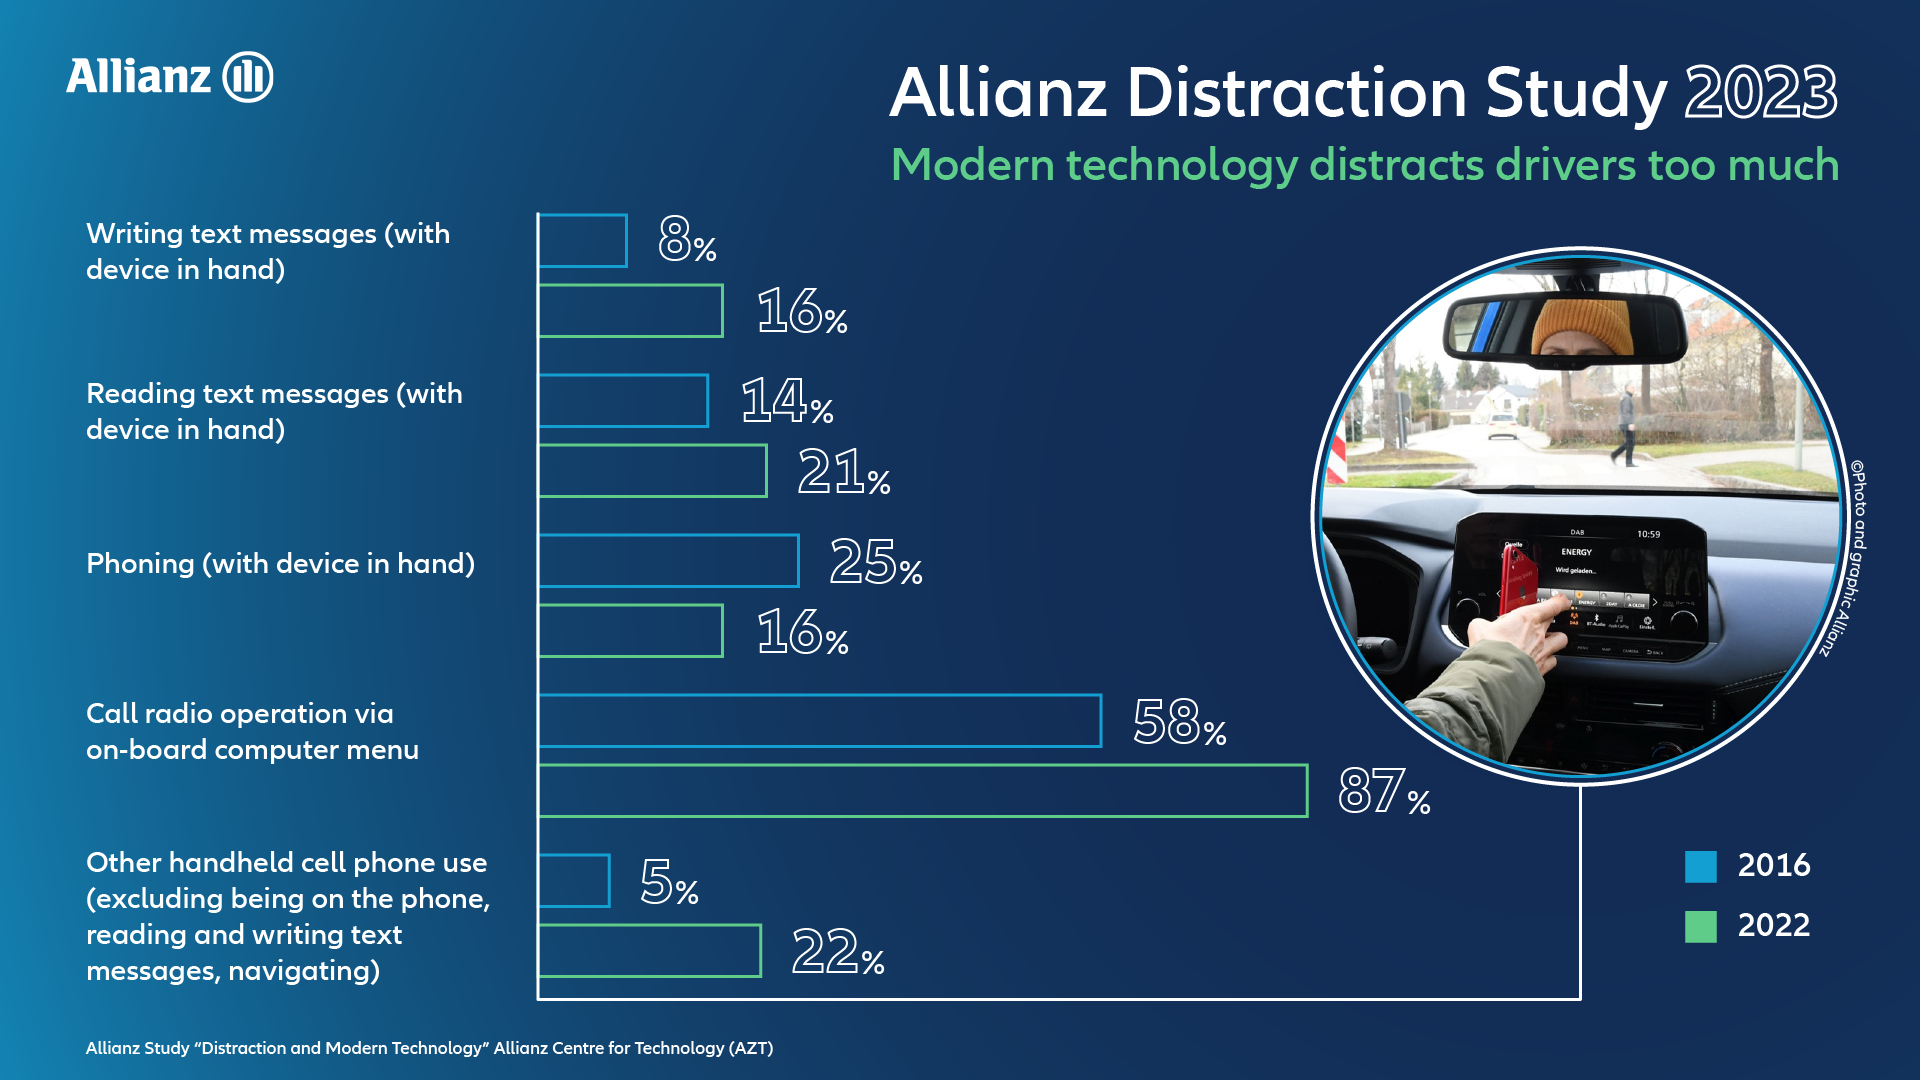
\includegraphics[width=0.8\textwidth]{Images_Thesis/Introduction_Related_Work/allianz-distraction-study-2023-technology-distracts-drivers.png}
\end{center}
\caption[Rise in distracted driving activities from 2016 to 2022]{Increase in instances of inattentive driving from 2016 to 2022. This figure illustrates the upward trend in various activities, such as reading text messages on a mobile phone while driving, from 2016 to 2022. These activities have played a role in the rise of distracted driving behavior. Source:~\citep{study_new_Allianz2023}}
\label{fig:allaianz_dd_2023}
\end{figure}

\section{Motivation}
Driver distraction stands as a significant cause of road accidents, necessitating rigorous research to foster a safer environment for road users~\citep{bing_li_2022new, in_vehicle_cameras_9618784, M1_regan2011driver, M2_young2007driver, moslemi2021computer}.~Such research aligns with the United Nations' 2030 goal to decrease road traffic fatalities and injuries substantially.~Traditionally, in computer vision, driver distraction detection has leveraged supervised learning algorithms, which depend on labeled data. However, acquiring this data is often expensive and labor-intensive.~Furthermore, supervised learning may not sufficiently generalize across diverse driving conditions, underscoring the need for unsupervised or self-supervised learning methods ~\citep{bing_li_2022new}.~Recent technological advances have equipped vehicles with various sensors and cameras, significantly enhancing the capability to monitor a broad spectrum of driver actions~\citet{in_vehicle_cameras_9618784, martin2019drive_and_act_2019_iccv}.~The \gls{daa} Dataset~\citep{martin2019drive_and_act_2019_iccv} presents a precious resource for pushing the boundaries of current research in driver activity recognition and distraction detection.~This dataset includes multiple data modalities, multi-view images, hierarchical labeling, and a detailed differentiation between various driver actions~\citep{martin2019drive_and_act_2019_iccv}.~These attributes combined establish it as an exceptional platform for extensive research and analysis. 

The primary objective of this research is to conduct a comprehensive exploration of the \gls{daa} Dataset~\citep{martin2019drive_and_act_2019_iccv} aimed at enhancing our understanding and detection of driver distractions.~This study engages in meticulous experimentation and analysis to assess the efficacy of using \gls{rgb} (color) and \gls{inr} (Gray Scale) imaging modalities from the \gls{daa} video dataset~\citep{martin2019drive_and_act_2019_iccv}.~A focal point of this research is extracting and creating image datasets and addressing dataset imbalances.

In advancing the field of driver distraction detection, this thesis utilizes advanced pre-trained vision transformer encoders.~It explores their application across different image modalities and views, testing their adaptability and generalizability.~The comparative analysis includes an encoder trained using a supervised learning technique and the one developed through \gls{ssl} framework DINOv2~\citep{dinov2_oquab2023dinov2}.~The sole purpose of this analysis is to highlight the performance of encoders trained using different techniques like supervised and \gls{ssl} on driver distraction detection and to evaluate the impact of various data modalities and image views on the accuracy and generalization of distraction detection.

Ultimately, this thesis aims to enhance driving safety, aligning with global safety objectives significantly.

\section{Research Questions}
\label{section:research_questions}
This thesis embarks on an exploration guided by these essential research questions:
\begin{itemize}
    \item \textbf{Practical Challenges:}~How can the issue of data imbalance in the \gls{daa} dataset~\citep{martin2019drive_and_act_2019_iccv} be addressed?~Is it possible to employ unsupervised learning techniques for this purpose, and if so, how can they be effectively implemented?
    
    \item \textbf{Effectiveness of \gls{ssl} Models:}~What are the benefits and drawbacks of using vision transformer encoders pretrained using \gls{ssl} based approaches, such as \gls{dino}~\citep{dinov2_oquab2023dinov2} over supervised learning based encoder, for detecting driver distraction?
    
    \item \textbf{Generalization Capabilities:}~How do different image views, such as the right top view and the front top view in the \gls{daa} dataset~\citep{martin2019drive_and_act_2019_iccv}, impact the detection of driver detection using computer vision?~Additionally, does a vision transformer~\citep{Vit_Paper_Dosovitskiy2020AnII} encoder pre-trained using a self-supervised learning approach maintain consistent performance on driver distraction detection tasks or generalize well across different views at hand?
    
    \item \textbf{Data Modality Impact:}~What are the impacts of varying data modalities, such as \gls{rgb} and \gls{inr} images, on detecting driver distractions? Furthermore, does the vision transformer encoder pre-trained using the self-supervised learning approach DINOv2~\citep{dinov2_oquab2023dinov2} demonstrate effective generalization across these modalities?
\end{itemize}

\section{Brief Outline of the Thesis}
The structure of the rest of the thesis is as follows:
\begin{itemize}
    \item \textbf{Chapter 2: Related Work} - A thorough literature review examines existing methods and technologies relevant to driver distraction detection.~This chapter highlights the limitations of conventional supervised learning approaches and highlights the necessity for innovative unsupervised or self-supervised learning models.~It also highlights the practical challenges with \gls{daa} dataset and identifies the research gaps this thesis aims to address.
    
    \item \textbf{Chapter 3: Background} - This chapter details the essential methodologies employed in this thesis.~It explains the working principle of the HDBSCAN~\citep{HDBSCAN_algo_campello2013density} clustering algorithm and vision transformer~\cite{Vit_Paper_Dosovitskiy2020AnII} and introduces relevant mathematical functions and terminology necessary for subsequent discussions.~Furthermore, it explains the self-supervised learning-based framework DINO~\citep{dino_caron2021emerging}, as well as the DINOv2 framework~\citep{dinov2_oquab2023dinov2}.
    
    \item \textbf{Chapter 4: Proposed Methods} - This chapter provides a comprehensive explanation of the innovative dataloader implementation, as well as a methodology to compare it with the traditional dataloader. This chapter also provides descriptions of the methodologies used in supervised learning-based encoder experiments and self-supervised learning-based encoder experiments.~Furthermore, this chapter discusses the theoretical foundations of the selected methods and explains their relevance in addressing the research goals outlined in the section~\ref{section:research_questions}.
    
    \item \textbf{Chapter 5: Experiments and Results} - This section delves into the experimental setup, highlighting the datasets utilized and the hyperparameter choices made. It also presents the implementation and results of the previously outlined methodologies across all experiments, offering a comprehensive analysis of the findings. Moreover, it specifically addresses the research questions posed in section~\ref{section:research_questions}.
    
    \item \textbf{Chapter 6: Conclusions and Future Work} - Concluding the thesis, this section integrates the findings, and identifies potential areas for future research to foster continued advancements in the field.
\end{itemize}

%% Please note that we have introduced automatic line number generation
%% into the style file for \LaTeXe. This is to help reviewers
%% refer to specific lines of the paper when they make their comments. Please do
%% NOT refer to these line numbers in your paper as they will be removed from the
%% style file for the final version of accepted papers.

%\begin{center}
%   \url{http://www.iclr.cc/}
%\end{center}
% The formatting instructions contained in these style files are summarized in
% sections \ref{gen_inst}, \ref{headings}, and \ref{others} below.
%%%%%%%%%%%%%%%%%%%%%%%% Chapter 2: Related Work %%%%%%%%%%%%%%%%%%%%
%%%%%%%%%%%%%%%%%%%%%%%%%%%%%%%%%%%%%%%%%%%%%%%%%%%%%%%%%%%%%%%%%%%
\chapter{Related Work}
\label{chapter:related_work}
Continuing from the previous chapter, where we discussed this thesis's goals and their relevance to real-world applications, this chapter provides a detailed literature review of existing distraction detection methods in computer vision. It highlights the limitations of traditional supervised learning methods and underscores the need for innovative unsupervised or self-supervised learning models. Additionally, this chapter addresses research gaps and discusses practical issues associated with the \gls{daa} dataset.

%%%%%%%%%%%%% My Text Here %%%%%%%%%%
\section{Supervised Learning Based Methods}
Supervised learning is a prevalent approach in detecting driver distractions, leveraging annotated datasets to
train models to recognize distraction patterns. In the research work on driver distraction detection,~\citet{58_MIM_zhang2016apply} applied and compared the performance of \gls{svm}~\citep{SVM_cortes1995support} and \gls{cnn}~\citep{CNN_o2015introduction} algorithms using the \gls{sf}~\citep{statefarm2016} dataset which contains 10 classes for driver distraction detection. For \gls{svm}~\citep{SVM_cortes1995support},~\citet{58_MIM_zhang2016apply} utilized a Support Vector Classifier (SVC) model employing a one-vs-one scheme to handle multi-class classification. The \gls{cnn}~\citep{CNN_o2015introduction} approach involved three models: a simple \gls{cnn} based on the MNIST~\citep{MNIST_dataset_deng2012mnist} digit classification task, a transfer learning model leveraging the pre-trained VGG-16~\citep{VGG_16_simonyan2014very}, and a modified VGG model (VGG-GAP)~\citep{VGG_GAP_zhou2016learning} with global average pooling layers. The \gls{cnn} models outperformed the \gls{svm}, with the simple \gls{cnn}~\citep{CNN_o2015introduction} achieving an accuracy of 63.3\%, VGG-16~\citep{VGG_16_simonyan2014very} reaching 90.2\%, and VGG-GAP~\citep{VGG_GAP_zhou2016learning} achieving 91.3\%. The ensemble of VGG-16 and VGG-GAP demonstrated superior performance with an accuracy of 92.6\%~\citep{58_MIM_zhang2016apply}.

\citet{mim_55_alexnet_okon2017detecting} used the AlexNet~\citep{Alexnet_krizhevsky2012imagenet} architecture as a baseline model (Model A) for the driver distraction detection task on the \gls{sf} dataset~\citep{statefarm2016}. AlexNet~\citep{Alexnet_krizhevsky2012imagenet}  was chosen because of its demonstrated capacity to classify a variety of items, including phones and driver's hands, which are useful for detecting distracted driving behaviors. Model A achieved a classification test accuracy of 96.8\% on the \gls{sf} dataset~\citep{statefarm2016}. To increase the model's performance even more,~\citet{mim_55_alexnet_okon2017detecting} introduced an upgraded version (Model B) that incorporated triplet loss. This approach considerably improved classification accuracy, with Model B scoring 98.7\% on the \gls{sf} dataset\citep{mim_55_alexnet_okon2017detecting}.

\citet{59_MIM_Sup_majdi2018drive} proposed `Drive-Net' a supervised learning method that combines a \gls{cnn}~\citep{CNN_o2015introduction} with a random decision forest~\citep{Random_decision_forest_ho1995random} for driver distraction detection.~Drive-Net's~\citep{59_MIM_Sup_majdi2018drive} \gls{cnn} architecture is derived from a modified U-Net~\citep{U_net_ronneberger2015u} model, where the up-convolution layers and the last two down-sampling layers are replaced by a 1x1 convolution layer. The random decision forest~\citep{Random_forest_ferns_bosch2007image} in Drive-Net comprises multiple decision trees trained with randomized data subsets and optimized by maximizing information gain at each node. Drive-Net was evaluated against a \gls{rnn}~\citep{RNN_Used_Object_Rec_liang2015recurrent} and a \gls{mlp}~\citep{MLP_classifier_haykin2009neural} using the \gls{sf} dataset~\citep{statefarm2016}. Utilizing k=5 in k-fold cross-validation~\citep{cross_val_hastie2009elements}, Drive-Net achieved a 95\% classification accuracy, outperforming \gls{rnn} and \gls{mlp} classifiers, which scored 91.7\% and 82\%, respectively\citep{59_MIM_Sup_majdi2018drive}.

\citet{60_MIM_Sup_janet2020real} used \gls{cnn} to detect driver distractions using the \gls{sf} dataset. \citet{60_MIM_Sup_janet2020real} tested three models: a vanilla CNN, a vanilla CNN with data augmentation, and a \gls{cnn} with transfer learning. The vanilla CNN, which included three convolutional layers and three dense layers, had the highest accuracy of 97.66\%. The data-augmented vanilla CNN achieved an accuracy of 97.05\%, while the transfer learning model, which used VGG~\citep{VGG_16_simonyan2014very} and MobileNet~\citep{MobileNet_howard2017mobilenets} to shorten training time, achieved 71.72\%~\citep{60_MIM_Sup_janet2020real}.

\citet{61_MIM_Sup_dhakate2020distracted} introduced an ensemble of \gls{cnn} for driver distraction detection on the \gls{sf} dataset. The proposed approach entails training several \gls{cnn} models, including VGG-16, VGG-19~\citep{VGG_16_simonyan2014very}, InceptionV3~\citep{Inception_V3_szegedy2016rethinking}, ResNet-50~\citep{Resnet_50_he2016deep}, and Xception~\citep{Xception_chollet2017xception}, by eliminating their final layers to extract feature vectors. These vectors are then combined using a stacking ensemble technique to train a meta-classifier \gls{cnn}, achieving a classification accuracy of 97\%. The ensemble stacking technique blends the outputs of different base-level models, enhancing overall prediction accuracy. The best-performing ensemble model in \citep{61_MIM_Sup_dhakate2020distracted} , a combination of ResNet-50~\citep{Resnet_50_he2016deep}, Xception~\citep{Xception_chollet2017xception}, InceptionV3~\citep{Inception_V3_szegedy2016rethinking}, and VGG-19~\citep{VGG_16_simonyan2014very}, achieved 97\% accuracy, significantly outperforming a simpler ensemble model of Xception and InceptionV3, which achieved 73\% accuracy on the \gls{sf} dataset~\citep{61_MIM_Sup_dhakate2020distracted}.

\citet{56_MIM_HCF_9113267} developed a hybrid \gls{cnn} framework (HCF) aimed at detecting distracted driving behaviors on the \gls{sf} dataset. This framework integrated three pretrained models—ResNet50, Inception V3, and Xception—to extract comprehensive behavior features through cooperative transfer learning. The extracted features were integrated into a detailed feature set, which is then classified using fully connected layers.~\citet{56_MIM_HCF_9113267} employed an improved dropout algorithm to prevent overfitting and class activation mapping (CAM) to highlight key features. HCF framework achieved a classification accuracy of 96.74\% on the \gls{sf} dataset~\citep{56_MIM_HCF_9113267}. 

\citet{26_MIM_qin2021distracted} proposed D-HCNN, a \gls{cnn} with decreasing filter fize, for real-time distracted driving detection. \citet{26_MIM_qin2021distracted} focused on building a highly accurate, fast, and low parameter count based model. As a result,  D-HCNN uses only 0.76M parameters, and incorporates Histogram of Oriented Gradients (HOG)~\citep{HOG_dalal2005histograms} images, L2 regularization, dropout, and batch normalization. D-HCNN begins with large convolution filters to capture broad features and progressively reduces filter sizes for detailed feature extraction. The D-HCNN architecture includes four convolutional layers with decreasing filter sizes (12x12, 9x9, 6x6, 3x3), followed by ReLU~\citep{ReLU_DBLP:journals/corr/abs-1803-08375}, max-pooling~\citep{Max_Pooling_32}, batch normalization~\citep{Batch_Norm_DBLP:journals/corr/IoffeS15}, and dropout layers~\citep{dropout_srivastava2014dropout}, concluding with global average pooling~\citep{Global_avg_pooling_Lin2013NetworkIN} and softmax classification. \citet{26_MIM_qin2021distracted} converts RGB images to grayscale in the proposed D-HCNN model to mitigate lighting effects and reduce computation. It also employs zero-mean normalization and random cropping for data augmentation. Evaluated on the AUC Distracted Driver (AUCD2)~\citep{AUC_D3_dataset_abouelnaga2017real} and \gls{sf} datasets, D-HCNN achieved accuracies of 95.59\% and 99.87\%, respectively.

\citet{57_MIM_octave_CNN_9457109} introduced ``OLCMNet" a lightweight octave-like \gls{cnn}~\citep{octave_convolution_chen2019drop}, for detecting driver distraction.~\citet{57_MIM_octave_CNN_9457109} developed an octave-like convolution mixed block (OLCM) to efficiently process feature maps by separating them into low and high-frequency branches, followed by global information fusion through squeeze-and-excitation (SE)~\citep{SE_module_hu2018squeeze} modules.~The architecture consists of a head, feature extraction, and final stage, with the OLCM block reducing spatial redundancy and improving computational efficiency. ~\citet{57_MIM_octave_CNN_9457109} also created Lilong Distracted Driving Behavior (LDDB) dataset, containing 267,378 annotated images from on-road experiments. The proposed OLCMNet achieved 95.98\% accuracy when evaluated on the (LDDB) dataset and 89.53\% accuracy on the \gls{sf} dataset.~\citet{57_MIM_octave_CNN_9457109} highlighted that squeeze-and-excitation module~\citep{SE_module_hu2018squeeze} in the final stage enhanced information exchange between layers, resulting in higher classification accuracy.

The aforementioned research demonstrates the effectiveness of various supervised learning techniques and \gls{cnn} structures, including simple CNNs, transfer learning models, hybrid frameworks, and ensemble methods, in accurately detecting driver distractions on conventional datasets such as \gls{sf} and AUCD2~\citep{AUC_D3_dataset_abouelnaga2017real}. However, there are notable drawbacks linked to using supervised learning methods for the driver distraction detection task. 

\paragraph{Drawbacks of Supervised Learning Based Methods:}
The aforementioned research typically employs supervised \gls{cnn} models, which demand large amounts of labeled data for training. This labeling process is resource-intensive, making it difficult to implement such models in real-world applications. Also these methods rely on manually selected features combined with classifiers and suffer from non-universality and poor adaptability to diverse driving scenarios~\citep{bing_li_2022new, masked_image_modeling_dd_zhang2023novel}. The reliance on supervised frameworks, such as \gls{cnn}s, limits their ability to generalize across different driving scenarios due to the need for extensive reliable labeled data. Furthermore, while \gls{cnn}s are effective at learning local image features, they struggle with capturing the global context necessary for accurately detecting driver distractions in complex real-world environments~\citep{bing_li_2022new, masked_image_modeling_dd_zhang2023novel}. This narrow focus hinders their overall perceptual ability, which is essential for comprehending spatial relationships and high-level semantic information in driving scenes~\citep{masked_image_modeling_dd_zhang2023novel}. Additionally, the intricate nature of real-world driving situations complicates the accurate labeling of data, thereby escalating the difficulty and cost of dataset creation . Overall, these factors contribute to the limited generalization performance and weak iterative ability of current supervised CNN-based models~\citep{masked_image_modeling_dd_zhang2023novel}.

\section{Unsupervised and Self-Supervised Learning Based Methods}
This section presents solutions to the constraints of methods that rely on supervised learning and highlights the advantages of unsupervised and self-supervised learning techniques for detecting driver distraction.~\citet{bing_li_2022new} introduced a novel unsupervised deep learning technique called ``Unsupervised deep learning framework (UDL)" to address the constraints of current supervised methods in driver distraction detection. UDL harnesses vast quantities of unannotated data, hence increasing its applicability for industrial purposes~\citep{bing_li_2022new}. In order to enhance generalization, the Simsiam~\citep{Simsiam_chen2021exploring_stop_grad} unsupervised model was updated.~\citet{bing_li_2022new} incorporated a \gls{mlp} design influenced by RepMLP~\citep{RepMLP_ding2021repmlp}. This architecture combines both local and global feature extraction methods. This method improved the model's capacity to adjust to different driving situations.~\citet{bing_li_2022new} also incorporated residuals into the projection head as a means of mitigating feature deterioration in multilayer architectures. This enhances the process of extracting deep features and improves the precision of detecting distractions~\citep{bing_li_2022new}. A novel loss function was developed by integrating comparative learning~\citep{comparative_learning_chen2020simple} with the stop-gradient~\citep{Simsiam_chen2021exploring_stop_grad} technique. This loss function aims to improve the model's ability to learn robust features, hence boosting its generalization performance~\citep{bing_li_2022new}. The UDL technique underwent testing using the \gls{sf} dataset, and it achieved a notable accuracy rate of 97.38\% during linear evaluation. This performance surpassed that of other unsupervised models like SimSiam with ResNet50 backbone (86.29\%), and SimCLR~\citep{Simsiam_chen2021exploring_stop_grad} with ResNet50 (94.32\%) during linear evaluation~\citep{bing_li_2022new}. The UDL method offers a substantial improvement in identifying driver distraction by utilizing unsupervised learning. The approach optimizes the utilization of unlabeled data, enhances the process of extracting features, and exhibits exceptional performance and flexibility, effectively overcoming the constraints of supervised models~\citep{bing_li_2022new}.

Self-supervised models outperform supervised models in capturing high-level semantic information by focusing feature attention on important discrimination regions more efficiently~\citep{masked_image_modeling_dd_zhang2023novel}.~\citet{masked_image_modeling_dd_zhang2023novel} developed SL-DDBD, a self-supervised learning method for detecting driver distraction behavior. The method uses a masked image modeling framework to reduce labeling costs.~\citet{masked_image_modeling_dd_zhang2023novel} reconfigured the Swin Transformer~\citep{swin_transformer_paper_liu2021swin} encoder, and utilized data augmentation strategies and optimal random masking strategies in the SL-DDBD method. The method achieved 99.60\% accuracy on the \gls{sf} dataset~\citep{statefarm2016}, with pre-training and transfer learning for downstream driver distraction task.

Despite the numerous advantages of unsupervised learning and self-supervised learning over supervised learning, there have been limited research that have applied these methods for identifying driver distraction. Therefore, it is imperative to transition towards these learning paradigms in order to develop more resilient, dependable, and effective systems for detecting driver distraction.

\section{Different Data Modalities}
The success of machine learning models is significantly determined by the quality and characteristics of the data. Similarly, the reliability of driver distraction detection systems relies on the integration of several data modalities and their relationship, as well as their collective impact on overall effectiveness~\citep{RA_2023_dd_article}. Several academics have examined driver distraction detection using various perspectives of data modalities. Physiological data offer direct insights into the driver's condition and correlate strongly with distraction levels~\citep{RA_52_reimer2011impact,RA_89_son2021effects, RA_133_almahasneh2014deep, RA_134_lin2011eeg}. Visual data, crucial for the success of supervised algorithms, includes tracking eye movement and body posture. The precision of these models depends on the accuracy of data collection methods like electroencephalography (EEG), which require adjustments to reduce interference from external physiological activities~\citep{RA_144_lin2005eeg, RA_145_lakshmi2014survey}.~\citet{RA_2023_dd_article} provided an overview of various types of data used in driver distraction detection research. These include physiological data (such as brain activity, breathing rate, skin conductivity and heart rate) and visual data (such as eye movement, body movement, and head movement). \citet{RA_2023_dd_article} emphasized the importance of combining different data modalities to improve the accuracy and reliability of driver distraction detection models. 

\section{Role of Drive and Act Dataset:}
The availability and quality of datasets are critical in exploring solutions to driver distraction.~\citet{moslemi2021computer} summarized the research on driver distraction based on key datasets such as the ~\gls{sf}~\citep{statefarm2016}, and the American University in Cairo (AUC)~\citep{AUC_D3_dataset_abouelnaga2017real} datasets. These datasets vary in characteristics, presenting challenges like differing lighting conditions, camera angles, and the level of detail in recorded actions, which can affect the models' general applicability and effectiveness~\citep{moslemi2021computer}.

The~\gls{daa} dataset, as detailed in~\citep{martin2019drive_and_act_2019_iccv}, is an innovative resource carefully assembled to advance research in driver behavior detection during both manual and automated driving scenarios. This extensive dataset comprises over 9.6 million frames, encapsulating 12 hours of video footage. It systematically captures a broad spectrum of distracting behaviors by integrating diverse types of data such as color, depth, infrared, and 3D body pose information, as illustrated in Figure~\ref{fig:driveandact_salient_features}. Data collection employed six different camera angles, utilizing five Near-Infrared (NIR) cameras and one Kinect v2 camera, the latter used for capturing color images in three channels (RGB), as well as infrared and depth data. The NIR cameras in the dataset operate at a resolution of 1280 x 1024 pixels and a frame rate of 30 Hz, while the Microsoft Kinect camera records color videos at 950 x 540 pixels with a 15 Hz frame rate and captures infrared and depth data at 512 x 424 pixels at 30 Hz~\citep{martin2019drive_and_act_2019_iccv}. The dataset was acquired using a stationary driving simulator, which was selected to ensure participant safety and effectively simulate various driving scenarios. This controlled environment mitigates risks associated with real-world driving and allows for consistent data collection across diverse conditions. Furthermore, the dataset benefits from including a heterogeneous group of participants varying in body size, driving experience, and familiarity with car automation technologies~\citep{martin2019drive_and_act_2019_iccv}. This diversity enriches the dataset, capturing various driving behaviors and styles. The \gls{daa} dataset is randomly segmented into three groups based on the identity of the driver. This splitting approach ensures that data from the same individual is not present across multiple splits, preventing potential overfitting or data leakage~\citet{martin2019drive_and_act_2019_iccv}. Specifically,~\citet{martin2019drive_and_act_2019_iccv} state:

\begin{quote}``for each split, we use the data of ten different identities for training, two for validation, and three for testing." ~\citep{martin2019drive_and_act_2019_iccv}   
\end{quote}

By splitting the dataset in this manner, the authors aim to create a challenging benchmark that evaluates the generalization capabilities of models trained on the \gls{daa} dataset. The three distinct splits allow for proper training, validation, and testing procedures, enabling robust evaluation of driver behavior recognition and driver distraction detection algorithms on unseen data from new individuals not present in the training set.

The \gls{daa} dataset uses a three-level hierarchy to detail driver interactions as depicted in the figures~\ref{fig:driveandact_activities} and~\ref{fig:driveandact_salient_features}, providing a comprehensive framework for analyzing driver behavior under both manual and automated conditions. At the highest level of the hierarchy are the tasks, which outline broad scenarios that participants encountered during the data collection. These tasks, such as entering the car and switching to autonomous driving, set the context for the actions and are vital for simulating realistic driving environments. They also include potentially distracting situations anticipated with increased automation, like using a laptop. The mid-level in this hierarchy consists of mid-level actions. These are fine-grained activities that further break down the tasks into more specific behaviors but still maintain a clear semantic meaning. For example, while a task might involve using a laptop, the mid-level actions detail the individual activities involved, such as typing or browsing. At the most detailed level are atomic action units, which describe basic interactions within the driving environment without long-term semantic implications. These units are defined by a combination of action, object, and location—such as `reaching for a jacket in the left backseat'. This level provides the fundamental building blocks of driver behavior, capturing the minute detail of every interaction~\citep{martin2019drive_and_act_2019_iccv}.

This hierarchical labeling not only enhances the granularity of behavioral analysis but also supports the development of sophisticated models that can predict and interpret diverse driving behaviors in real-time. By examining these interactions across different levels of abstraction, researchers can gain deeper insights into how drivers respond to various driving conditions and tasks, contributing to safer automotive technologies.

\begin{figure}[htbp]
\begin{center}
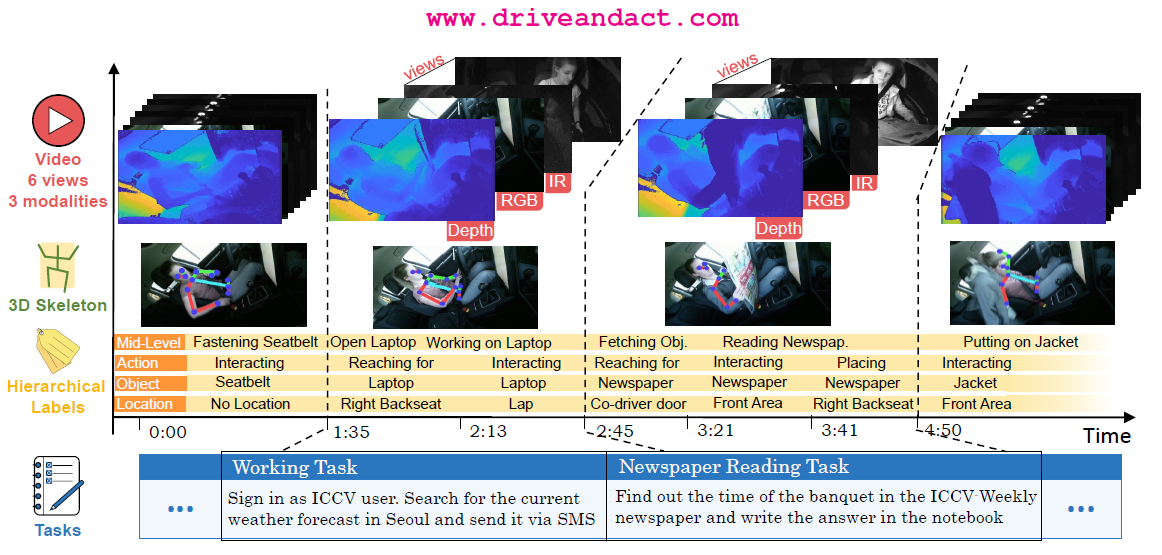
\includegraphics[width=0.8\textwidth]{Images_Thesis/daa_images/Capture_daa_thesis.PNG}
\end{center}
\caption[Drive and act dataset with its salient features.]{Drive and act dataset with its salient features. On the y-axis different modalities in the drive and act dataset can be seen along with the hierarchical labeling scheme guided by the 12 predefined tasks that each participant is subjected to perform in order to do the desired data collection. On the x-axis the time stamps along with the tasks that each participant in performing with respect to the time is shown. This figure also depicts the hierarchy in labeling where mid-level activities are fine grained activities and action, object and location combined together forms a complete driver action. Source:~\citep{martin2019drive_and_act_2019_iccv}.}
\label{fig:driveandact_salient_features}
\end{figure}

\subsection{Advantages of the Drive and Act Dataset:}
The \gls{daa} dataset provides different modalities, i.e., Color, Infra-Red, Depth and 3D skeleton data, which can be combined with each other to develop complex and reliable driver distraction detection systems. Given the imbalanced nature of the \gls{daa} video dataset,~\citet{martin2019drive_and_act_2019_iccv} segmented the \gls{daa} dataset into three distinct partitions: Split 0, Split 1, and Split 2. They advocated for the training, evaluating, and testing deep learning models across these three splits. They recommended that the resultant metrics, such as balanced accuracy~\citep{bal_acc_paper_brodersen2010balanced}, be averaged to yield a statistically robust performance measure. This approach is a proposed remedy to counter the dataset's imbalance. This method of dataset division can be effectively integrated with additional strategies to further mitigate the imbalance in the \gls{daa} dataset~\citep{martin2019drive_and_act_2019_iccv}. This approach facilitates robust model evaluation across different data segments, ensuring statistical reliability in our findings. 

\begin{figure}[h]
\begin{center}
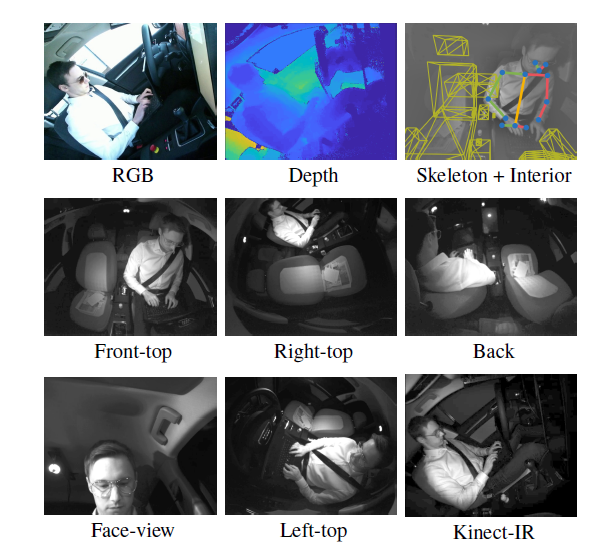
\includegraphics[width=0.8\textwidth]{Images_Thesis/daa_images/Capture_views_thesis.PNG}
\end{center}
\caption[Illustrative images depicting the action of working on a laptop from various views and using different modalities.]{Illustrative images depicting the action of working on a laptop from various views and using different modalities. Source:~\citep{martin2019drive_and_act_2019_iccv}.}
\label{fig:driveandact_views_modalities}
\end{figure}

\subsection{Challenges of the Drive and Act Dataset}
\label{section:Disadvantages of Drive and Act Dataset}
The distribution of all 83 driver actions provided by the \gls{daa} video dataset is depicted in figure~\ref{fig:driveandact_activities}. Each activity is captured for a duration of 3 seconds in one video sample~\citep{martin2019drive_and_act_2019_iccv}. In the figure~\ref{fig:driveandact_activities}, the y-axis depicts the frequency of each activity, while the x-axis represents the 83 activities. It is evident from the figure ~\ref{fig:driveandact_activities} that an important obstacle in the \gls{daa} video dataset is the unequal distribution of classes among all 83 activities including the 34 fine-grained activities~\citep{martin2019drive_and_act_2019_iccv}. This disparity is a substantial obstacle for creating models that can effectively identify rare but potentially vital driving behaviors.~It is crucial to address this issue in order to develop strong models that can accurately detect a variety of actions, including some that are less frequent but may have greater potential for harm. 

\begin{figure}[h]
\begin{center}
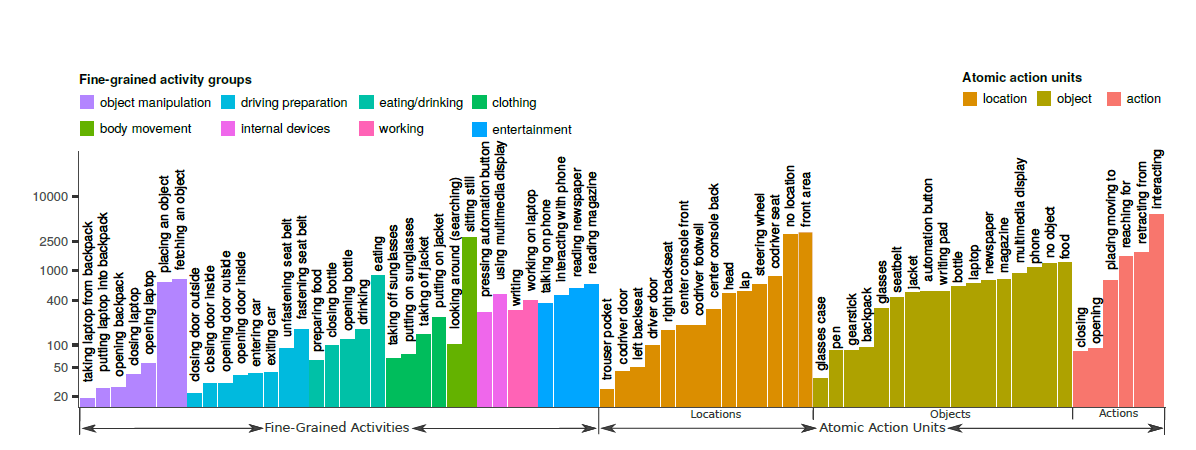
\includegraphics[width=0.8\textwidth]{Images_Thesis/daa_images/Capture_Activities_thesis.PNG}
\end{center}
\caption[Distribution of activities offered by Drive and Act video dataset.]{Distribution of Activities in the Drive and Act Video Dataset. The x-axis represents fine-grained activities, followed by atomic action units, while the y-axis shows the number of video samples, ranging from 0 to 10,000. Source:~\citep{martin2019drive_and_act_2019_iccv}.}
\label{fig:driveandact_activities}
\end{figure}

\subsection{Comparing Drive and Act to Other Datasets}
The \gls{daa} dataset~\citep{martin2019drive_and_act_2019_iccv} is distinguished from current datasets such as NTU~\citep{DBLP:journals/corr/NTUShahroudyLNW16}, HEH~\citep{HEHOhnBar2014HandGR}, AUC~\citep{DBLP:journals/corr/AUCDDAbouelnagaEM17} and Kinetics~\citep{DBLP:journals/corr/KineticsCarreiraZ17} by its large size, wide range of activities recorded, and inclusion of both manual and automated driving situations for Action Recognition. 
For example, the AUC dataset~\citep{DBLP:journals/corr/AUCDDAbouelnagaEM17} contains only 17,000 images, and the NTU dataset~\citep{DBLP:journals/corr/NTUShahroudyLNW16} contains 4 million images, both of which are significantly smaller than the over 9.6 million images provided by the DAA dataset. The Kinetics~\citep{DBLP:journals/corr/KineticsCarreiraZ17} contains more than 76 million images and is exception in terms of size, however it only offers one camera view compared to 6 camera views in \gls{daa} dataset. This comprehensive approach distinguishes it as a significant resource for the research community and highlights its potential to promote breakthroughs in driver behavior identification systems. However, there is an urgent requirement for creative solutions to address the issues of class imbalance and to efficiently utilize the dataset's multi-modal and multi-view data. This dataset provides unparalleled opportunity for researchers in a broad range of domains, particularly in tackling the issue of imbalanced datasets. It enables the \gls{daa} dataset to be bench-marked against the most recent models in a variety of domains, including multi-class and binary classification, view and modality generalization, and the creation of hybrid approaches that use multi-modal technology. These cutting-edge technologies are essential for driver distraction detection, behavior tracking, and the creation of intelligent perceptual user interfaces. By leveraging cutting-edge technology across multiple modalities, this dataset sets the path for major developments in understanding and increasing driver safety and interaction.

In this thesis, we focus on two data modalities from the \gls{daa} dataset: Color and Infrared. An illustration of these modalities, as seen in the action of working on a laptop, is shown in Figure~\ref{fig:driveandact_views_modalities}. The \gls{daa} dataset, derived from video captured with Kinect and NIR cameras, serves as the source of video data for this research. The transformation of this video data into image data is accomplished by extracting frames, a process guided by the dataset's annotation files across all splits. This thesis explores the challenges posed by the significant class imbalance found within these image datasets, a phenomenon that is often extrinsic~\citet{5128907Haibo_Imbalance}. For example, categorizing actions from the \gls{daa} dataset into distracted versus non-distracted classes introduces an inherent imbalance due to varying sample sizes across the 34 fine-grained classes present in the mid-level hierarchical labeling of the \gls{daa} dataset, and can be seen in the figure~\ref{fig:driveandact_activities}. Chapter~\ref{chapter:proposed_methods} provides a detailed analysis of the image datasets and tackle the difficulties caused by imbalanced datasets by proposing and explaining the `Clustered Feature Weighting' algorithm.

\subsection{Key Challenges Posed by Imbalanced Datasets}
Researchers such as~\citep{5128907Haibo_Imbalance, Survey_DL_Taghi_article}, summarised the key challenges posed by imbalanced datasets as follows:
\begin{itemize}
    \item \textbf{Model Bias:} Models trained on imbalanced data typically exhibit a bias towards the majority class, leading to insufficient representation and prediction of minority classes~\citep{imbalance_kC_rawat2022review, 5128907Haibo_Imbalance}.
    \item \textbf{Poor Generalization:} Models may generalize poorly on new, unseen data, especially for under-represented classes~\citep{5128907Haibo_Imbalance, Survey_DL_Taghi_article}.
    \item \textbf{Evaluation Challenges:} Conventional accuracy measurements can be false as they may primarily indicate the frequency of the dominant category rather than the actual prediction capacity of the model in various situations~\citep{5128907Haibo_Imbalance, Survey_DL_Taghi_article}.
\end{itemize}

\section{Existing Solutions to Imbalanced Datasets}
In machine learning, deep learning, and computer vision, learning from datasets that are imbalanced has become a major problem that makes it hard to get high-performance algorithmic results. An imbalanced dataset is characterized by an unequal distribution of classes, a topic that has been extensively explored in the existing literature~\citep{Fernndez2018LearningFI}, ~\citep{5128907Haibo_Imbalance}. This imbalance can develop either organically, as a result of the inherent differences in the frequency of data occurrence, as shown in medical diagnostics, or extrinsically, due to external factors such as the methods used to collect data~\citep{articleSurveyImData},~\citep{5128907Haibo_Imbalance}). According to~\citet{articleKrawczyk}, it is possible to achieve appropriate outcomes regardless of class imbalance, as long as both classes for example in binary classification are sufficiently represented and come from separate distributions~\citep{articleSurveyImData}.

Within the field of image classification, extensive study has been conducted on the issue of imbalance in both binary and multi-class frameworks, resulting in the development of numerous strategies for reducing imbalance problems~\citep{5128907Haibo_Imbalance,H_13_chawla2002smote,H_44_han2005borderline,H_45_he2008adasyn}. However, the usefulness of these strategies varies depending on the application instance, with each approach having its own set of advantages and drawbacks. Traditionally, research has concentrated mostly on machine learning models~\citep{H_75_akbani2004applying, H_77_vilarino2005experiments, H_78_kang2006eus, H_81_tang2006granular}. Nonetheless, current advances in the field of computer vision, natural language processing~\citep{NLP_chen2021multi} and deep learning need a move toward investigating how deep learning models can tackle data imbalance problems or how efficient they are when exposed to imbalanced data~\citep{articleSurveyImData}. According to~\citet{articleJapkowicz2systematicstudy}, the severity of the imbalance problem depends on the degree of class imbalance, the complexity of data representation, the volume of training data, and the classification technique used~\citep{AjayDBLP:journals/corr/abs-2108-00071}.
The Imbalance Ratio (ImR) is a metric that measures the degree of class imbalance. It is calculated as the ratio of the number of samples in the majority class to the number of samples in the minority class~\citep{Fernndez2018LearningFI}. With respect to binary image classification, the terms `majority class' or `negative class' refer to the class with the most samples, whereas `minority class' or `positive class' implies the class with the fewest examples~\citep{AjayDBLP:journals/corr/abs-2108-00071}. The same terminology can be transferred to the domain of multi-class image classification problems.

In order to mitigate the consequences of imbalance, a number of measures are outlined in~\citep{Survey_DL_Taghi_article}. The following are the main solutions:
\begin{itemize}
    \item \textbf{Resampling Techniques:} The dataset can be balanced by oversampling minority classes or undersampling majority classes~\citep{5128907Haibo_Imbalance,Survey_DL_Taghi_article}.
    \item \textbf{Evaluation Metrics:} Adoption of metrics such as the balanced accuracy score, precision, recall, F-1 score, and the area under the Receiver Operating Curve (AUC-ROC) provide a more accurate measure of model performance in the context of imbalanced data~\citep{Survey_DL_Taghi_article, 18_wang2016training}.
    \item \textbf{Class Weight Adjustments:} During model training, adjusting class weights compensates for imbalances by assigning greater importance to minority classes within the loss function~\citep{Survey_DL_Taghi_article}.
\end{itemize}


\subsection{Learning from Imbalanced datasets}
The seminal work ``Learning from Imbalanced Data" by~\citet{5128907Haibo_Imbalance} not only offers a thorough examination of the challenges posed by datasets characterized by under-representation and substantial class imbalances, but also provides practical recommendations for addressing these issues. This study elucidates the difficulties conventional machine learning techniques, which are typically designed for balanced class distributions, encounter in the face of pronounced class disparities. It underscores the inadequacy of traditional metrics, such as overall accuracy~\citep{metric_accuracy_grandini2020metrics} or error rate, in accurately evaluating the performance of algorithms in imbalanced learning scenarios.~\citet{5128907Haibo_Imbalance} advocate for the adoption of more sophisticated evaluation methods, such as receiver operating characteristics (ROC) curves~\citep{ROC_intro_fawcett2006introduction}, precision-recall curves~\citep{precision_recall_giglioni2021use}, and cost curves~\citep{precision_recall_giglioni2021use}, which provide a more detailed insight into performance dynamics. Additionally, the paper highlights the challenges posed by relative imbalances—common in real-world settings—and the significant learning obstacles introduced by the scarcity of representative data for rare instances. Importantly, the authors acknowledge the complexity of datasets and relative imbalances as key contributors to the degradation of classification performance, further exacerbated by factors such as within-class imbalances and small disjuncts~\citep{5128907Haibo_Imbalance}. The authors have presented a comprehensive categorization of solutions available for addressing the issue of learning from imbalanced datasets, as depicted in figure~\ref{fig:imb-learn-tech}. They have also provided detailed explanations for each category and method. Additionally, they have offered criticisms of commonly used solutions, such as sampling methods designed to balance datasets. These critiques address the limitations of undersampling and oversampling, such as the possibility of losing important information and the potential for overfitting.~\citet{5128907Haibo_Imbalance} express significant criticism towards the~\gls{smote}~\citep{H_13_chawla2002smote} method, highlighting its vulnerability to overgeneralization and variance issues. Specifically, the~\gls{smote} algorithm's tendency to generate synthetic data without careful consideration, which might unintentionally blur class boundaries or in other words obscure the distinction between different classes as originally highlighted by~\citep{43_wang2004imbalanced}. The blurring of class boundaries poses challenges for models in differentiating between classes due to the potential resemblance or encroachment of synthetic data points onto the data space of the majority class, or the inaccurate representation of the minority class. This could potentially diminish the efficacy of the model, as it may encounter difficulties in appropriately categorizing novel instances that lie in close proximity to these indistinct boundaries~\citep{43_wang2004imbalanced}.


\tikzset{%
    ,parent/.style={align=left,text width=3cm,rounded corners=1pt}
    ,child/.style={align=left,text width=6.7cm,rounded corners=1pt}
    }
   
\begin{figure}[htbp]
    \centering
    \small
    \begin{forest}
        for tree={%
            ,scale=.55
            ,grow'=east
            ,forked edges
            ,draw
            ,rounded corners
            ,node options={align=left}
            ,text width=4cm
            ,anchor=west
            }
        [Imbalanced Learning\\Techniques~\citep{5128907Haibo_Imbalance}, fill=gray!25, parent
            [Sampling Techniques for Imbalanced Learning, tier=align here, 
            for tree={fill=brown!25, child}
                [Random Oversampling and Undersampling]
                [Informed Undersampling
                    [EasyEnsemble $\&$ BalanceCascade\citep{H_40_liu2008exploratory}]
                    [KNN based:(NearMiss-1)~(NearMiss-2)~(NearMiss-3)~(Most Distant)~\citep{H_41_mani2003knn}]
                    [One-sided selection (OSS)~\citep{H_42_kubat1997addressing}]
                ]
                [Synthetic Sampling with Data Generation
                    [\gls{smote}~\citep{H_13_chawla2002smote}]
                ]
                [Adaptive Synthetic Sampling
                    [Borderline-\gls{smote}~\citep{H_44_han2005borderline}]
                    [Adaptive Synthetic Sampling~\citep{H_45_he2008adasyn}]
                ]
                [Sampling with Data Cleaning
                    [Tomek links~\citep{H_46_tomek1976two_4309452}]
                    [OSS method~\citep{H_42_kubat1997addressing}]
                    [Condensed nearest neighbor rule and Tomek Links~\citep{H_22_batista2004study}]
                    [Neighborhood Cleaning Rule~\citep{H_36_laurikkala2001improving}]
                    [\gls{smote} $+$ ENN and \gls{smote} $+$ Tomek~\citep{H_22_batista2004study}]
                ]
                [Cluster-Based Sampling
                    [Cluster-based oversampling~\citep{H_27_jo2004class}]
                ]
                [Integration of Sampling and Boosting
                    [\gls{smote}-Boost~\citep{H_47_chawla2003smoteboost}]
                    [Data-Boost-IM~\citep{H_14_guo2004learning}]
                    [JOUS-Boost~\citep{H_38_mease2007boosted}]
                ]
            ]
            [Cost-Sensitive Approaches, 
            for tree={fill=red!25,child}
                [Cost-Sensitive Learning Framework
                    [Translation theorem~\citep{H_55_zadrozny2003cost}] 
                    [Metacost framework~\citep{H_54_domingos1999metacost}]
                ]
                [Cost-Sensitive Dataspace Weighting with Adaptive Boosting
                    [(AdaC1)~(AdaC2)~(AdaC3)~\citep{H_58_sun2007cost}] 
                    [AdaCost~\citep{H_59_fan1999adacost}]
                ]
                [Cost-Sensitive Decision Trees and Neural Networks]
            ]
            [Kernel-Based Methods, tier=align here, 
            for tree={fill=blue!25, child}
                [Kernel-Based Learning Framework
                    [~\gls{svm}~\citep{H_23_japkowicz2002class}]
                ]
                [Kernel Methods with Sampling
                    [\gls{smote} with Different Costs~\citep{H_75_akbani2004applying}] 
                    [Ensembles of over/undersampled~\gls{svm}~\citep{H_77_vilarino2005experiments}~\citep{H_78_kang2006eus}~\citep{H_79_liu2006boosting}~\citep{H_80_wang2008boosting}] 
                    [Granular \gls{svm}—Repetitive Undersampling~\citep{H_81_tang2006granular}]
                ]
                [Kernel Modification Methods
                    [Kernel classifier construction~\citep{H_85_hong2007kernel}] 
                    [(Boundary movement)~(Biased penalties)~(Class-boundary alignment)~\citep{H_76_wu2003class}] 
                    [Kernel-boundary alignment~\citep{H_86_wu2004aligning}~\citep{H_87_wu2005kba}] 
                    [k-category Proximal \gls{svm} with Newton refinement~\citep{H_91_fung2001proximal}] 
                    [Support cluster machines~\citep{H_92_yuan2006learning}] 
                    [Kernel neural gas for imbalanced clustering~\citep{H_93_qin2004kernel}] 
                    [(P2PKNNC algorithm)~(P2P communication paradigm)~\citep{H_94_yu2007novel}]
                ]
            ]
            [Active Learning Methods, 
            for tree={fill=green!25, child}
                [Simple active learning heuristic~\citep{H_103_doucette2008gp}]
            ]
            [Supplementary Approaches, tier=align here, 
            for tree={fill=orange!25, child}
                [One-class \gls{svm}~\citep{H_74_raskutti2004extreme}] 
                [Autoassociator method~\citep{H_109_japkowicz2001supervised}~\citep{H_110_manevitz2007one}~\citep{H_111_japkowicz2000learning}~\citep{H_112_japkowicz1995novelty}] 
                [Ensemble knowledge for imbalance sample sets (eKISS)~\citep{H_12_tan2003multi}]
            ]
        ]
    \end{forest}
    \caption[Classification of Imbalanced Learning Techniques]{A flow chart showing the classification of Imbalanced Learning Techniques proposed by~\citet{5128907Haibo_Imbalance}.}
    \label{fig:imb-learn-tech} % Label for cross-referencing
\end{figure} 

Additionally,~\citet{Data_algo_hybrid_krawczyk2016learning} categorize the strategies for addressing imbalanced datasets into three principal techniques. Initially, they examine data-level approaches, which involve adjustments to the sampling process either to balance the class distribution or to eliminate problematic samples. The second category encompasses algorithm-level strategies, which modify the core learning algorithms to better manage data with skewed distributions, thereby reducing the bias towards majority class instances~\citep{Data_algo_hybrid_krawczyk2016learning, Fernndez2018LearningFI}. Subsequently,\citet{Data_algo_hybrid_krawczyk2016learning} provide hybrid methods that combine the benefits of both data-level and algorithm-level approaches~\citep{Navo_Im_chakrabarty2020navo}.

\citet{Fernndez2018LearningFI} explored the challenges associated with learning from imbalanced datasets thoroughly in \textit{Learning from Imbalanced Data Sets}~\citep{Fernndez2018LearningFI}. Similarly, \citet{Survey_DL_Taghi_article} provide a detailed review of methods to tackle class imbalance in machine learning, with an emphasis on deep learning techniques. \citet{Survey_DL_Taghi_article} categorizes the various techniques, defines appropriate assessment criteria for imbalanced datasets, and underscores the significance of both supervised and unsupervised learning approaches, including those that incorporate transfer learning. \citet{Survey_DL_Taghi_article} notes that traditional metrics like accuracy can misleadingly reflect performance in imbalanced contexts due to their susceptibility to the prevalence of the majority class~\citep{Fernndez2018LearningFI, Survey_DL_Taghi_article}. Instead, Balanced Accuracy (BA)~\citep{bal_acc_paper_brodersen2010balanced} is recommended as it accounts for both the True Positive Rate (TPR) and the True Negative Rate (TNR), offering a comprehensive measure of model efficacy across both majority and minority classes and mitigating the inherent bias of simpler metrics~\citep{18_wang2016training}. \citet{Survey_DL_Taghi_article} identifies a gap in the exploration of deep learning strategies for managing class imbalance, with most current methods, particularly those involving sampling or algorithmic modifications, falling within the domain of supervised learning due to their reliance on labeled data for adjusting class distributions or refining learning algorithms based on class-specific insights~\citep{Survey_DL_Taghi_article}. The discourse also touches on innovative deep learning techniques such as dynamic sampling, two-phase learning, and enhancements involving novel loss functions and cost-sensitive learning~\citep{Survey_DL_Taghi_article}. Additionally, the integration of transfer learning with deep learning strategies to enhance model performance on imbalanced datasets is discussed. Despite the prevalence of supervised methods, the field of unsupervised learning in relation to class imbalance remains under-explored and represents a promising area for future research.

\subsection{Transfer Learning and Clustering-Based Techniques}
Transfer learning is an advantageous approach in deep learning that can address the problem of class imbalance. By initially training on diverse and wide datasets and then fine-tuning the model on the unbalanced dataset, it is possible to strengthen the model's capacity to generalize its knowledge to new scenarios and enhance its overall performance~\citep{Survey_DL_Taghi_article}. This approach is especially beneficial for classes that have a restricted number of examples, as conventional learning methods may lead to below-average model performance~\citep{Survey_DL_Taghi_article}. The review paper discusses various methods, such as category centers (CC) proposed by~\citet{91_zhang2018image}, Large Margin Local Embedding (LMLE) introduced by~\citet{22_huang2016learning}, and Deep Over Sampling (DOS) developed by~\citet{117_ando2017deep}. These methods utilize hybrid approaches that combine transfer learning, deep feature representations, and k-nearest neighbors to tackle imbalanced datasets~\citep{Survey_DL_Taghi_article}.

Clustering-based methods have become a sophisticated approach to tackle class imbalance by focusing on grouping instances into clusters before applying subsampling methods. This strategy aims to preserve the integrity of information while simultaneously providing a more equitable distribution among different classes~\citep{densitybased_IM_munguia2023density}. More precisely, algorithms such as K-means~\citep{kmeans_kaufman2009finding} and \gls{clara}~\citep{kmeans_kaufman2009finding} aid in the creation of clusters within classes by choosing instances that are both representative and diverse. A significant progress in this field is the utilization of density-based clustering methods, specifically \gls{dbscan}~\citep{DBSCAN_algo_ester1996density} and \gls{hdbscan}~\citep{HDBSCAN_algo_campello2013density}. These algorithms excel at handling datasets with varying sizes, shapes, and densities by detecting regions with high population density. This allows for reducing the size of the majority class without significant loss of information~\citep{densitybased_IM_munguia2023density}.


\citet{densitybased_IM_munguia2023density} makes a comprehensive contribution by presenting a new density-based undersampling technique that exploits the capabilities of \gls{dbscan} and \gls{hdbscan}, in addition to an improved \gls{scut}~\citep{SCUT_agrawal2015scut} algorithm. This approach, when used with imbalanced and multi-class hyperspectral remote sensing images, employs geometric mean values and Friedman's test~\citep{Friedman_Test_7c3c84e5-7230-3033-8b6c-ec430fb73d61} to thoroughly assess its effectiveness. The results emphasize the effectiveness of density-based clustering methods in addressing the difficulties posed by severe class imbalances, representing a notable shift from conventional strategies~\citep{densitybased_IM_munguia2023density}.

~\citet{densitybased_IM_munguia2023density} introduces methodological advancements that suggest a more precise equilibrium between undersampling and oversampling, depending on the average size of each class sample. This strategy effectively combines density-based clustering with the \gls{scut} method to dynamically modify class sizes. It utilizes \gls{dbscan}~\citep{DBSCAN_algo_ester1996density} or \gls{hdbscan}~\citep{HDBSCAN_algo_campello2013density} for classes that are above the average and employs \gls{smote}~\citep{H_13_chawla2002smote} for classes that are below the average. This strategy seeks to achieve both a more equitable representation of classes and improved classifier performance by utilizing geometric mean values as a measure of success. The suggested method effectively addresses the issue of class imbalance by deliberately removing instances from the majority class using density-based clustering and increasing the representation of the minority class through \gls{smote}. The empirical validation of this method, which shows significant improvements in the accuracy of classifying highly unbalanced datasets, highlights the potential of combining density-based clustering with sampling approaches as an effective solution to the challenges caused by class imbalance.

The research by~\citet{densitybased_IM_munguia2023density} contends that conventional oversampling techniques such as \gls{smote} and its variations aim to achieve balance in the dataset, but they may not adequately address the nuances of class imbalance. On the other hand, clustering methods, especially those that rely on density, provide a strong and reliable alternative.

\paragraph{Research Gap:}~The emergence of~\gls{vit} models has had a tremendous impact on the field of computer vision. Despite this advancement, the use of these models to address the common issue of dataset imbalance has not been widely examined. This oversight signifies a crucial research gap, neglecting the potential of \gls{vit} models to serve as general-purpose tools for extracting intricate image features. Vision Transformers are distinguished by their ability to assimilate complex visual representations, which provides access to a rich feature space for developing novel techniques to handle the imbalanced learning challenge. This feature space, strengthened by training on large and diverse image datasets, has a wide range of visual properties. Such a collection of information is useful in finding both tiny differences and similarities between images, presenting a viable solution to the imbalance problem. It offers a thorough understanding and representation of minority classes, which are typically excluded and ignored by standard models. The comprehensive representation offered by \gls{vit} models opens up opportunities for the advancement of sampling strategies, augmentation techniques, and customized loss functions that are particularly crafted to address the distinct difficulties presented by unbalanced datasets. By innovating techniques that exploit the feature space of Vision Transformers~\citep{Vit_Paper_Dosovitskiy2020AnII}, there lies the potential to inaugurate a new phase of progress in deep learning. This advancement is particularly crucial in achieving equitable and consistent model performance across all class categories within imbalanced datasets.


Within the context of this thesis, Chapter~\ref{chapter:proposed_methods} focuses on introducing and explaining such a novel sampling technique called ``ClusteredFeatureWeighting" that combines the effective use of feature space of \gls{vit} using Transfer Learning, Density-Based Clustering, and Weighted Random Sampling. This novel approach is specifically tailored to rectify the imbalance dataset problem inherent in the drive and act dataset~\citep{martin2019drive_and_act_2019_iccv}. Subsequent chapters, particularly Chapters~\ref{chapter:background} and~\ref{chapter:proposed_methods}, provide a comprehensive explanation of the working principles and experimental methodologies. Chapter~\ref{chapter:Experiments and Results} presents the results after each experiment by employing the methodology explained in the chapter~\ref{chapter:proposed_methods}.




%%%%%%%%%%%%%%%%%%%%%%%% Chapter 3: Background %%%%%%%%%%%%%%%%%%%%
% Equation (1): Initial Embeddings
% - z_0: The initial sequence of embeddings that will be inputted into the Transformer encoder.
% - x_class: A learnable embedding that represents the classification token, similar to BERT's [class] token.
% - x_p^i: The flattened vector of the i-th image patch.
% - E: The trainable linear projection matrix that maps the flattened image patches into D dimensions.
% - N: The total number of patches into which the image is divided.
% - E_pos: The position embeddings added to the patch embeddings to give the model information about the order of the patches.
% - +: Denotes concatenation of the classification embedding and the patch embeddings, followed by element-wise addition of position embeddings.

% Equation (2): Multiheaded Self-Attention (MSA) and Residual Connection
% - z'_l: The output of the multiheaded self-attention (MSA) block for layer l after adding the residual connection.
% - MSA: Multiheaded self-attention function that allows the model to focus on different parts of the sequence.
% - LN: Layernorm function that normalizes the input across features.
% - z_{l-1}: The output of the previous layer or the initial embeddings for l = 1.

% Equation (3): MLP Block and Residual Connection
% - z_l: The output of the MLP block for layer l after adding the residual connection.
% - MLP: Multilayer perceptron function, which is a feedforward neural network that can model complex functions.
% - LN: Layernorm function applied again to normalize the inputs for the MLP block.
% - z'_l: The output from the self-attention block which serves as an input to the MLP block.

% Equation (4): Final Output Representation
% - y: The final image representation used for classification.
% - LN: The layernorm function applied to the output of the last layer.
% - z_L^0: The output of the Transformer encoder corresponding to the classification token.
% - L: The total number of layers in the Transformer encoder
%%%%%%%%%%%%%%%%%%%%%%%%%%%%%%%%%%%%%%%%%%%%%%%%%%%%%%%%%%%%%%%%%%%
\chapter{Background}
\label{chapter:background}
We looked at the study on driver distraction detection and dataset imbalance in the last chapter. Following the research gaps identified in the previous section and the recommended research alternatives, this chapter will look at the background knowledge and working principles of the algorithms and models employed in this thesis to address the research problems. It covers the working principle of the HDBSCAN clustering algorithm~\citep{HDBSCAN_algo_campello2013density} and vision transformer~\cite{Vit_Paper_Dosovitskiy2020AnII}. Also discussed are the \gls{din}~\citep{dino_caron2021emerging} framework and it's improved version \gls{dino}~\citep{dinov2_oquab2023dinov2} for training vision transformer models.

\section{HDBSCAN Clustering Algorithm}
Clusters can be represented as dense regions in the data space, divided by sparse areas. Density-based clustering algorithms use this strategy to identify non-spherical groupings~\citep{density_based_clustering_book_han2011data}. Density-based clustering detects clusters in data by separating regions of high and low point density ~\citep{density_based_clustering_book_han2011data}. DBSCAN~\citep{DBSCAN_algo_ester1996density} is a type of density based clustering algorithm which groups points that are closely packed together, marking points that are in low-density regions as noise. This method is particularly effective for discovering clusters of arbitrary shapes and sizes in datasets with noise~\citep{hdbscanComparingPython}. While DBSCAN~\citep{DBSCAN_algo_ester1996density} is powerful, it has limitations. It requires two parameters: \textit{eps} (maximum distance between neighbors) and \textit{min\_samples} (minimum number of points to form a dense region)~\citep{DBSCAN_algo_ester1996density, hdbscanComparingPython}. Selecting suitable values for these variables might prove problematic, especially for datasets with varying density~\citep{hdbscanComparingPython}. Moreover, DBSCAN~\citep{DBSCAN_algo_ester1996density} does not inherently provide a way to explore the hierarchical structure of clusters~\citep{hdbscanComparingPython}.

HDBSCAN (Hierarchical Density-Based Spatial Clustering of Applications with Noise)~\citep{HDBSCAN_algo_campello2013density} extends DBSCAN~\citep{DBSCAN_algo_ester1996density} by addressing these limitations. It combines density-based clustering with hierarchical clustering, allowing it to handle data with varying density more effectively and revealing a hierarchy of clusters~\citep{hdbscanComparingPython}.

\newpage

\paragraph{Working of HDBSCAN algorithm:} Based on the~\citep{HDBSCAN_algo_campello2013density, HDBSCAN_2015_campello2015hierarchical} papers, the working of HDBSCAN algorithm can be divided into following steps:

\begin{enumerate}
    \item \textbf{Transforming the Space}:
    \begin{itemize}
        \item HDBSCAN begins by computing the core distance for each point, which represents the distance to its $k$-th nearest neighbor (where $k$ is defined by the \textit{min\_samples} parameter).
        \item It then calculates the mutual reachability distance between pairs of points. This distance accounts for the core distance of the points, ensuring clusters can be identified in regions with varying density.
    \end{itemize}
    
    \item \textbf{Building the Minimum Spanning Tree (MST)}:
    \begin{itemize}
        \item Using the mutual reachability distances, HDBSCAN constructs a minimum spanning tree (MST). This tree connects all points in the dataset with the shortest possible total distance, ensuring every point is reachable from any other point~\citep{hdbscanComparingPython}.
    \end{itemize}
    
    \item \textbf{Condensing the Tree}:
    \begin{itemize}
        \item The MST is condensed into a hierarchy of connected components by progressively removing the edges with the longest mutual reachability distances. This process reveals a tree structure, or dendrogram, that represents clusters at different density levels~\citep{hdbscanComparingPython}.
    \end{itemize}
    
    \item \textbf{Extracting Stable Clusters}:
    \begin{itemize}
        \item From the dendrogram, HDBSCAN uses the Excess of Mass (EOM) method to extract clusters. EOM identifies the most stable clusters by measuring their persistence across different density levels. Stable clusters are those that remain consistent over a range of scales, indicating they are meaningful groupings of data points~\citep{hdbscanComparingPython}.
    \end{itemize}
    
    \item \textbf{Outlier Detection}:
    \begin{itemize}
        \item Points that do not belong to any stable cluster are labeled as noise. These points are in low-density regions and do not fulfill the requirements to be considered as part of a cluster~\citep{HDBSCAN_algo_campello2013density, HDBSCAN_2015_campello2015hierarchical}.
    \end{itemize}
\end{enumerate}

\paragraph{Key Parameters of HDBSCAN:}

\begin{itemize}
    \item \textbf{Minimum Cluster Size (e.g., 25)}: Sets the smallest allowable size for a cluster. Clusters smaller than this are considered noise.
    \item \textbf{min\_samples (e.g., 1)}: Specifies the minimum number of points required within a neighborhood for a point to be classified as a core point, hence affecting the computations of local density~\citep{HDBSCAN_algo_campello2013density, HDBSCAN_2015_campello2015hierarchical, hdbscanComparingPython}.
    \item \textbf{cluster\_selection\_epsilon (0.0)}: Controls the sensitivity for cluster formation. A value of 0.0 applies the strictest criteria.
    \item \textbf{metric (`euclidean')}: Specifies the distance metric, with `euclidean' being the default for calculating distances between points~\citep{hdbscanComparingPython}.
    \item \textbf{cluster\_selection\_method (`eom')}: Determines how clusters are selected from the hierarchical tree, with `eom' favoring stable, persistent clusters.
\end{itemize}

HDBSCAN~\citep{HDBSCAN_algo_campello2013density} improves upon traditional density-based clustering by combining it with hierarchical clustering techniques. It enables the HDBSCAN algorithm to efficiently process datasets with different levels of density, detect clusters of any shape, and identify significant clusters more reliably than techniques such as DBSCAN~\citep{DBSCAN_algo_ester1996density}. Through its use of core distances, mutual reachability distances, and hierarchical extraction methods, HDBSCAN~\citep{HDBSCAN_algo_campello2013density} provides a powerful tool for clustering complex data. While HDBSCAN is relatively less affected by parameter settings compared to other clustering algorithms, it still necessitates the configuration of parameters such as `min\_cluster\_size' and `min\_samples', which can impact the clustering results and is a limitation of this algorithm~\citep{hdbscanComparingPython, HDBSCAN_2015_campello2015hierarchical}.

\section{Vision Transformer}
The \gls{vit}~\citep{Vit_Paper_Dosovitskiy2020AnII}~ has transformed the computer vision domain by demonstrating that \gls{cnn}s~\citep{CNN_o2015introduction} are not necessary for achieving high performance in image classification tasks. ViT applies the Transformer architecture~\citep{Vaswani2017AttentionIA}, originally intended for sequential data in Natural Language Processing (NLP)~\citep{NLP_Book_eisenstein2019introduction}, to process images by considering them as sequences of patches, akin to tokens in text. 

\begin{figure}[h]
\begin{center}
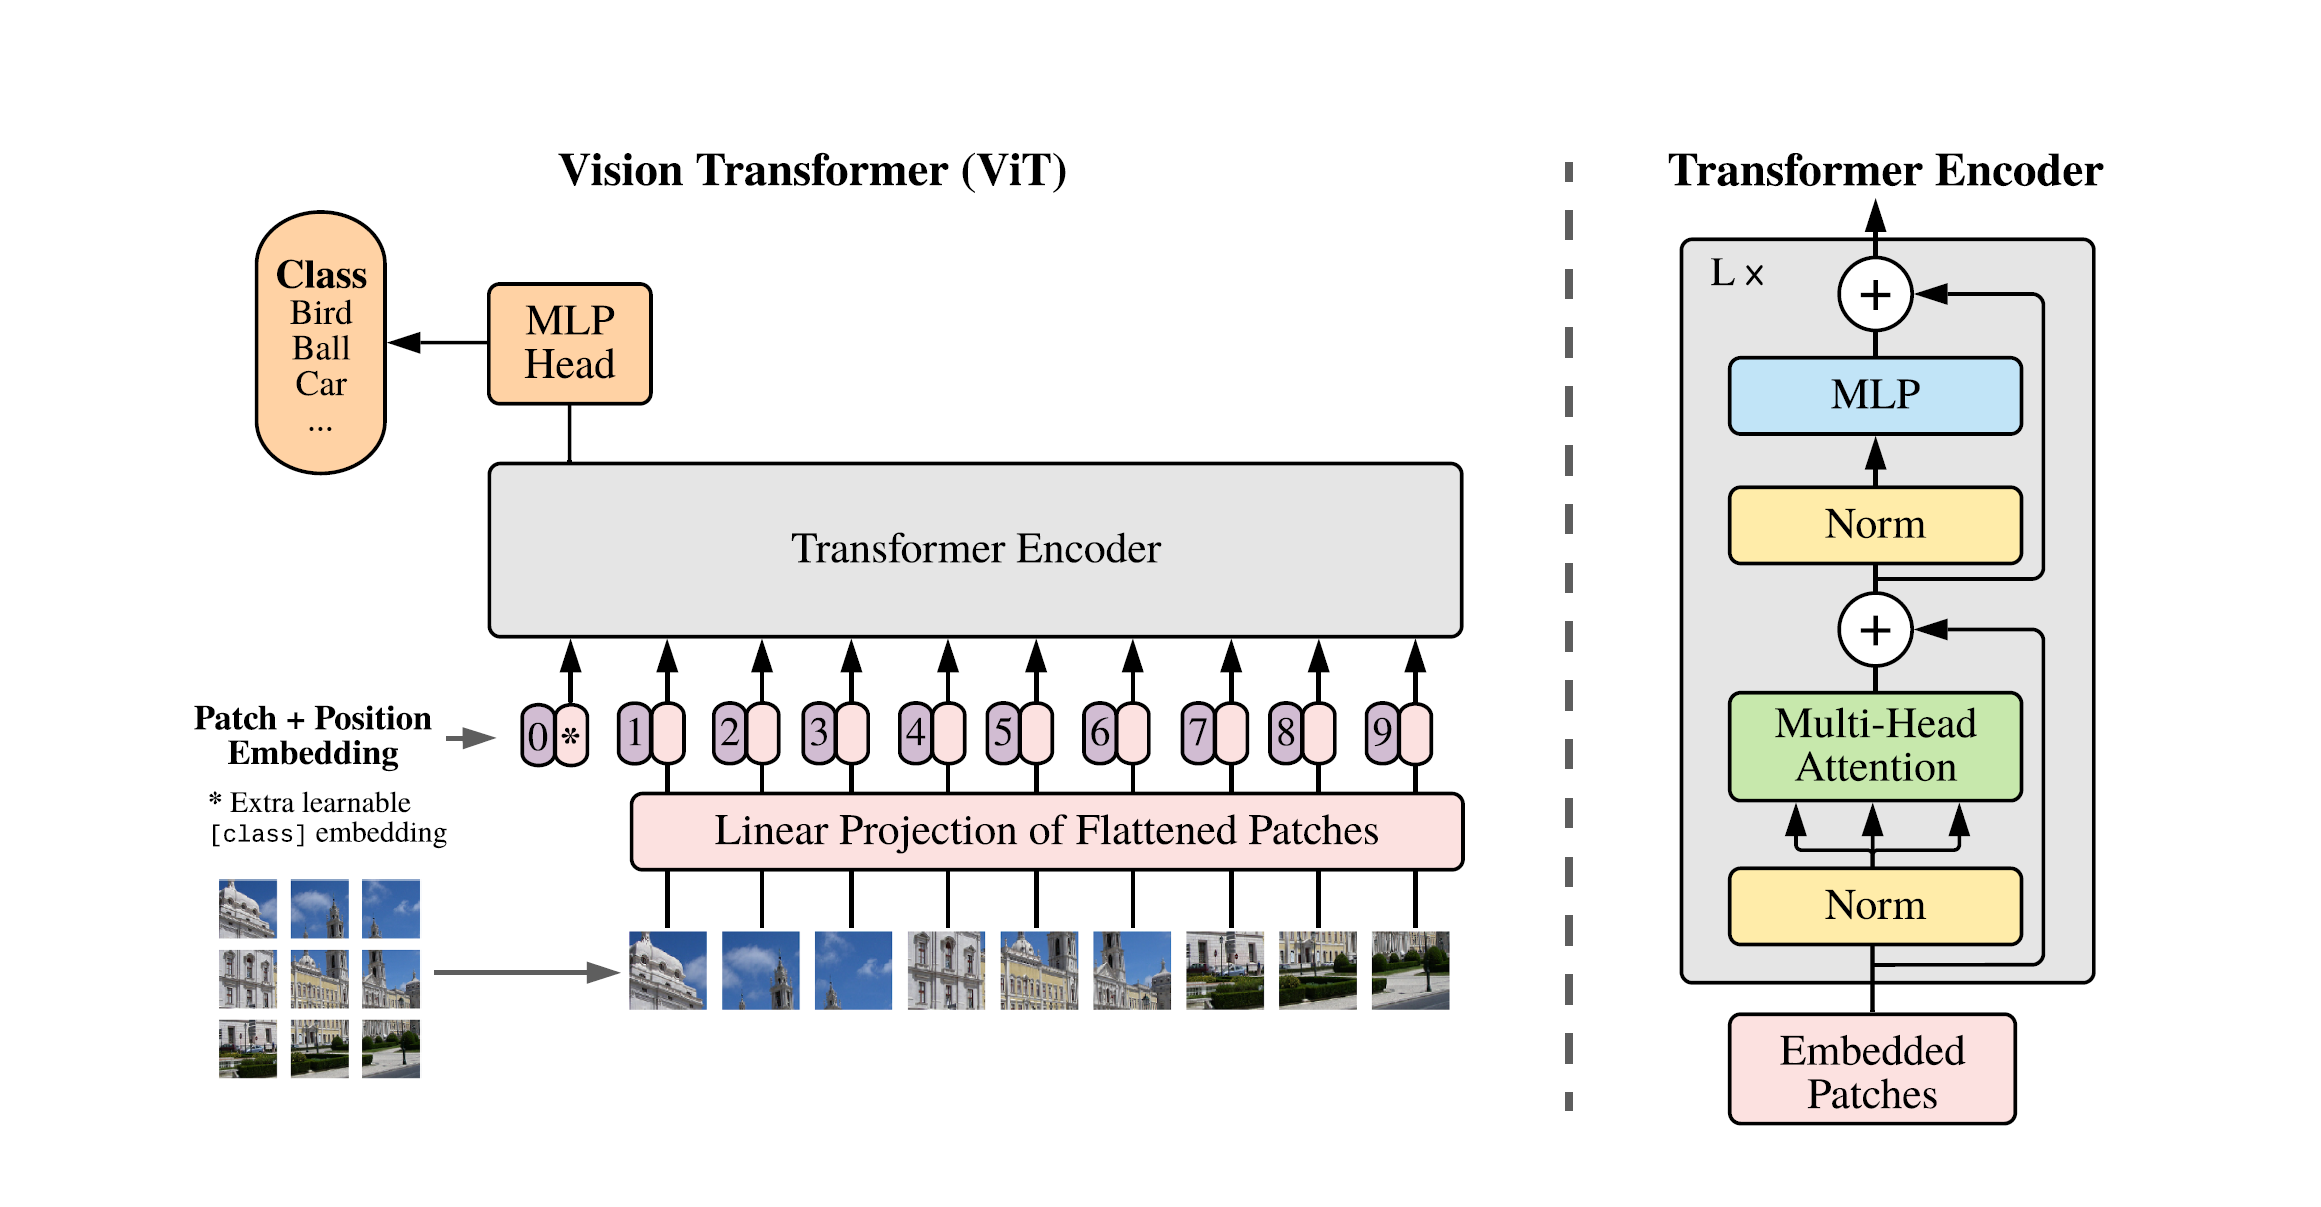
\includegraphics[width=\textwidth]{Vit_arch.png}
\end{center}
\caption[Vision Transformer Architecture]{Vision Transformer Architecture from~\citep{Vit_Paper_Dosovitskiy2020AnII}.}
\label{fig:vit_arch}
\end{figure}

\paragraph{Vision Transformer Architecture:}
The Vision transformer architecture consists of key elements including image patches, patch and positional embedding, learnable class embedding, Transformer Encoder, and MLP Head as shown in figure~\ref{fig:vit_arch}. Image patches are embedded linearly, with position embeddings for spatial information preservation. The transformer encoder is composed of layers that alternate between multi-headed self-attention and MLP blocks. LayerNorm (LN) is applied before each block and residual connections are applied after each block. The MLP blocks have two layers with a GELU non-linearity to maintain local and translational equivariance. The multi-headed self-attention layers record global dependencies across the image~\citep{Vit_Paper_Dosovitskiy2020AnII}.~The MLP Head converts learned features into class output, sometimes it is also referred as the classifier head in classification tasks.

\paragraph{Mathematical Functions and Terminology:}
This paragraph adheres to the notations and conventions established in the Vision Transformer (ViT) paper by~\citet{Vit_Paper_Dosovitskiy2020AnII}. All descriptions and mathematical formulations presented herein are based on those detailed in the original paper.

The process includes transforming image patches into embeddings, adding positional embeddings and a class token, and then passing them through the Transformer encoder, which entails a sequence of essential mathematical operations necessary for understanding the functionality of ViT. The components include linear transformations for patch embedding, softmax normalization in the self-attention mechanism, and the GELU~\citep{GELU_act_fxn_hendrycks2016gaussian} non-linearity in \gls{mlp} blocks.

\citet{Vit_Paper_Dosovitskiy2020AnII} considered an RGB image $\mathbf{x}$ with dimensions $H \times W \times C$, where H represents Height, W represents Width, and C represents the color channel of the image. The image has a resolution of $H \times W$. \citet{Vit_Paper_Dosovitskiy2020AnII} converted this image into a series of 2D image patches by dividing it into $N$ patches with a resolution of $P^2$. 

\citet{Vit_Paper_Dosovitskiy2020AnII} mathematically transformed an image $\mathbf{x}$ into a 2D sequence of image patches $\mathbf{x}_p$, as shown in equation~\ref{equation:3.1}. 

% Centered with equation number
\begin{equation}
\label{equation:3.1}
\mathbf{x} \in \mathbb{R}^{H \times W \times C} \rightarrow \mathbf{x}_p \in \mathbb{R}^{N \times (P^2 \times C)}
\end{equation}
The lowercase letter ``p" represents the patch. The number of patches, N, obtained from this transformation is determined by dividing the resolution of the original image by the resolution of each patch. \citet{Vit_Paper_Dosovitskiy2020AnII} expressed N as the product of H and W divided by P squared as given in equation~\ref{equation:3.2}. 
\begin{equation}
\label{equation:3.2}
N = \frac{H \times W}{P^{2}}
\end{equation}
Afterwards, \citet{Vit_Paper_Dosovitskiy2020AnII} turned the two-dimensional patch sequence into a one-dimensional sequence using linear projections to align with the input requirements of the conventional Transformer encoder~\citep{Vaswani2017AttentionIA}, which only accepts one-dimensional token embeddings. The linearly projected embedding is referred to as Patch embedding and is trainable. 

According to ~\citet{Vit_Paper_Dosovitskiy2020AnII}, the initial patch embeddings and positional encoding of an input image in the Vision Transformer architecture can be defined as:

% \\ for new line and & for concatinationg, \quad for spacing
\begin{equation}
\begin{aligned}
\mathbf{z}_0 & =\left[\mathbf{x}_{\text {class}} ; \mathbf{x}_p^1 \mathbf{E} ; \mathbf{x}_p^2 \mathbf{E} ; \cdots ; \mathbf{x}_p^N \mathbf{E}\right] \\
& \quad +\mathbf{E}_{\text {pos}}, \quad \mathbf{E} \in \mathbb{R}^{\left(P^2 \cdot C\right) \times D}, \quad
\mathbf{E}_{\text {pos}} \in \mathbb{R}^{(N+1) \times D}
\end{aligned}
\label{3.3}
\end{equation}


In equation ~\ref{3.3},~$\mathbf{z}_0$ is the initial embedding matrix input into the Transformer encoder. The image is initially divided into N flattened 2D patches, indicated by $x_{p}^{i}$, where i denotes the count of patches from 1 to N. These patches are then linearly projected into a D-dimensional embedding space using a trainable matrix E~\citep{Vit_Paper_Dosovitskiy2020AnII}. The embedding matrix E is shared by all patches, representing the idea that each patch is equivalent to a `word' in NLP tasks. Position embeddings $\mathbf{E}_{\text {pos }}$ are used to maintain positional information, which is crucial given the Transformer's permutation invariance~\citep{Vit_Paper_Dosovitskiy2020AnII}. A specific class embedding $\mathbf{x}_{\text {class }}$ is prepended to the sequence to serve as a proxy for the overall image representation.


Each Transformer encoder layer comprises a self-attention mechanism~\cite{Vaswani2017AttentionIA}, succeeded by a \gls{mlp}. Mathematically, the self-attention mechanism along with residual connection~\citep{residual_connection_he2016deep} for layer $\ell$ is represented as:

\begin{equation}
\begin{aligned}
\mathbf{z}_{\ell}^{\prime} & =\operatorname{MSA}\left(\operatorname{LN}\left(\mathbf{z}_{\ell-1}\right)\right)+\mathbf{z}_{\ell-1}, & & \ell=1 \ldots L \\
\end{aligned}
\label{3.4}
\end{equation}

In the vision transformer architecture, $\ell$ is a number between 1 and $L$, where $L$ is the maximum number of stacked transformer encoders.~The implementation of the multiheaded self-attention (MSA) function on the layer-normalized embeddings from the preceding layer~ $\mathbf{z}_{\ell-1}$, is illustrated in equation~\ref{3.4}. Subsequently, the result of this combined operation, is added in~$\mathbf{z}_{\ell-1}$~as a residual connection~\citep{residual_connection_he2016deep}, thereby enabling gradient flow~\citep{Vit_Paper_Dosovitskiy2020AnII}. The self-attention mechanism's output~$\mathbf{z}_{\ell}^{\prime}$~ is subsequently passed through a \gls{mlp} in the Transformer encoder block as described in equation~\ref{3.5}:
\begin{equation}
\begin{aligned}
\mathbf{z}_{\ell} & =\operatorname{MLP}\left(\operatorname{LN}\left(\mathbf{z}_{\ell}^{\prime}\right)\right)+\mathbf{z}_{\ell}^{\prime}, & & \ell=1 \ldots L \\
\end{aligned}
\label{3.5}
\end{equation}

The output of the Transformer encoder block is the result of combining the output of the \gls{mlp} with the output of residual connection~\citep{Vit_Paper_Dosovitskiy2020AnII}. The \gls{mlp} comprises two dense layers with a GELU~\citep{GELU_act_fxn_hendrycks2016gaussian} activation function.

Ultimately, equation~\ref{3.6} produces the ultimate output representation of the image, which is subsequently employed for classification purposes.

\begin{equation}
\begin{aligned}
\mathbf{y} & =\operatorname{LN}\left(\mathbf{z}_L^0\right) & &
\end{aligned}
\label{3.6}
\end{equation}

The final image representation, denoted as $y$, is derived by applying layer normalization~\citep{Layer_norm_ba2016layer} to the layer that corresponds to the classification token. This representation $y$ contains the aggregated information from all patches and their interactions as distilled through the various Transformer layers. The Vision Transformer's image classification approach replaces traditional convolutional operations with mechanisms that consider image patches as sequences of data points, akin to words in a sentence. This enables the model to learn contextual relationships throughout the image~\citep{Vit_Paper_Dosovitskiy2020AnII}.

% Attention is a measure of a token's relevance to other tokens, including itself. Key, Value, and Query vectors ar learned by a FFNN. Similarity scores computed from Key, Value and Query. Take softmax of these scores to get attention weights.

\paragraph{Multi-headed Self-Attention Mechanism:}
The primary functionality of ViT relies on self-attention, enabling each patch to attend to every other patch in the image. This mechanism allows the model to prioritize the most pertinent regions of the image for the given task. The multi-headed self-attention~\cite{Vaswani2017AttentionIA} (MHSA) improves the model's ability to understand complex spatial structures and connections by recording several visual components at the same time. The detailed process of self-attention mechanism can be found in paper~\cite{Vaswani2017AttentionIA}, while the mathematical explanation of the Multi-headed Self-Attention mechanism is given in Appendix A of the Vision transformer paper~\cite{Vit_Paper_Dosovitskiy2020AnII}.

\section{Evolution of Self-Supervised Learning in Vision Transformers: From DINO to DINOv2}
DINO stands for ``Self-Distillation with NO labels"~\citep{dino_caron2021emerging}. It is an innovative advancement in self-supervised learning for vision transformers. The \gls{din} framework takes a novel approach to self-supervised learning by merging elements of self-training and knowledge distillation, which have previously been employed to increase feature quality by propagating annotations to unlabeled datasets~\citep{dino_caron2021emerging, _35_kn_distill_hinton2015distilling}. Traditionally, knowledge distillation is teaching a smaller, simpler student network to mimic the behavior of a larger, pre-trained teacher network, therefore compressing knowledge into a more efficient model~\citep{_7_modelcompr_buciluǎ2006model, knowdledge_distill_2017_kim2017transferring, dino_caron2021emerging}. \gls{din} framework innovates by converting this method into what is known as ``self-distillation," in which both the student and the teacher are trained concurrently during the learning phase, with no labeled data. In self-supervised vision transformers, label propagation involves both hard and soft assignments~\citep{_41_pseudo_label_semi_sup_lee2013pseudo,_78_plabel_speech_xu2020iterative,_79_billion_scale_yalniz2019billion, _76_seftraining_xie2020self}, with soft assignments~\citep{_76_seftraining_xie2020self} being particularly matched with knowledge distillation concepts~\citep{_7_modelcompr_buciluǎ2006model,_35_kn_distill_hinton2015distilling}. This strategy has usually concentrated on model compression by training smaller networks to mimic the outputs of bigger ones, as proven by~\citet{_76_seftraining_xie2020self}.

DINO applies these notions to a self-supervised situation in which no true labels are available. Unlike prior techniques, which used a pre-trained, fixed teacher~\citep{_13_big_ssl_chen2020big, _25_SEED_fang2021seed,_63_s2_bnn_shen2021s2,_47_boosting_ssl_KT_noroozi2018boosting}, \gls{din} framework dynamically constructs the teacher during training, making knowledge distillation an inherent component of the learning objective rather than a post-processing step~\citep{dino_caron2021emerging}. This approach is similar to codistillation~\citep{_1_codistillation_anil2018large}, in which both the student and teacher networks share the same architecture; however, in \gls{din}, the teacher network is updated using an exponential moving average~\citep{ema_polyak1992acceleration} of the student's parameters rather than mutual distillation as depicted in the figure~\ref{fig:dino_v1_arch}~\citep{dino_caron2021emerging}.

\begin{figure}[h]
\begin{center}
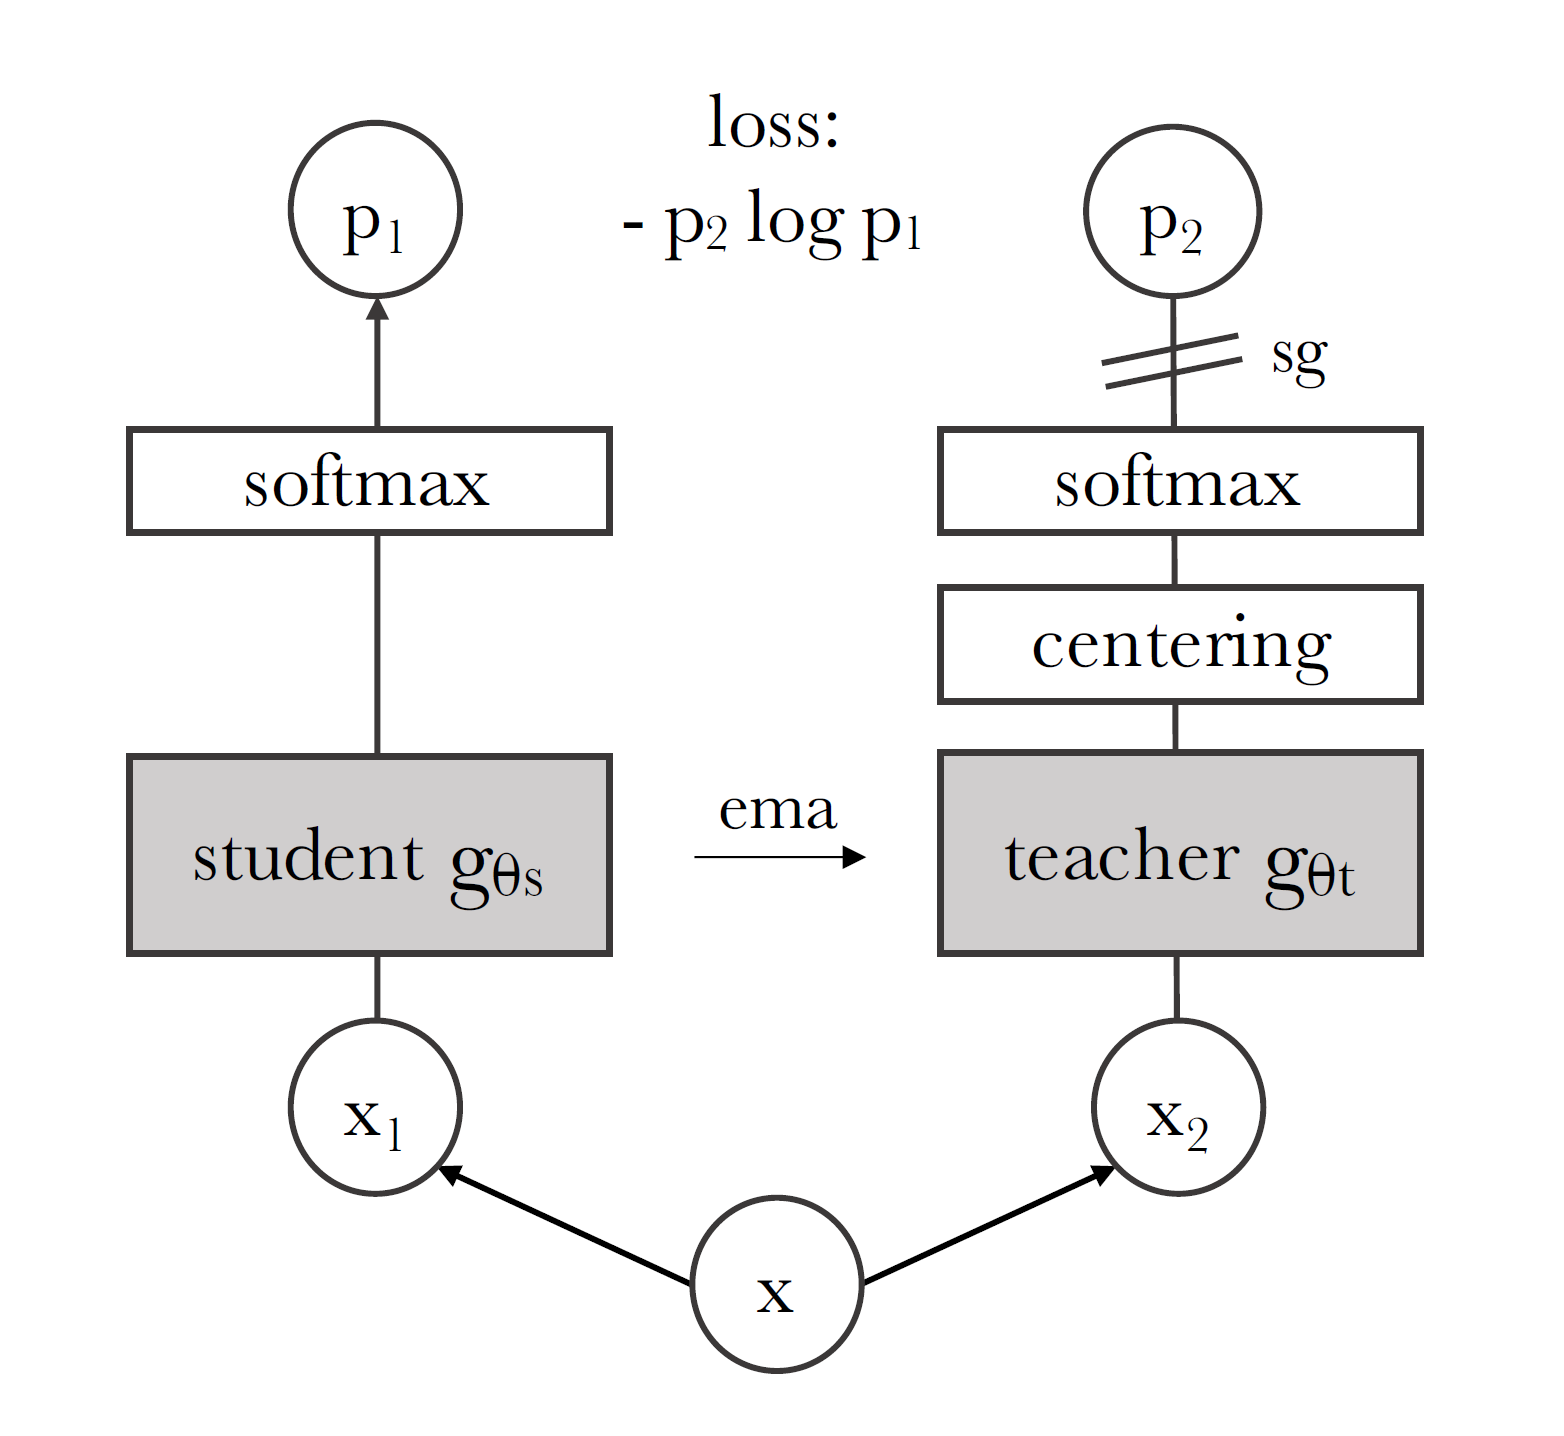
\includegraphics[width=0.5\textwidth]{Images_Thesis/dino_arch_v1.png}
\end{center}
\caption[Self Distillation with no labels]{ A diagram illustrating DINO with one image pair (x1, x2). The image undergoes two random transformations and is passed to both student and teacher networks, which have the same architecture but different parameters. The teacher's output is centered using the batch mean. Both outputs are normalized with temperature softmax and compared using cross-entropy loss. A stop-gradient operator is applied to the teacher, and its parameters are updated using an exponential moving average of the student's parameters~\citep{dino_caron2021emerging}.}
\label{fig:dino_v1_arch}
\end{figure}

The implementation of \gls{din}, as depicted in the figure~\ref{fig:dino_v1_arch}, employs two different random transformations of an input image, extracted from a single input image. These views are then processed by student and teacher networks, which have the same architecture but different parameters. The networks generate K-dimensional features that are normalized using a softmax function controlled by a temperature parameter. The similarity between these features is evaluated using cross-entropy loss. A stop-gradient operation is applied to the teacher to ensure that only the student is directly trained, enhancing the focus on feature generation without direct label dependence. For a comprehensive understanding of the implementation, interested readers can refer to section 3 of the DINO paper~\citep{dino_caron2021emerging}, which provides a complete mathematical foundation and explanation. This thesis focuses specifically on utilizing a pre-trained self-supervised vision transformer encoder to detect driver distraction on the \gls{daa} image dataset. The evaluation procedure used is a linear evaluation protocol.

The DINO architecture has significant implications for Vision Transformers~\citep{Vit_Paper_Dosovitskiy2020AnII} since it has the ability to provide novel qualities to \gls{vit}s, which have primarily been compared to classical \gls{cnn}s. The \gls{din} framework aims to assess the potential benefits of self-supervised \gls{vit}s, including the ability to explicitly describe semantic segmentation and perform successful k-NN classification directly from the features~\cite{dino_caron2021emerging}. In contrast to supervised \gls{vit}s and classical \gls{cnn}s, which do not naturally prioritize certain characteristics, DINO approach stands out and provides remarkable accuracy on ImageNet~\citep{Imagenet1k_ILSVRC15, Imagenet_21K_ridnik2021imagenet} dataset without the need for finetuning~\cite{dino_caron2021emerging}.

\paragraph{Self-Distillation with NO labels Version 2~(DINOv2):}
Building on the fundamental ideas of \gls{din}~\cite{dino_caron2021emerging}, the architecture and training technique are enhanced and refined in various ways in \gls{dino}~\cite{dinov2_oquab2023dinov2}. The architecture of \gls{dino} signifies a significant progression in self-supervised learning in the field of computer vision. It integrates discriminative learning techniques to enhance feature extraction and improve model performance. The \gls{dino} architecture is centered around a dual approach that consists of a student and a teacher network as introduced intially in the \gls{din} paper~\cite{dino_caron2021emerging}. This modified approach utilizes self-distillation techniques to promote strong feature learning without the need for labeled data~\cite{dinov2_oquab2023dinov2}.

The fundamental enhancements in the \gls{dino} architecture consist of:
\begin{itemize}
    \item \textbf{Discriminative Self-supervised Pre-training:}  \gls{dino} utilizes a novel combination of loss functions from \gls{din}~\cite{dino_caron2021emerging} and \gls{ibot}~\citep{_ibot_image_bert_zhou2021ibot}, integrated with the centering mechanism from \gls{swav}~\citep{_SwAV_caron2020unsupervised}. This configuration aids in stabilizing the feature space, preventing the trivial solutions often encountered in self-supervised learning scenarios~\citep{dinov2_oquab2023dinov2}.
    \item \textbf{Dual-Objective Learning:}
        \begin{itemize}
            \item \textbf{Image-level Objective~\cite{dino_caron2021emerging}:} At this level, \gls{dino} framework applies a cross-entropy loss between the outputs of the student and the teacher networks, derived from the class token of a Vision Transformer~\citep{Vit_Paper_Dosovitskiy2020AnII} model. The outputs are obtained from different crops of the same image, encouraging the model to recognize and learn consistent features across varied perspectives and scales~\citep{dino_caron2021emerging, dinov2_oquab2023dinov2}.
            \item \textbf{Patch-level Objective~\citep{_ibot_image_bert_zhou2021ibot}:} This objective introduces variability in the input by masking some patches presented to the student network, but not to the teacher. A cross-entropy loss is then computed between the patch features from both networks. This added complexity ensures the model captures detailed textural and structural information at finer granularities, thus enhancing its overall sensitivity to image content~\citep{dinov2_oquab2023dinov2}. 
        \end{itemize}
    \item \textbf{Adaptive Weight Management:} To optimize learning at different scales, \gls{dino} employs a strategy of untying the head weights for the image-level and patch-level objectives. This approach corrects the tendency of the model to underfit at the patch level or overfit at the image level, thereby balancing the learning focus and improving outcomes at both scales~\citep{dinov2_oquab2023dinov2}. 
    \item \textbf{Sinkhorn-Knopp Centering~\citep{_SwAV_caron2020unsupervised}:} The DINOv2 architecture adopts the Sinkhorn-Knopp (SK) algorithm for batch normalization~\citep{_SwAV_caron2020unsupervised} from \gls{swav} framework, a method initially suggested for the \gls{din} and \gls{ibot} framework by \citet{ruan2022weighted}. This algorithm, recommended for its efficiency in normalizing features, replaces the softmax centering typically used in DINO and iBOT setups~\citep{ruan2022weighted}. The SK centering is applied in three iterative steps, mainly for the teacher network, while the student employs softmax normalization. This element helps in maintaining a uniform distribution of features across batches, crucial for consistent self-supervised learning~\citep{dinov2_oquab2023dinov2}.
    \item \textbf{Regularization and High-Resolution Training Phase:} In addition to these structural components, \gls{dino} incorporates KoLeo regularizer~\citep{_koleo_sablayrolles2018spreading} to ensure a diverse spread of features across the learning process and introduces a short high-resolution training phase. These enhancements allow the model to adapt better to high-resolution tasks, which are particularly relevant in contexts such as detailed image analysis, segmentation, and object detection~\citep{dinov2_oquab2023dinov2}.
\end{itemize}

The primary distinctions between DINO and DINOv2 are outlined below:

\textbf{Loss Function Integration:}
    \begin{itemize}
        \item DINO: Introduced knowledge distillation emphasizing feature invariance across various perspectives of the same image~\citep{dino_caron2021emerging}.
        \item DINOv2: Integrated a combination of \gls{din} and \gls{ibot} loss functions, along with the centering techniques from \gls{swav}, to stabilize the learning process further~\citep{dinov2_oquab2023dinov2}.
    \end{itemize}
\textbf{Objective Functions:}
    \begin{itemize}
        \item DINO: Primarily focused on image-level objectives to encourage feature learning across different augmentations of input data~\citep{dino_caron2021emerging}.
        \item DINOv2: Introduced patch-level objectives alongside image-level objectives, involving masking some image patches for the student but not for the teacher, adding complexity and encouraging more detailed feature learning~\citep{dinov2_oquab2023dinov2}.
    \end{itemize}
\textbf{Weight Management:}
    \begin{itemize}
        \item DINO: Did not explicitly address weight tying between different objectives.
        \item DINOv2: Improved the architecture by untying the weights between image-level and patch-level objectives, enhancing model performance across different scales and preventing overfitting or underfitting~\citep{dinov2_oquab2023dinov2}.
    \end{itemize}


\paragraph{Evaluation Protocols for SSL Models}
The evaluation of self-supervised learning \gls{ssl} models, such as our DINOv2-based ViT encoder~\citep{dinov2_oquab2023dinov2}, deviates substantially from conventional supervised approaches. The methods of evaluation for \gls{ssl} models are essential for determining their effectiveness in downstream tasks like driver distraction detection, as these models are generally evaluated based on their capacity to generate valuable representations without direct supervision. 

\paragraph{Types of SSL Evaluation:}
\begin{enumerate}
    \item \textbf{K-Nearest Neighbors (KNN):}
    In the context of \gls{ssl}, a KNN classifier~\citep{kNN_Mucherino2009} uses $\displaystyle l_2$-normalized features extracted by the model to classify new images based on the closest training examples in feature space. This method is advantageous due to its simplicity, speed, and minimal hyperparameter tuning, making it an ideal quick benchmark for SSL models \citep{dino_caron2021emerging, ssl_codebook_balestriero2023cookbook}.

    \item \textbf{Linear Evaluation:}
    The most popular method for evaluating \gls{ssl} models is the linear evaluation, or linear probing. This method tests the quality of the backbone directly, as the linear classifier has limited capacity to adjust to the data, thereby providing a clear signal of the representational power of the underlying parameters. Typically, this involves appending a linear layer to the frozen backbone and optimizing it for several epochs (usually around 100), which is computationally efficient \citep{ssl_zhang_2016_colorful,ssl_zhang_2017split,ssl_codebook_balestriero2023cookbook,ssl_beit_bert_bao2021beit}.

    \item \textbf{Full Fine-Tuning:}
    This method involves training the entire model (both the pre-trained backbone and the newly added classifier) on a downstream task such as driver distraction detection. It is the most thorough evaluation, allowing the model to fully adapt to the new task. However, it is also the most computationally expensive and may not always correlate with the strength of the initial \gls{ssl} pre-training, especially in scenarios where the downstream task is substantially different from the pre-training setup \citep{masked_ae_he2021masked, ssl_codebook_balestriero2023cookbook}.

    \item \textbf{Multi-Layer Perceptron (MLP) Probing:}
    While less common, MLP probing involves adding a small multi-layer perceptron on top of the frozen features. This can reveal whether the features are non-linearly separable, which may be masked by simpler linear probing. However, this approach is more prone to overfitting and typically requires careful management of model capacity and training duration \citep{ssl_bordes2023towards, ssl_codebook_balestriero2023cookbook}.
\end{enumerate}

%%%%%%%%%%%%%%%%%%%%%%%% Chapter 4: Method %%%%%%%%%%%%%%%%%%%%
%%%%%%%%%%%%%%%%%%%%%%%%%%%%%%%%%%%%%%%%%%%%%%%%%%%%%%%%%%%%%%%%%%%
%%%%%%%%%%%%%%%%%%%%%%%%%%%%%%%%%%%%%%%%%%%%%%%%%%%%%%%%%%%%%%%%%%%
%%%%%%%%%%%%%%%%%%%%%%%%%%%%%%%%%%%%%%%%%%%%%%%%%%%%%%%%%%%%%%%%%%%
\chapter{Proposed Methods}
\label{chapter:proposed_methods}
In Chapter 3, we explored clustering, vision transformers, and self-supervised learning frameworks like DINO and DINOv2, including their evaluation in various scenarios. Building on that, Chapter 4 outlines our proposed methods and the steps involved in our experiments. We start with how we created our image datasets using annotation files provided for DAA video dataset, including addressing dataset imbalance and relevant statistics. We introduce a new dataloader designed specifically for imbalanced datasets and describe our clustering process. The chapter also explains our methodologies for comparing new dataloader with traditional one and training and evaluating our models. Additionally, we provide necessary mathematical formulations to aid in understanding our evaluation principles, and we outline our experimental goals, which will be tested in the following chapter.

\section{Image Dataset Generation}
This section explains how we created image datasets from the \gls{daa} video dataset~\citep{martin2019drive_and_act_2019_iccv} using the provided annotation files. First, we'll examine the structure of these annotation files to understand how to extract frames from the \gls{daa} videos. We'll then go over the data pre-processing steps and frame extraction process. By the end of this section, we'll have prepared the extracted image datasets for an analysis of any imbalances in the next section.

\paragraph{Dataset Annotation Details:} The annotation files are integral for indexing and extracting relevant frames. An example of such a file,~``midlevel.chunks\_90.split\_0.train.csv", provided by \gls{daa}~\citep{martin2019drive_and_act_2019_iccv} video dataset, is depicted in the figure~\ref{fig:example of an annotation file}. It includes headers like participant\_id, file\_id, annotation\_id, frame\_start, frame\_end, activity, and chunk\_id. For instance, entries in this file indicate specific activities such as `closing\_door\_outside' and `opening\_door\_outside', with precise frame ranges provided for effective localization of the activity within the video because each activity is captured for 3 seconds and corresponds to 1 video sample~\citep{martin2019drive_and_act_2019_iccv}.

\begin{figure}[h]
\begin{center}
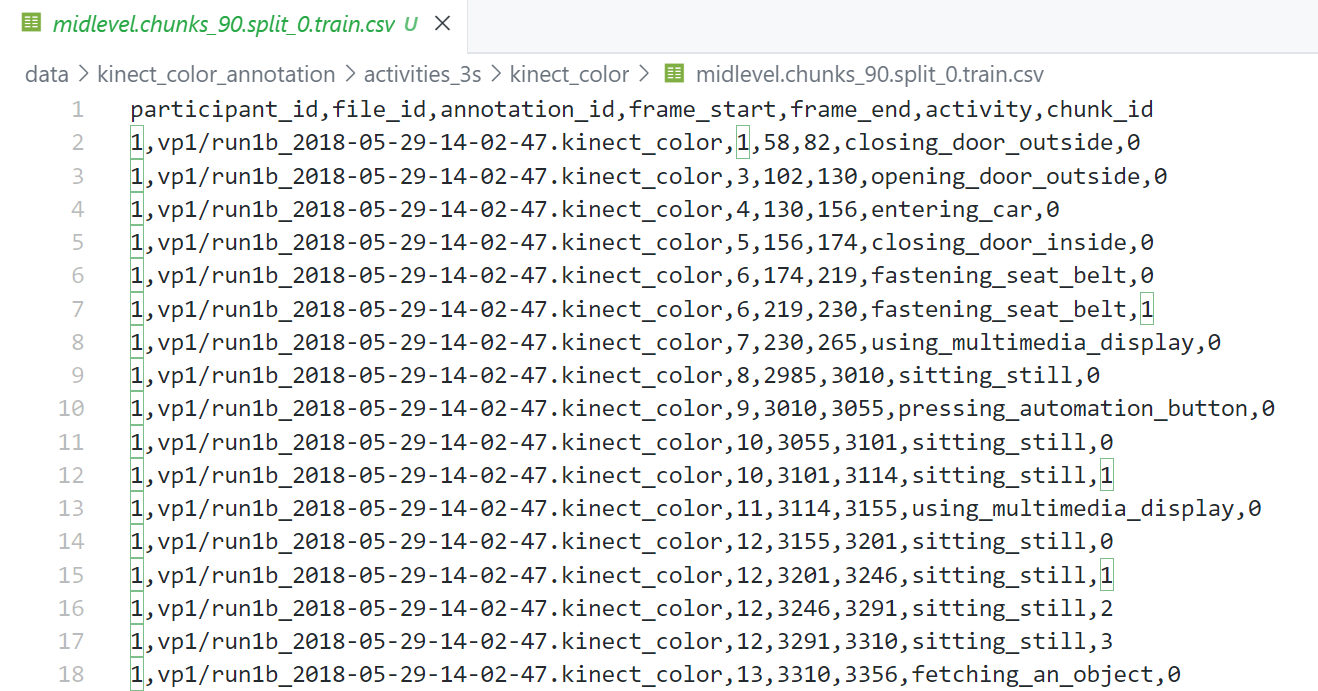
\includegraphics[width=0.8\textwidth]{Images_Thesis/annotation_example.png}
\end{center}
\caption[Example of an annotations file.]{This figure depicts the annotation structure in the ``midlevel.chunks\_90.split\_0.train.csv" file provided by~\citet{martin2019drive_and_act_2019_iccv} for the train dataset of the split 0 of the Kinect Color \gls{daa} video dataset.It includes headers like participant\_id, file\_id, annotation\_id, frame\_start, frame\_end, activity, and chunk\_id. These details are utilized to extract exact image frames corresponding to each activity in the \gls{daa} video dataset.}
\label{fig:example of an annotation file}
\end{figure}

\paragraph{Data Preprocessing and Frame Extraction:} The methodology's initial step involves extracting image frames from the video files of the \gls{daa} dataset. This process forms foundational image datasets corresponding to each considered modality and camera view. Table~\ref{table for views and modalities in daa dataset} contains information about different modalities and views offered by \gls{daa} dataset~\citet{martin2019drive_and_act_2019_iccv}. Specifically, two camera views are utilized for this research: the `Right Top View' and the `Front Top View' as depicted in the table~\ref{table for views and modalities used in this thesis}. Two `Right Top View' datasets come from color and infrared videos captured by the Kinect camera and one `Front-top View' dataset comes from NIR camera recordings. Table~\ref{table for different daa dataset versions formed in this thesis} lists the different image datasets obtained as a results of frame extraction procedure on the \gls{daa} video dataset. Additionally, it includes details regarding the specific perspective captured in the dataset, as well as the designated name for the image dataset within the context of this thesis. The number of channels in the table~\ref{table for different daa dataset versions formed in this thesis} includes information about the number of channels in each image, where for gray scale images there are 3 channels in which each channel contains the same information or in other words one gray scale channel is repeated thrice. This thesis focuses on training models using the `Kinect Right Top View' color \gls{daa} dataset and evaluating their performance on Infrared (Grayscale) datasets to assess their ability to generalize across different modalities and viewpoints.

\paragraph{Dataset Categorization:} This thesis focuses on driver distraction, which necessitates a streamlined approach to data categorization. The extracted drive and act image datasets, consisting of 34 distinct midlevel activities that detail various driver behaviors, are further reorganised into two main classes: `\_non\_distracted' and `distracted' driver. The `\_non\_distracted' class includes activities that indicate the driver's full attention to driving. For example, the `sitting\_still' activity is clearly aligned with a non-distracted state. Similarly, activities like `entering\_car' and `exiting\_car', which occur outside the active driving period, are also grouped under `non\_distracted'. Alternatively, these activities could be excluded altogether, allowing the analysis to focus strictly on a binary classification: `sitting\_still' versus all other activities. 

In contrast, the `distracted' class comprises the remaining 31 fine-grained activities depicted in figure~\ref{fig:driveandact_activities}, representing potential distractions from the driving task. This binary categorization simplifies the dataset, enhancing its compatibility with the PyTorch Image Folder class~\citep{torchvision_imagefolder}.

\begin{table}[t]
\caption[Different views and modalities in Drive and Act Dataset.]{Different views and modalities in Drive and Act Dataset. Source:~\citep{martin2019drive_and_act_2019_iccv}}
\label{table for views and modalities in daa dataset}
\begin{center}
\small
\begin{tabular}{lll}
\multicolumn{1}{c}{\bf Camera Type}  &\multicolumn{1}{c}{\bf Modality Type} &\multicolumn{1}{c}{\bf View Type}
\\ \hline 
NIR         & Infra-red (Gray scale)  &Front Top
\\ \hline
NIR         & Infra-red (Gray scale)  &Right Top
\\ \hline 
NIR         & Infra-red (Gray scale)  &Back
\\ \hline 
NIR         & Infra-red (Gray scale)  &Face view
\\ \hline 
NIR         & Infra-red (Gray scale)  &Left Top
\\ \hline 
Kinect         & Color (RGB)  &Right Top
\\ \hline 
Kinect         & Depth  &Right Top
\\ \hline 
Kinect        & Infra-red (Gray scale)  &Right Top
\\ \hline 
\end{tabular}
\end{center}
\end{table}

\begin{table}[t]
\caption[Different views and modalities from Drive and Act Dataset used in this thesis.]{Different views and modalities from Drive and Act Dataset used in this thesis. Source:~\citep{martin2019drive_and_act_2019_iccv}}
\label{table for views and modalities used in this thesis}
\begin{center}
\small
\begin{tabular}{lll}
\multicolumn{1}{c}{\bf Camera Type}  &\multicolumn{1}{c}{\bf Modality Type} &\multicolumn{1}{c}{\bf View Type}
\\ \hline 
NIR         & Infra-red (Gray scale)  &Front Top
\\ \hline 
Kinect         & Color (RGB)  &Right Top
\\ \hline 
Kinect        & Infra-red (Gray scale)  &Right Top
\\ \hline
\end{tabular}
\end{center}
\end{table}

\begin{table}[t]
\caption[Different version of Drive and Act (DAA) Image Datasets formed in this thesis.]{Different version of Drive and Act (DAA) Image Datasets formed in this thesis. Source:~\citep{martin2019drive_and_act_2019_iccv}}
\label{table for different daa dataset versions formed in this thesis}
\begin{center}
\small
\begin{tabular}{llll}
\multicolumn{1}{c}{\bf Camera and Modality Type}  &\multicolumn{1}{c}{\bf View Type} &\multicolumn{1}{c}{\bf Dataset Name} &\multicolumn{1}{c}{\bf Number of Channels}
\\ \hline 
Near Infra-red (Gray scale)  &Front Top & NIR Front Top Image DAA & 1 x 3 (duplicated)
\\ \hline 
Kinect Color (RGB)  &Right Top & Kinect Color Right Top Image DAA & 3 (RGB)
\\ \hline 
Kinect Infra-red (Gray scale)  &Right Top & Kinect IR Right Top Image DAA & 1 x 3 (duplicated)
\\ \hline
\end{tabular}
\end{center}
\end{table}

\subsection{Dataset Statistics}
\label{section:Imbalance and Dataset Statistics}
After extracting the image datasets into 34 fine grained activities, there is evidence of significant disparities in class distribution within the resulted image datasets.~Figure~\ref{fig:driveandact_multi_class_imbalance_split_0} illustrates the disparities among the 34 fine-grained activities in `split 0' of the `Kincet Color Right Top Image DAA' train dataset. The dataset for this split contains a total of 259,865 images. Of these, the `sitting\_still' class alone comprises 78,227 images, which account for 30.10\% of the dataset. This starkly contrasts with categories such as `closing\_door\_outside,' which represents a mere 0.087\% with only 226 images. Such imbalances highlight the challenges in training models that can accurately recognize less frequent activities. However, this view gives us multi-class classification perspective of the image datasets and we need to further analyse the statistics for the binary classification task `non distracted' driver versus `distracted' driver. The imbalance ratio~\citep{23_ImR_buda2018systematic} is used as a standard metric to calculate the imbalance with respect to minority and majority classes rather than class ratios with respect to whole dataset size.
%%%%%%%%%%%%%%%%%%%%%%%%%%%%%%%%%%%%%%%%%%%%%%%%%%%%%%%%%%%%%%%%
%%%%%%%%%%% Class ratios figure split_0 Color DAA %%%%%%%%%%%%
\begin{figure}[h]
\begin{center}
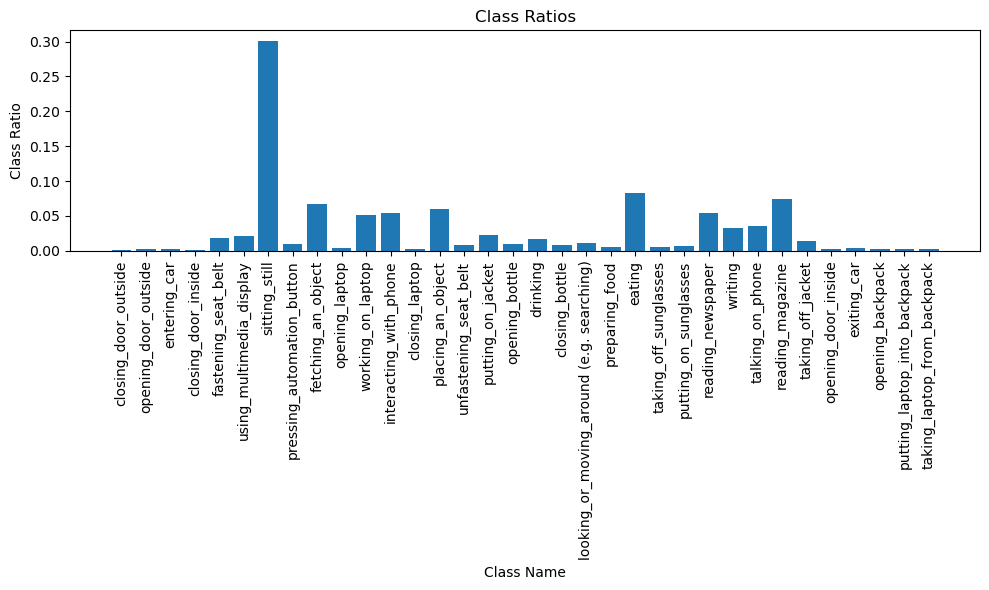
\includegraphics[width=0.8\textwidth]{Images_Thesis/daa_images/class_ratios_spli_0_train_output.png}
\end{center}
\caption[Illustrative image depicting the class imbalance in the split 0 of the Kincet Color Right Top Image DAA train dataset with 34 fine grained activities.]{Illustrative image depicting the class imbalance in the split 0 of the Kincet Color right Top Image DAA train dataset with 34 fine grained activities. The y-axis represents the class ratios and the x-axis represents 34 fine-grained activities. This extracted image dataset can be used for multi-class classification tasks like driver action recognition.}
\label{fig:driveandact_multi_class_imbalance_split_0}
\end{figure}

\paragraph{Method to calculate the class ratios}
Suppose we have a dataset with 34 distinct classes. Let \( N \) be the total number of images in the train set of split 0 of the `Kinect Color Right Top \gls{daa}' dataset, and let \( N_i \) be the number of images in each class \( C_i \) for \( i = 1, 2, \ldots, 34 \).

The class ratio \( R_i \) for each class \( C_i \) with respect to the total dataset is defined as:
\begin{equation}
\begin{aligned}
R_i = \frac{N_i}{N}
\end{aligned}
\label{equation:4.1}
\end{equation}
which gives the proportion of elements in each class relative to the entire dataset~\citep{Survey_DL_Taghi_article, 23_ImR_buda2018systematic}.

To convert this class ratio into a proportional percentage, which expresses the proportion of each class as a percentage of the total dataset, we multiply the class ratio by 100~\citep{book_stat_ratios_bennett2003statistical}. Thus, the proportional percentage \( P_i \) is defined as:
\begin{equation}
\begin{aligned}
P_i = R_i \times 100
\end{aligned}
\label{equation:4.2}
\end{equation}
This provides the percentage of the dataset that belongs to each class, facilitating easier comparison and visualization of class distribution.

Furthermore, for any two different classes \( C_i \) and \( C_j \) with \( N_i \) and \( N_j \) denoting the number of elements in each class , the pairwise class ratio \( R_{ij} \) can be defined as:
\begin{equation}
\begin{aligned}
R_{ij} = \frac{N_i}{N_j}
\end{aligned}
\label{equation:4.3}
\end{equation}
which compares the relative sizes of any two classes.

For example, the class ratio for `sitting\_still' class can be calculated as follows:
\[
R_i = \frac{78227}{259865} = 0.3010
\]
And, the proportional percentage for `sitting\_still' class can be calculated as follows:
\[
P_i = 0.3010 \times 100 = 30.10\%
\]

\subsection{Imbalance Across Different Splits and Classes}

The datasets further contains the imbalance between `\_non-distracted' and `distracted' driver classes across each dataset split. Figure~\ref{fig:Class_dist_whole_grid_Kinect_color} shows the distribution of `\_non-distracted' and `distracted' driver classes in the Kinect color Right Top Image DAA Dataset. Tables~\ref{kir imbalance-table} to~\ref{nir imbalance-table}, presents the imbalance ratio (ImR) for all generated image datasets. The Imbalance Ratio (ImR) is the ratio of image count for the majority class (`distracted') to the image count for the minority class (`non-distracted')~\citep{Survey_DL_Taghi_article, 23_ImR_buda2018systematic}. This metric shows the significant skew in data distribution, affecting the training and performance of detection models.

For a binary classification dataset, mathematically, the Imbalance Ratio can be written as follows:
\begin{equation}
\begin{aligned}
ImR = \frac{N_{Majority}}{N_{Minority}}
\end{aligned}
\label{equation:4.4}
\end{equation}
where \(N_{Majority}\) represents the total number of images in the majority class and \(N_{Minority}\) represents the total number of images in the minority class~\citep{Survey_DL_Taghi_article, 23_ImR_buda2018systematic}.

%%%%%%%%%%%%%%%%%%%%%%%%%%%%%%%%%%%%%%%%%%%%%%%%%%%%%%%%%%%%%%%%
%%%%%%%%%%% Tables for Imabalnced Ratio %%%%%%%%%%%%
\begin{table}[htbp]
\caption{Imbalance in Kinect Color Right Top Image DAA Dataset}
\label{rgb imbalance-table}
\begin{center}
\small
\begin{tabular}{llllll}
\multicolumn{1}{c}{\bf Dataset Split}  &\multicolumn{1}{c}{\bf Modality} &\multicolumn{1}{c}{\bf View} &\multicolumn{1}{c}{\bf ImR Train} &\multicolumn{1}{c}{\bf ImR Validation} &\multicolumn{1}{c}{\bf ImR Test}
\\ \hline \\
Split\_0         &Kinect RGB  &Right Top  &$\frac{179931}{79934} = 2.25$ & $\frac{43703}{12321} = 3.54$ & $\frac{55930}{31385} = 1.78$  \\
\\ \hline \\
Split\_1             &Kinect RGB  &Right Top  &$\frac{190562}{94245} = 2.02$ & $\frac{37934}{16607} = 2.28$ & $\frac{51068}{12788} = 3.99$ \\
\\ \hline \\
Split\_2             &Kinect RGB & Right Top & $\frac{188635}{73101} = 2.58$ & $\frac{34274}{19638} = 1.74$ & $\frac{56655}{30901} = 1.83$\\
\\ \hline
\end{tabular}
\end{center}
\end{table}

%%%%%%%%%%%%%%%%%%%%%%%%%%%%%%%%%%%%%%%%%%%%%%%%%%%%%%%%%%%%%%%%%
\begin{table}[htbp]
\caption{Imbalance in Kinect IR Right Top Image DAA Dataset}
\label{kir imbalance-table}
\begin{center}
\small
\begin{tabular}{llllll}
\multicolumn{1}{c}{\bf Dataset Split}  &\multicolumn{1}{c}{\bf Modality} &\multicolumn{1}{c}{\bf View} &\multicolumn{1}{c}{\bf ImR Train} &\multicolumn{1}{c}{\bf ImR Validation} &\multicolumn{1}{c}{\bf ImR Test}
\\ \hline \\
Split\_0         &Kinect Infra Red  &Right Top  & $\frac{209827}{87758} = 2.39$ & $\frac{50465}{13721} = 3.67$ & $\frac{64799}{34347} = 1.88$ \\
\\ \hline \\
Split\_1             &Kinect Infra Red  &Right Top  & $\frac{221575}{103027} = 2.15$ & $\frac{44258}{18448} = 2.399$ & $\frac{59258}{14351} = 4.129$ \\
\\ \hline \\
Split\_2             &Kinect Infra Red & Right Top & $\frac{218780}{80867} = 2.70$ & $\frac{40313}{21490} = 1.87$ & $\frac{65998}{33469} = 1.97$  \\
\\ \hline
\end{tabular}
\end{center}
\end{table}

%%%%%%%%%%%%%%%%%%%%%%%%%%%%%%%%%%%%%%%%%%%%%%%%%%%%%%%%%%%%%%%
\begin{table}[htbp]
\caption{Imbalance in Near Infra Red Front Top Image DAA Dataset}
\label{nir imbalance-table}
\begin{center}
\small
\begin{tabular}{llllll}
\multicolumn{1}{c}{\bf Dataset Split}  &\multicolumn{1}{c}{\bf Modality} &\multicolumn{1}{c}{\bf View} &\multicolumn{1}{c}{\bf ImR Train} &\multicolumn{1}{c}{\bf ImR Validation} &\multicolumn{1}{c}{\bf ImR Test}
\\ \hline \\
Split\_0         &Near Infra Red  &Front Top  & $\frac{351345}{156522} = 2.24$ & $\frac{85400}{24101} = 3.54$ & $\frac{109493}{61492} = 1.78$ \\
\\ \hline \\
Split\_1             &Near Infra Red  &Front Top & $\frac{371987}{184436} = 2.01$ & $\frac{74304}{32598} = 2.27$ & $\frac{99947}{25081} = 3.98$ \\
\\ \hline \\
Split\_2             &Near Infra Red & Front Top & $\frac{369144}{143272} = 2.57$ & $\frac{67123}{38541} = 1.74$ & $\frac{109971}{60302} = 1.82$  \\
\\ \hline
\end{tabular}
\end{center}
\end{table}

%%%%%%%%%%%%%%%%%% Grid of class distributions %%%%%%%%%%%%%%%%%
\begin{figure}[htbp]
    \centering
    % First row
    \begin{subfigure}[b]{0.45\textwidth}
        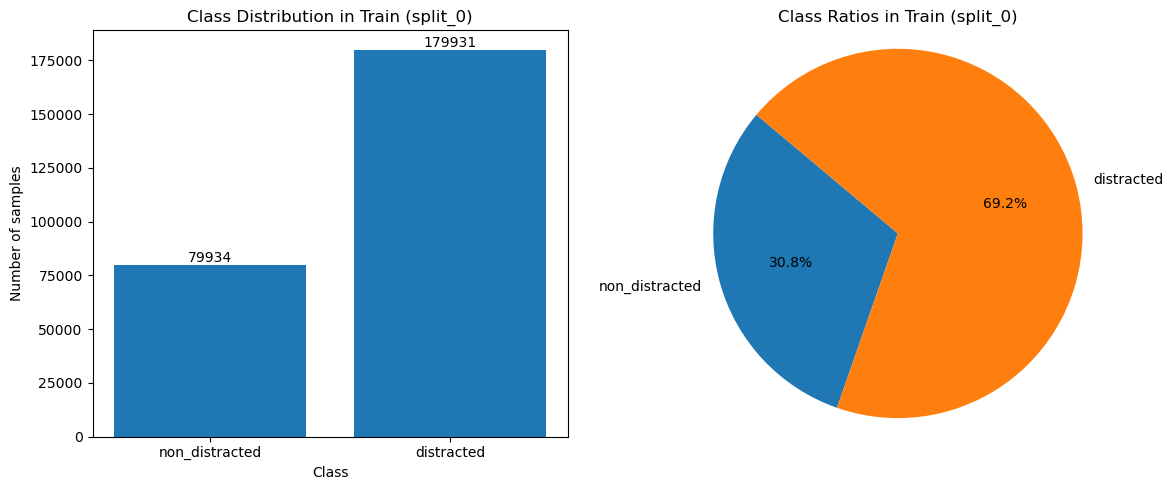
\includegraphics[width=\textwidth]{Images_Thesis/class_distribution_Kinect_color/split_0_rgb_daa/class_dist_train_sp_0_rgb_daa.png}
        \caption{Split 0: Train}
        \label{fig:Class_dist_grid_image1}
    \end{subfigure}
    \hfill % space between images
    \begin{subfigure}[b]{0.45\textwidth}
        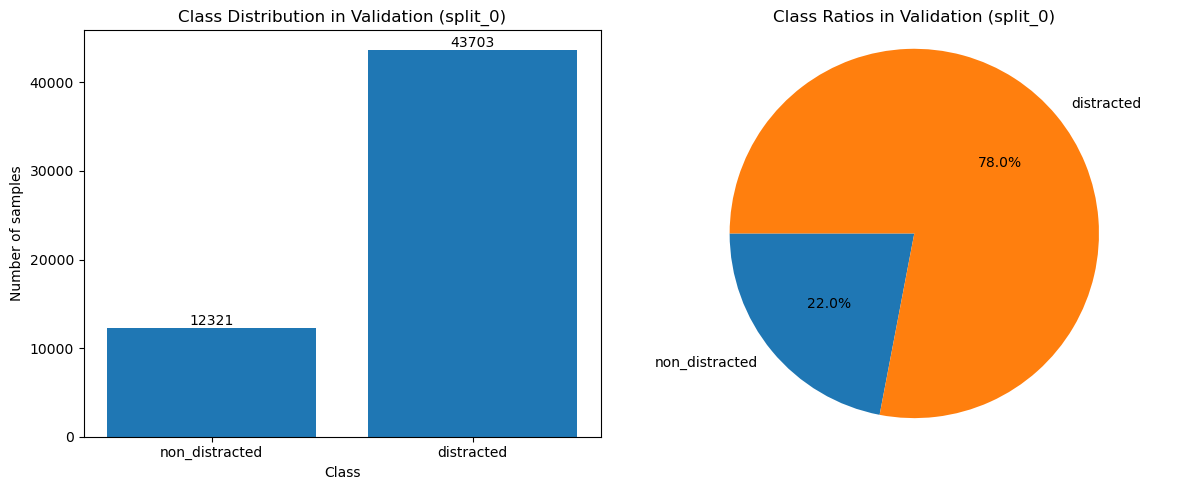
\includegraphics[width=\textwidth]{Images_Thesis/class_distribution_Kinect_color/split_0_rgb_daa/class_dist_val_sp_0_rgb_daa.png}
        \caption{Split 0: Validation}
        \label{fig:Class_dist_grid_image2}
    \end{subfigure}

    % Second row
    \begin{subfigure}[b]{0.45\textwidth}
        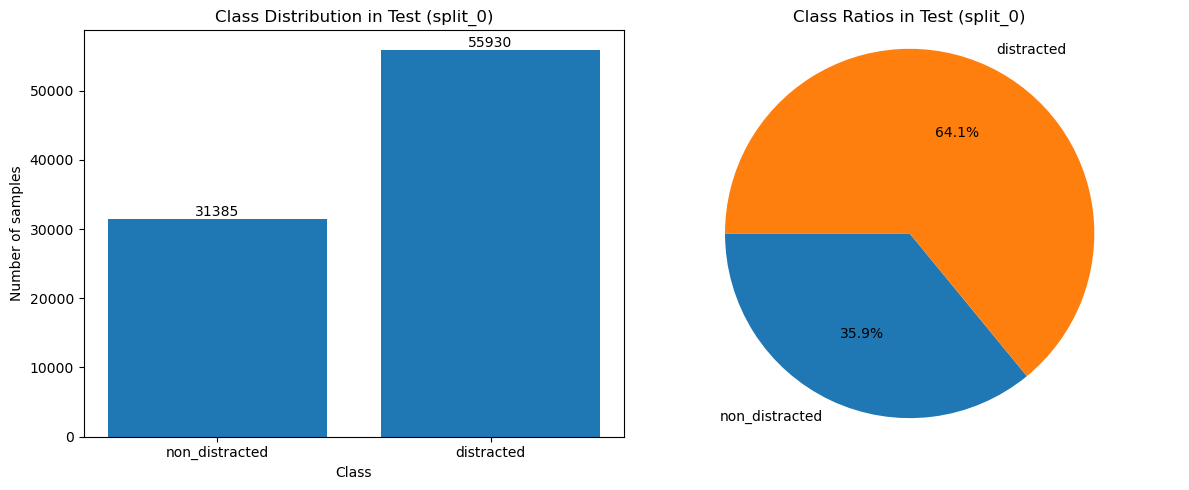
\includegraphics[width=\textwidth]{Images_Thesis/class_distribution_Kinect_color/split_0_rgb_daa/class_dist_test_sp_0_rgb_daa.png}
        \caption{Split 0: Test}
        \label{fig:Class_dist_grid_image3}
    \end{subfigure}
    \hfill
    \begin{subfigure}[b]{0.45\textwidth}
        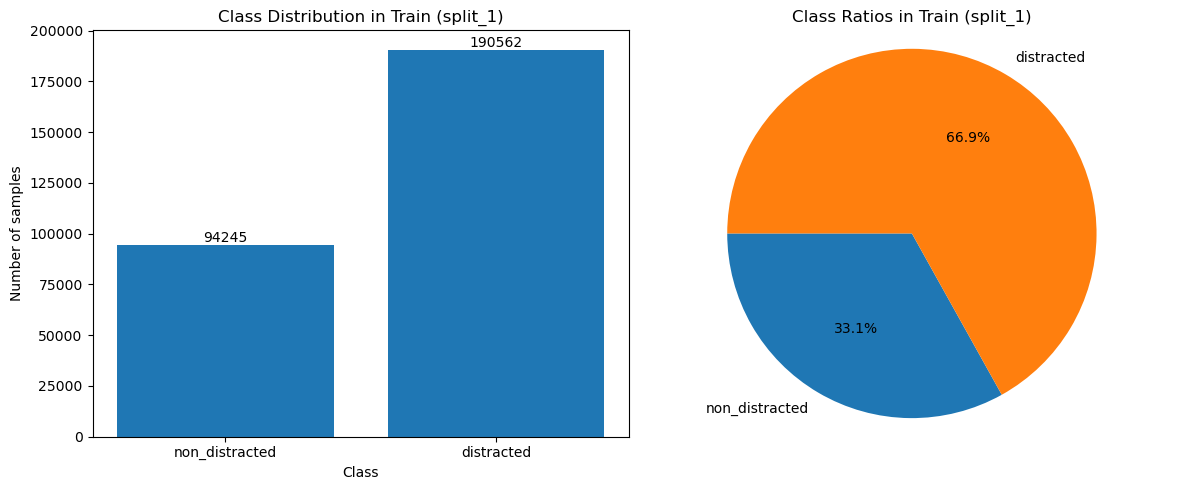
\includegraphics[width=\textwidth]{Images_Thesis/class_distribution_Kinect_color/split_1_rgb_daa/class_dist_train_rgb_sp_1_daa.png}
        \caption{Split 1: Train}
        \label{fig:Class_dist_grid_image4}
    \end{subfigure}

    % Third row
    \begin{subfigure}[b]{0.45\textwidth}
        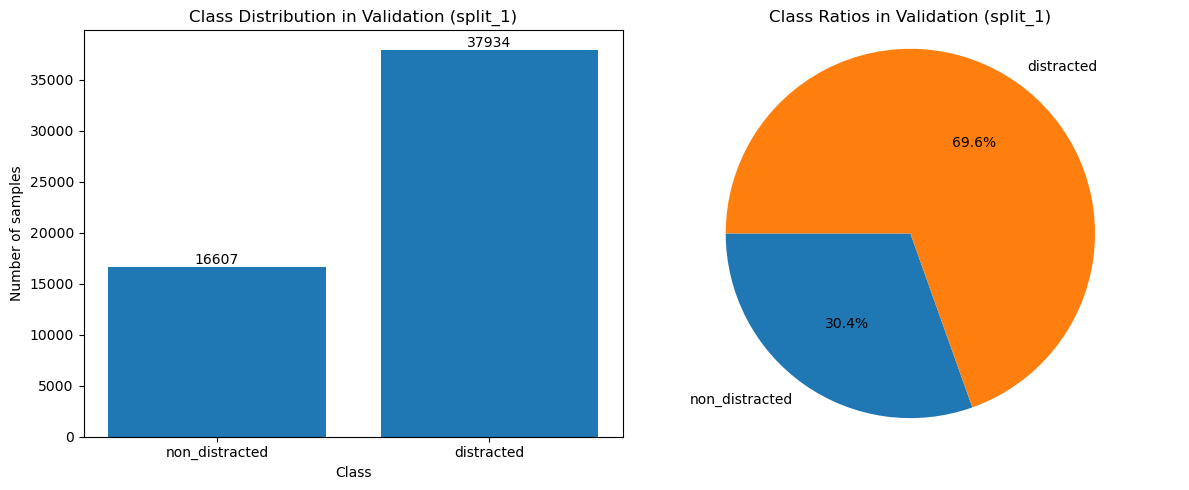
\includegraphics[width=\textwidth]{Images_Thesis/class_distribution_Kinect_color/split_1_rgb_daa/class_dist_val_sp_1_rgb_daa.png}
        \caption{Split 1: Validation}
        \label{fig:Class_dist_grid_image5}
    \end{subfigure}
    \hfill
    \begin{subfigure}[b]{0.45\textwidth}
        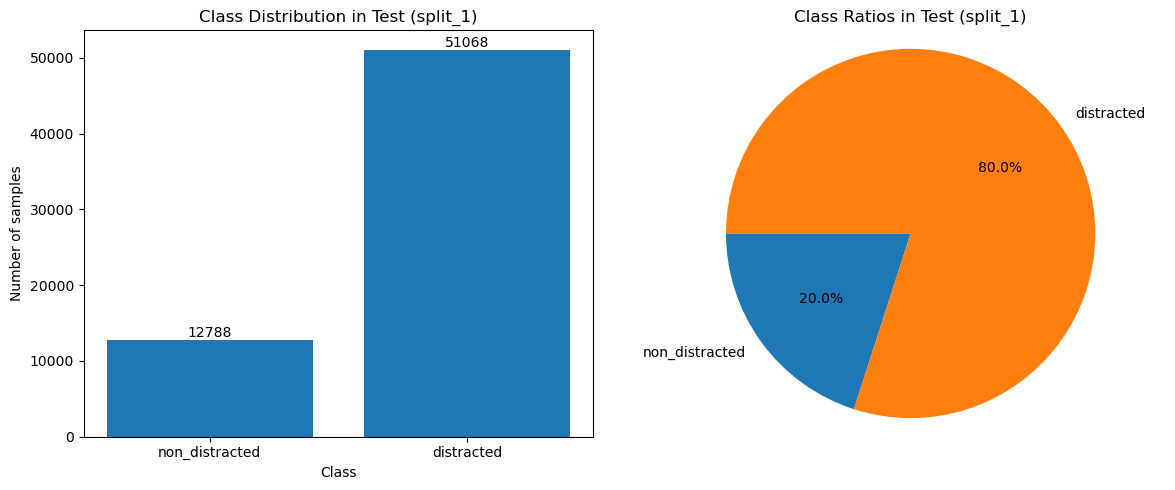
\includegraphics[width=\textwidth]{Images_Thesis/class_distribution_Kinect_color/split_1_rgb_daa/class_dist_test_sp_1_rgb_daa.png}
        \caption{Split 1: Test}
        \label{fig:Class_dist_grid_image6}
    \end{subfigure}

    % Fourth row
    \begin{subfigure}[b]{0.45\textwidth}
        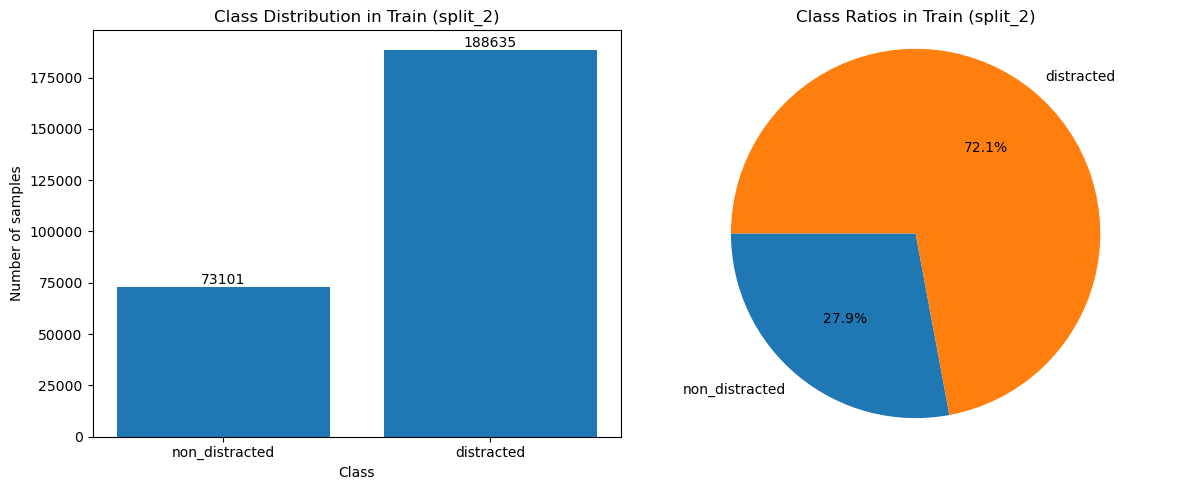
\includegraphics[width=\textwidth]{Images_Thesis/class_distribution_Kinect_color/split_2_rgb_daa/class_dist_train_sp_2_rgb_daa.png}
        \caption{Split 2: Train}
        \label{fig:Class_dist_grid_image7}
    \end{subfigure}
    \hfill
    \begin{subfigure}[b]{0.45\textwidth}
        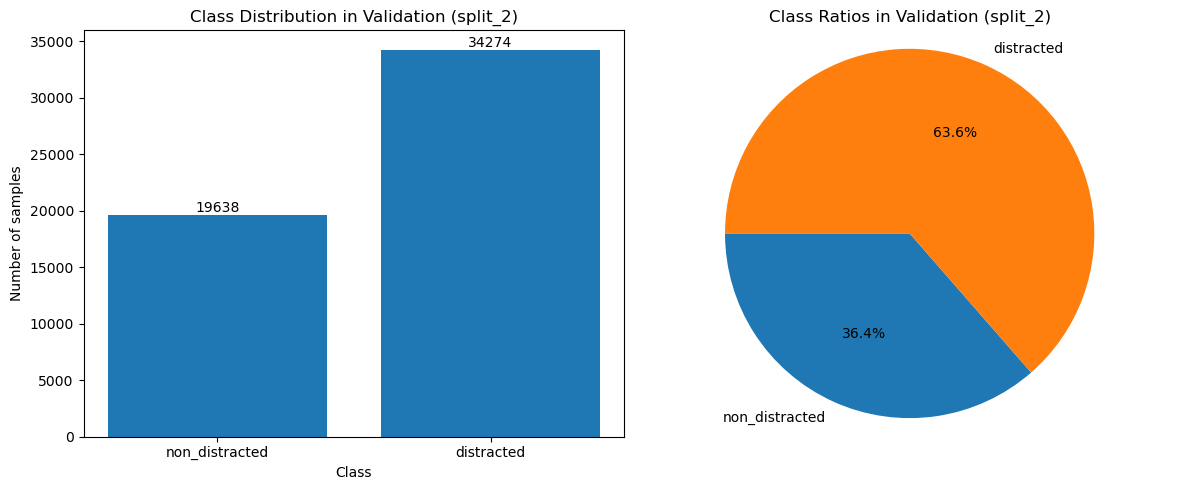
\includegraphics[width=\textwidth]{Images_Thesis/class_distribution_Kinect_color/split_2_rgb_daa/class_dist_val_sp_2_rgb_daa.png}
        \caption{Split 2: Validation}
        \label{fig:Class_dist_grid_image8}
    \end{subfigure}

    % Fifth row
    \begin{subfigure}[b]{0.45\textwidth}
        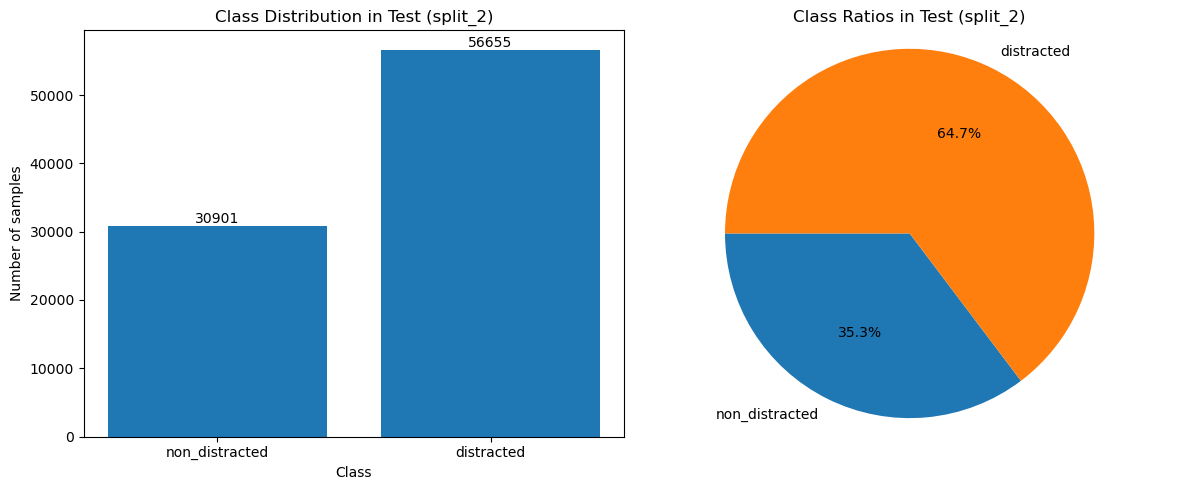
\includegraphics[width=\textwidth]{Images_Thesis/class_distribution_Kinect_color/split_2_rgb_daa/class_dist_test_sp_2_rgb_daa.png}
        \caption{Split 2: Test}
        \label{fig:Class_dist_grid_image9}
    \end{subfigure}

    \caption[Class distribution of all three splits of Kinect Color Right Top Image DAA Dataset.]{Class distribution of all three splits of Kinect Color Right Top Image DAA Dataset. In the bar plot, the x-axis corresponds to the class, while the y-axis reflects the number of images in each class. The pie chart displays the relative proportion, expressed as a percentage, of each class inside each split of the dataset. These proportions are generated based on the class ratios.}
    \label{fig:Class_dist_whole_grid_Kinect_color}
\end{figure}

\subsection{Proposed Evaluation Metrics}
As we have imbalance in the extracted image datasets, we can no longer rely on the traditional evaluation metrics like accuracy as already discussed in the chapter~\ref{chapter:related_work}. Accuracy is the ratio of correctly predicted observations to the total observations. It can be misleading in evaluating performance of a model on our imbalanced datasets. So, following the recommendations of~\citet{Survey_DL_Taghi_article, 18_wang2016training}, this thesis employs the balanced accuracy score instead of the standard accuracy score for evaluating model performance. Such metrics offer a more nuanced insight into how well models perform across all classes, irrespective of their frequency. Below is the definition and mathematical formulation of the balanced accuracy score. 

\paragraph{Balanced Accuracy:}
It is the average of the recall obtained on each class, ensuring equal treatment of each class's performance~\citep{bal_acc_paper_brodersen2010balanced, bal_acc_2_sk_learn_kelleher2015fundamentals}. 

For a binary classification problem with classes \( C_1 \) and \( C_2 \), where \( C_1 \) is considered the positive or minority class and \( C_2 \) the negative or majority class, the balanced accuracy can be mathematically expressed as follows:

Let:
\begin{itemize}
    \item \( TP \) denote the number of true positives.
    \item \( TN \) denote the number of true negatives.
    \item \( FP \) denote the number of false positives.
    \item \( FN \) denote the number of false negatives.
\end{itemize}

The recall for class \( C_1 \) (True Positive Rate) is:
\begin{equation}
\begin{aligned}
\text{Recall}_{C_1} = \frac{TP}{TP + FN}
\end{aligned}
\label{equation:4.5}
\end{equation}

The recall for class \( C_2 \) (True Negative Rate) is:
\begin{equation}
\begin{aligned}
\text{Recall}_{C_2} = \frac{TN}{TN + FP}
\end{aligned}
\label{equation:4.6}
\end{equation}

Therefore, the balanced accuracy is given by:
\begin{equation}
\begin{aligned}
\text{Balanced Accuracy} = \frac{\text{Recall}_{C_1} + \text{Recall}_{C_2}}{2}
\end{aligned}
\label{equation:4.7}
\end{equation}

With respect to this thesis, class \( C_1 \) represents the `\_non\_distracted' driver class whereas class \(C_2\) represents the `distracted' driver class. This formula ensures that both classes are equally represented in the accuracy metric, which is particularly important in cases of class imbalance~\citep{Survey_DL_Taghi_article, 18_wang2016training}.

\section{Novel Dataloader for Imbalanced Dataset}
To address the first research question of this thesis, we propose `Clustered Feature Weighting' a data loading strategy to improve imbalance in batches during model training. The methodology opted for the novel data loading is depicted in the flowchart~\ref{flowchart:flowchart_novel_dataloader_imbalanced_dataset}. This flowchart shows the step by step procedure opted for the creation of the novel dataloader titled ``ClusteredFeatureWeighting". The novel dataloader designed for this thesis aims to address the inherent bias towards the majority class in imbalanced datasets by introducing balanced batches during model training. This enhancement not only aims to mitigate model bias but also aims to improve model performance by feeding balanced batches during model training.

\subsection{Methodological Steps}
The methodology is divided into four main parts starting from model selection to final dataloader comparison as shown below. Each part of the methodology contains different design choices and verification procedures. First we will start with the explanation of the steps involved in implementing the novel dataloader, which are as follows:

\begin{enumerate}
    \item \textbf{Model Selection}: Choose a vision transformer model or encoder that has been pre-trained on the ImageNet-21K~\citep{Imagenet1k_ILSVRC15} dataset in order to obtain embeddings from the Kinect Right Top Color Drive and Act image dataset.
    
    \item \textbf{Variance Analysis}: Perform variance analysis on the collected features to assess the suitability of the selected model for feature extraction. Understanding the degree of separation between features within the same class and across different classes in the feature space is highly important. If the model is compatible with the imbalanced dataset under consideration, then move on to next step else select a suitable encoder again and verify its compatibility with the dataset under consideration by repeating the variance analysis. 
    \item \textbf{Clustering}: Arrange the features batchwise and Apply HDBSCAN~\citep{HDBSCAN_algo_campello2013density} clustering algorithm on the cosine distance between the extracted features batchwise. This step is explained in detail in the section~\ref{section:ClusteredFeatureWeighting Data Loading Strategy}.
    \item \textbf{Weight Generation}: Generate weights for a weighted random sampler based on the clustering results, to ensure diverse and representative samples in each batch.
    \item \textbf{Comparison}: Compare the effectiveness of the novel dataloader with traditional dataloader to validate improvements in batchwise imbalance. If the results are satisfactory then move on to model training or else try different weights for outliers in order to see its impact on the sampling and imbalance in batches.
\end{enumerate}

Before progressing with the methodological steps of the novel dataloader, it is essential to first establish the mathematical formulations that underpin these processes. These formulations not only guide the development and implementation of the dataloader but also serve as critical verification procedures for evaluating the efficacy of the selected model.

\begin{figure}[htbp]
\begin{center}
\tikzstyle{startstop} = [circle, 
minimum width=1cm, 
minimum height=1cm,
text centered, 
draw=black, 
fill=red!30]

\tikzstyle{io} = [trapezium, 
trapezium stretches=true, % A later addition
trapezium left angle=70, 
trapezium right angle=110, 
minimum width=3cm, 
minimum height=0.5cm, text centered, 
draw=black, fill=blue!20]

\tikzstyle{process} = [rectangle, 
minimum width=2cm, 
minimum height=0.5cm, 
text centered, 
text width=5cm, 
draw=black, 
fill=orange!20]

\tikzstyle{decision} = [diamond, 
minimum width=3cm, 
minimum height=2cm, 
text centered, 
draw=black, 
fill=green!20]
\tikzstyle{arrow} = [thick,->,>=stealth]

\begin{tikzpicture}[node distance=1.1cm]

\node (start) [startstop] {Start};
\node (in1) [io, below of=start] {Choose Encoder and do Feature Extraction};
\node (pro1) [process, below of=in1] {Perform Variance Analysis};
\node (dec1) [decision, below of=pro1, yshift=-1.5cm] {Model Compatibility};
\node (pro2a) [process, below of=dec1, yshift=-1.8cm] {Perform Clustering};
\node (pro2b) [process, right of=dec1, xshift=4.0cm] {Use Another Suitable Encoder};
\node (out1) [io, below of=pro2a] {Generate Weights};
\node (out2) [io, below of=out1] {Dataloader Comparison};
\node (dec2) [decision, below of=out2, yshift=-1.5cm] {Balanced Batches};
\node (pro3a) [process, below of=dec2, yshift=-1.5cm] {Model Training};
\node (pro3b) [process, right of=dec2, xshift=4.0cm] {Try different weights for Outliers};
\node (stop) [startstop, below of=pro3a] {Stop};

\draw [arrow] (start) -- (in1);
\draw [arrow] (in1) -- (pro1);
\draw [arrow] (pro1) -- (dec1);
\draw [arrow] (dec1) -- node[anchor=east] {Yes} (pro2a);
\draw [arrow] (dec1) -- node[anchor=south] {No} (pro2b);
\draw [arrow] (pro2b) |- (pro1);
\draw [arrow] (pro2a) -- (out1);
\draw [arrow] (out1) -- (out2);
\draw [arrow] (out2) -- (dec2);
\draw [arrow] (dec2) -- node[anchor=east] {Yes} (pro3a);
\draw [arrow] (dec2) -- node[anchor=south] {No} (pro3b);
\draw [arrow] (pro3b) |- (pro2a);
\draw [arrow] (pro3a) -- (stop);

\end{tikzpicture}
\end{center}
\caption{Methodology for Novel Dataloader for Imbalanced Dataset.}
\label{flowchart:flowchart_novel_dataloader_imbalanced_dataset}
\end{figure}

\paragraph{Mathematical Definitions and Formulations:}
To quantitatively analyze the features extracted by a model, several mathematical measures are employed. These measures are pivotal for evaluating how well a model can capture and differentiate features within and between different classes, which directly impacts the effectiveness of classification algorithms and in our case the novel dataloading startegy.

\paragraph{Intra-class Variance} (\(\sigma_{intra}^2\)):
Intra-class variance quantifies the variability or spread of feature vectors within a single class. It measures how much the features of individual samples deviate from the mean feature vector of their respective class. A lower intra-class variance indicates a high degree of similarity among the samples within the class, suggesting that the model is consistent in capturing features for a specific class~\citep{intra_class_var_pilarczyk2019intra}.

Mathematically,
\begin{equation}
\begin{aligned}
\sigma_{intra}^2 = \frac{1}{N} \sum_{i=1}^N (\vx_i - \mu)^2
\end{aligned}
\label{equation:4.8}
\end{equation}
where: \( \vx_i \) represents the feature vector of the \(i\)-th image in a class, \( \mu \) denotes the mean feature vector of that class, and \( N \) is the total number of samples in the class~\citep{intra_class_var_pilarczyk2019intra}.

\paragraph{Calculation of Class Centers:}
To calculate the class centers in a feature space extracted using a pretrained Vision Transformer model, the mean feature vector (center) for each class is computed by averaging the feature vectors of all samples within each class~\citep{intra_class_var_pilarczyk2019intra}. As there are two classes (A) `non\_distracted' and (B) distracted in the dataset under consideration, we can calculate the class centers for each class in the feature space as follows: 
If $\displaystyle N$ is the total number of sample in each class, then,

For class A:
\begin{equation}
\begin{aligned}
\text{center}_A = \text{Mean Feature Vector}_A = \mu_0 = \frac{1}{\displaystyle N} \sum_{i=1}^{\displaystyle N} \displaystyle \vx_i^A
\end{aligned}
\label{equation:4.9}
\end{equation}
where $\displaystyle \vx_i^A$ represents the feature vector of the $i$-th sample in class A.

For class B:
\begin{equation}
\begin{aligned}
\text{center}_B = \text{Mean Feature Vector}_B = \mu_1 = \frac{1}{\displaystyle N} \sum_{i=1}^{\displaystyle N} \displaystyle \vx_i^B
\end{aligned}
\label{equation:4.10}
\end{equation}
where $\displaystyle \vx_i^B$ represents the feature vector of the $i$-th sample in class B.

\paragraph{Inter-class Variance} (\(\sigma_{inter}^2\)):
Inter-class variance measures the differences between the mean feature vectors of different classes. This metric is crucial for determining how distinct the classes are from each other in the feature space. Higher values of inter-class variance suggest that the classes are more distinguishable, indicating that the model is effective in capturing diverse features necessary for differentiating between classes~\citep{inter_class_yu2022generalized}.
Mathematically,
\begin{equation}
\begin{aligned}
\sigma_{inter}^2 = (\mu_0 - \mu_1)^2
\end{aligned}
\label{equation:4.11}
\end{equation}
where: \( \mu_0 \) and \( \mu_1 \) are the mean feature vectors of two different classes.

\paragraph{Distance Between Class Centers:}
The distance between class centers is an additional metric used to evaluate the separability of classes within the feature space. This measure complements inter-class variance by providing a direct assessment of the spatial separation between class centers, which can be interpreted as an indicator of the model’s ability to partition the feature space effectively. Once the centers of each class are computed, the Euclidean distance~\citep{wikipedia_euclidean_distance} between these two centers can be calculated using the following formula:

\begin{equation}
\begin{aligned}
d(\text{center}_A, \text{center}_B) = \sqrt{\sum_{i=1}^{\displaystyle M} (\text{center}_A[i] - \text{center}_B[i])^2}
\end{aligned}
\label{equation:4.12}
\end{equation}

where, M is the size of the feature vector obtained after feature extraction or in other words M is the embedding size of the encoder used for feature extraction. For our case, M is 1280.

These metrics together create a strong foundation for evaluating the model's ability to accurately differentiate across classes using the information it extracts. They are essential for validating the feature extraction capabilities of the model, ensuring that it captures both the nuances within classes and the distinctions between different classes.

\paragraph{Cosine Similarity:}
Cosine similarity measures the cosine of the angle between two non-zero vectors in an inner product space. This measure is a reflection of the cosine of the angle between the two vectors and is calculated using the dot product of the vectors and the magnitudes (norms) of each vector~\citep{wikipedia_cosine_similarity}.

Given two vectors, $\displaystyle \vx$ and $\displaystyle \vy$, their cosine similarity, \text{similarity}($\displaystyle \vx$, $\displaystyle \vy$), is defined as:

\begin{equation}
\begin{aligned}
\text{similarity}(\displaystyle \vx, \displaystyle \vy) = \cos(\theta) = \frac{\displaystyle \vx \cdot \displaystyle \vy}{\|\displaystyle \vx\| \|\displaystyle \vy\|}
\end{aligned}
\label{equation:4.13}
\end{equation}

where:
\begin{itemize}
    \item \( \displaystyle \vx \cdot \displaystyle \vy \) is the dot product of vectors \( \displaystyle \vx \) and \( \displaystyle \vy \).\\
    If \( \displaystyle \vx = [x_1, x_2, \ldots, x_n] \) and \( \displaystyle \vy = [y_1, y_2, \ldots, y_n] \), then:

    \begin{equation}
    \begin{aligned}
    \displaystyle \vx \cdot \displaystyle \vy = x_1y_1 + x_2y_2 + \ldots + x_ny_n
    \end{aligned}
    \label{equation:4.14}
    \end{equation}
    
    \item \( \|\displaystyle \vx\| \) is the Euclidean norm (or magnitude) of the vector \( \displaystyle \vx \).
    The Euclidean norm of a vector \( \displaystyle \vx \) is defined as:
    \begin{equation}
    \begin{aligned}
    \|\displaystyle \vx\| = \sqrt{x_1^2 + x_2^2 + \ldots + x_n^2}
    \end{aligned}
    \label{equation:4.15}
    \end{equation}
    
\end{itemize}

\paragraph{Cosine Distance:}
Cosine distance is a measure derived from cosine similarity and is used to quantify the dissimilarity between two vectors. Thus, it ranges from 0 to 2, where 0 indicates identical vectors and 2 indicates completely opposite vectors~\citep{wikipedia_cosine_similarity}. It is defined as:

\begin{equation}
\begin{aligned}
\text{distance}(\displaystyle \vx, \displaystyle \vy) = 1 - \text{similarity}(\displaystyle \vx, \displaystyle \vy)
\end{aligned}
\label{equation:4.16}
\end{equation}

This formula essentially inverts the cosine similarity to provide a distance metric: when the cosine similarity is 1 (meaning \( \displaystyle \vx \) and \( \displaystyle \vy \) are identical), the cosine distance is 0; conversely, when the cosine similarity is 0 (meaning \( \displaystyle \vy \) and \( \displaystyle \vy \) are orthogonal), the cosine distance is 1.
\paragraph{Practical Use in a Matrix:}
When utilizing the pretrained vision transformer encoder model, a feature matrix \( \displaystyle \mX \) is produced for one batch. This matrix has a dimension of [1024 x 1280], where each row represents a sample vector. The batch size is 1024 and the embedding size is 1280. In this scenario, the cosine similarity can be calculated for each pair of vectors. This leads to the creation of a similarity matrix in which each member (i, j) represents the cosine similarity between the i-th and j-th vectors in \(\displaystyle \mX \). The cosine distance matrix is obtained by subtracting the similarity matrix from one. This approach for computing distances and similarities is particularly valuable in high-dimensional spaces, where the traditional Euclidean distance may lose its significance due to the curse of dimensionality. This thesis employs this approach to compute the cosine distance matrix for the HDBSCAN clustering algorithm.

Next, we will delve into the implementation details of the novel dataloader. The following section presents the pseudocode for the `Clustered Feature Weighting' data loading strategy and thoroughly explains the corresponding algorithmic workflow. This includes the strategy's implications and advantages. Following this, the section outlines the clustering process, detailing its benefits and drawbacks, and discusses its possible impact on data variability in batches and overall model training.

\subsection{ClusteredFeatureWeighting Data Loading Strategy:}
\label{section:ClusteredFeatureWeighting Data Loading Strategy}
This thesis presents a new approach to address the difficulties encountered due to imbalanced image datasets. The proposed solution is a unique data loading technique, outlined in algorithm~\ref{algorithm:Clusteredfeatureweighting} named ``ClusteredFeatureWeighting".This approach leverages advanced machine learning techniques, including clustering and weighted sampling, to enhance the training of vision models on skewed image datasets. The following section details the technical components and operational flow of this strategy, emphasizing its integration into the training process.

\begin{algorithm}
\caption{Pseudocode: ClusteredFeatureWeighting Data Loading Strategy}
\label{algorithm:Clusteredfeatureweighting}
\begin{algorithmic}[1]
\State \textbf{def} extract\_features(pretrained\_encoder, dataset):
\State \ \ \ \ features, labels, paths = [~], [~], [~]
\State \ \ \ \ \textbf{for} image, label, path \textbf{in} dataset:
\State \ \ \ \ \ \ \ \ feature = pretrained\_encoder(image)
\State \ \ \ \ \ \ \ \ features.append(feature)
\State \ \ \ \ \ \ \ \ labels.append(label)
\State \ \ \ \ \ \ \ \ paths.append(path)
\State \ \ \ \ \textbf{return} features, labels, paths

\State \textbf{def} assign\_weights(features):
\State \ \ \ \ weights = [~]
\State \ \ \ \ \textbf{for} feature\_batch \textbf{in} features:
\State \ \ \ \ \ \ \ \ cosine\_matrix = 1 - cosine\_similarity(feature\_batch)
\State \ \ \ \ \ \ \ \ clusters, outliers = HDBSCAN(cosine\_matrix)
\State \ \ \ \ \ \ \ \ \textbf{for} cluster \textbf{in} clusters:
\State \ \ \ \ \ \ \ \ \ \ \ \ weight = 1.0 / len(cluster)
\State \ \ \ \ \ \ \ \ \ \ \ \ \textbf{for} index \textbf{in} cluster:
\State \ \ \ \ \ \ \ \ \ \ \ \ \ \ \ \ weights[index] = weight
\State \ \ \ \ \ \ \ \ \textbf{for} outlier \textbf{in} outliers:
\State \ \ \ \ \ \ \ \ \ \ \ \ weights[outlier] = 0.01
\State \ \ \ \ \textbf{return} weights

\State \textbf{class} WeightedImageDataset:
\State \ \ \ \ \textbf{def} \_\_init\_\_(self, imagepath\_list, weights\_list, labels\_list):
\State \ \ \ \ \ \ \ \ self.imagepaths = [path for imagepath in imagepath\_list]
\State \ \ \ \ \ \ \ \ self.weights = [weight for weight in weights\_list]
\State \ \ \ \ \ \ \ \ self.labels = [label for label in labels\_list]
\State \ \ \ \ \textbf{def} load\_image(self, image\_path):
\State \ \ \ \ \ \ \ \ \textbf{return} Image.open(image\_path)
\State \ \ \ \ \textbf{def} \_\_getitem\_\_(self, idx):
\State \ \ \ \ \ \ \ \ image = self.load\_image(image\_path)
\State \ \ \ \ \ \ \ \ \textbf{return} image, self.imagepath, self.weights[idx], self.labels[idx]

\State \textbf{def} create\_dataloader(image\_paths, weights, labels, batch\_size):
\State \ \ \ \ dataset = WeightedImageDataset(image\_paths, weights, labels)
\State \ \ \ \ sampler = WeightedRandomSampler(weights, len(weights), rep=True)
\State \ \ \ \ \textbf{return} DataLoader(dataset, batch\_size, sampler)

\State \textbf{def} train\_model(dataloader, epochs):
\State \ \ \ \ \textbf{for} epoch \textbf{in} range(epochs):
\State \ \ \ \ \ \ \ \ \textbf{for} images, weights, labels \textbf{in} dataloader:
\State \ \ \ \ \ \ \ \ \ \ \ \ \textit{Perform training step with images and labels}

\State model = VisionTransformerModel('ImageNet-21K')
\State dataset = LoadDataset()  % Assuming dataset is pre-loaded with images, labels, paths
\State features, labels, paths = extract\_features(model.encoder, dataset)
\State weights = assign\_weights(features)
\State dataloader = create\_dataloader(paths, weights, labels, batch\_size=1024)
\State train\_model(dataloader, 100)  % Train for 10 epochs
\end{algorithmic}
\end{algorithm}

\subsection{Algorithmic Workflow}
The data loading strategy is structured around several critical phases, each tailored to optimize the model's exposure to under-represented classes in an imbalanced dataset. The algorithm~\ref{algorithm:Clusteredfeatureweighting} operates as follows:

\begin{enumerate}
    \item \textbf{Model Initialization}:
    \begin{itemize}
        \item Initialize a pre-trained vision transformer model using the ImageNet-21K dataset~\citep{Imagenet_21K_ridnik2021imagenet}. This model serves as the foundation for feature extraction, leveraging its broad, generic feature representation capabilities gained through rigorous pre-training.
    \end{itemize}

    \item \textbf{Feature Extraction}:
    \begin{itemize}
        \item For each batch of images in the training dataset, features are extracted using the pre-trained ViT specified for feature extraction. This step converts raw image data into a high-dimensional feature space where semantic similarities and differences are more visible.
        \item Extracted features, alongside true class labels and image paths, are recorded for subsequent processing.
    \end{itemize}

    \item \textbf{Clustering and Weight Assignment}:
    \begin{itemize}
        \item Within each batch, a cosine distance matrix is computed to measure the dissimilarities between all feature embeddings.
        \item HDBSCAN~\citep{HDBSCAN_algo_campello2013density}, a robust clustering algorithm suitable for handling varying cluster densities and sizes, is applied to this distance matrix. This method effectively identifies natural clusters and outliers within the data.
        \item Weights are assigned to features based on cluster membership. Each feature within a cluster receives a weight inversely proportional to the cluster size, promoting equal representation across clusters. Outliers are assigned a minimal weight of 0.01, maintaining their presence in the dataset without dominating the training process. This outlier weight requires fine tuning and can be tuned by choosing a value between 0 to 1 where 0 being the lowest weight corresponding to 0 probability in the weighted random sampler and 1 being the highest probability in the weighted random sampler for sampling.
    \end{itemize}

    \item \textbf{Weights Aggregation}:
    \begin{itemize}
        \item Weights from all batches are aggregated and paired with their corresponding image paths. This consolidated list forms the basis for the customized sampling strategy in subsequent training iterations.
    \end{itemize}

    \item \textbf{Custom Dataset and DataLoader Configuration}:
    \begin{itemize}
        \item A custom dataset class, \texttt{WeightedImageDataset}, is defined to handle the storage and retrieval of images, weights, labels, and paths.
        \item The \texttt{getitem} method is tailored to return weighted samples, ensuring that each data retrieval aligns with the predetermined weights.
        \item A \texttt{WeightedRandomSampler} is employed with the calculated weights, set with replacement to true, allowing for repeated selection of underrepresented samples, thereby enhancing their influence on the model training.
    \end{itemize}

    \item \textbf{Training Loop}:
    \begin{itemize}
        \item The training process iterates over the dataset using a PyTorch \texttt{DataLoader} configured with the custom dataset and weighted random sampler. This setup ensures that each batch is reflective of the weighted sampling strategy, focusing model training on a balanced representation of the dataset.
    \end{itemize}
\end{enumerate}

\subsection{Clustering Procedure}
We utilized HDBSCAN~\citep{HDBSCAN_algo_campello2013density}, a density based clustering algorithm known for its effectiveness in identifying clusters without predefining the number of clusters. This method is especially well-suited for data with a high number of dimensions, such as ours. Our data consists of a feature matrix with dimensions of [1024 x 1280] per batch, with a batch size of 1024. In this matrix, each row represents a sample and each column represents a feature. Clustering was based on the cosine distance matrix derived batch wise from the dataset. This metric emphasizes the angle between feature vectors, grouping together samples that are directionally similar. Post-clustering, each sample was assigned a weight. Samples within dense clusters received higher weights to emphasize their representativeness of common data patterns, while outliers were given lower weights to decrease their selection frequency in future sampling, yet keeping them within the analytical scope.

\paragraph{Advantages of the Clustering Approach}
Using HDBSCAN offers several advantages:
\begin{itemize}
    \item \textbf{Adaptability and Effectiveness}: The algorithm excels in managing diverse data shapes and densities, crucial for our complex, high-dimensional features.
    \item \textbf{Focus on Angular Similarity}: By using cosine distances, the approach is sensitive to directional similarities, which is particularly useful in datasets where traditional measures like Euclidean distance may be less informative.
    \item \textbf{Enhanced Data Sampling}: Integrating weighted random sampling ensures that the data batches used for model training are not just random collections but are reflective of the underlying data structure, potentially improving the learning process.
\end{itemize}

\subsubsection{Limitations and Challenges}
Despite its strengths, the clustering method faces some challenges:
\begin{itemize}
    \item \textbf{Dimensional Sensitivity}: Relying solely on angular differences might overlook other important aspects of data similarity or dissimilarity.
    \item \textbf{Batch Consistency}: HDBSCAN's flexibility can sometimes lead to different clustering outcomes for different batches, which might affect the consistency of sample weights and training outcomes.
    \item \textbf{Complexity in Outlier Management}: Handling outliers by assigning them low weights reduces their impact but might neglect valuable anomalous patterns that could be essential for certain predictions.
\end{itemize}

\paragraph{Impact on Data Variability and Model Training}
The strategy of weighted random sampling, particularly with replacement, ensures a comprehensive representation of data patterns:
\begin{itemize}
    \item \textbf{Balanced Variability}: This approach maintains essential data variability, crucial for preventing model overfitting. It shows the model images with central and unusual data features.
    \item \textbf{Inclusive Sampling}: Each batch includes a mix of both highly representative samples and outliers, providing a well-rounded dataset for training and enhancing the model's ability to generalize.
\end{itemize}

\section{Methodology for DataLoader Comparison}
The versions of the \gls{daa} image datasets, exhibit imbalance across their three splits. To address this, ``Clustered Feature Weighting" strategy is proposed in this thesis. However, this approach need validation for its effectiveness in producing balanced batches and increasing model performance and generalisation. This section provides details about the comparison of two data loading strategies: a traditional dataloader and the novel dataloader using a``Clustered Feature Weighting" strategy, designed to produce more balanced training batches.

\paragraph{Data Loading Strategies:}
\begin{itemize}
    \item \textbf{Traditional DataLoader:} This loader samples data directly from the imbalanced dataset, reflecting inherent class imbalances. It is used as a baseline for comparison.
    \item \textbf{Clustered Feature Weighting DataLoader:} This approach adjusts sampling probabilities to achieve a balanced class representation within each batch, thus enhancing the model's exposure to under-represented classes during training.
\end{itemize}

\paragraph{Methodology for Comparison}
The effectiveness of each dataloader on balanced distribution inside batches is evaluated based on their ability to distribute class samples evenly across batches. Ideally, for a batch size of 1024, each class should be represented by 512 samples, given that we have a binary dataset with two classes `non distracted' and `distracted' driver. The comparison focuses on how well each dataloader approximates this ideal distribution. The Kullback-Leibler (KL) divergence~\citep{KL_div_kullback1997information} is employed to quantitatively measure the discrepancy between the ideal and the actual distributions provided by the dataloaders. Kullback-Leibler divergence is a statistical metric that estimates the extent to which one probability distribution deviates from a second, reference probability distribution~\citep{KL_div_kullback1997information}.

\paragraph{Mathematical Formulation:}
The KL divergence~\citep{KL_div_kullback1997information} from a true probability distribution \( P \) to an approximate distribution \( Q \) over discrete variables is defined as follows:
\begin{equation}
\begin{aligned}
D_{KL}(P \parallel Q) = \sum_{i} P(i) \log\left(\frac{P(i)}{Q(i)}\right)
\end{aligned}
\label{equation:4.17}
\end{equation}

where, \( P \), the uniform distribution per batch, is:

\begin{equation}
\begin{aligned}
P = \left[\frac{1}{2}, \frac{1}{2}\right]
\end{aligned}
\label{equation:4.18}
\end{equation}

and \( Q \), the observed distribution from a dataloader for each batch, is calculated as:

\begin{equation}
\begin{aligned}
Q = \left[\frac{\text{number of `non\_distracted' samples}}{1024}, \frac{\text{number of `distracted' samples}}{1024}\right]
\end{aligned}
\label{equation:4.19}
\end{equation}

\paragraph{Criteria for Comparison:}
A lower KL divergence indicates a closer approximation to the ideal distribution, signifying a more effective dataloader in terms of managing class balance~\citep{KL_div_kullback1997information}. The KL divergence values against batch numbers for both dataloaders has been plotted. This visual analysis helps identify which dataloader consistently provides a more balanced class distribution across batches.

\section{Methodology for Model Training and Evaluation}
\label{section:Methodology for Model Training and Evaluation}
This section details the methodologies used across experiments to enhance driver distraction detection through supervised and self-supervised learning-based pre-trained encoders. We explore supervised and self-supervised learning-based pre-trained encoders, grayscale augmentation, and novel data loading to assess their impact on model accuracy and generalizability. Each experiment tests the models under different conditions, focusing on their adaptability across visual modalities and camera perspectives, which is critical for real-world automotive applications. In the following chapter, we will conduct thorough experiments to gain a deeper understanding of how various methods of training encoders accurately identify drivers who are distracted.

\subsection{Experiment 1: Supervised Learning Based Encoder}
\label{section:Methodology Experiment 1: Supervised Learning Based Encoder}
We employed the Kinect Color DAA Image dataset, captured from a right-top camera view, for training and evaluation. Figure~\ref{fig:method_flow_chart_d_a_without_aug} illustrates the workflow for this experiment. We utilized a vision transformer encoder (vit\_b\_16)~\citep{vit_b_16_pytorch}, pre-trained on the Imagenet-1K~\citep{Imagenet1k_ILSVRC15} dataset using a supervised learning approach accessed from the torchvision library. This model, serving as a frozen backbone, extracts features for the downstream task of driver distraction detection. Our objective is to assess the effectiveness of a pre-trained encoder, using supervised learning, in identifying distracted drivers. We added a linear layer, distinguishing between distracted and non-distracted drivers, atop the encoder. This layer underwent fine-tuning on the dataset for 100 epochs, guided by hyperparameters derived from our search discussed in the subsequent chapter. Pre-trained model specific data transformations were applied during the training and evaluation phases. We employed the cross-entropy loss~\citep{cross_entropy_loss_mao2023cross} as our loss function, utilizing a batch size of 1024. We evaluated the performance of the trained model by testing it on previously unseen datasets from the Kinect Color Right Top view Image DAA test datasets.

\begin{figure}[h]
\begin{center}
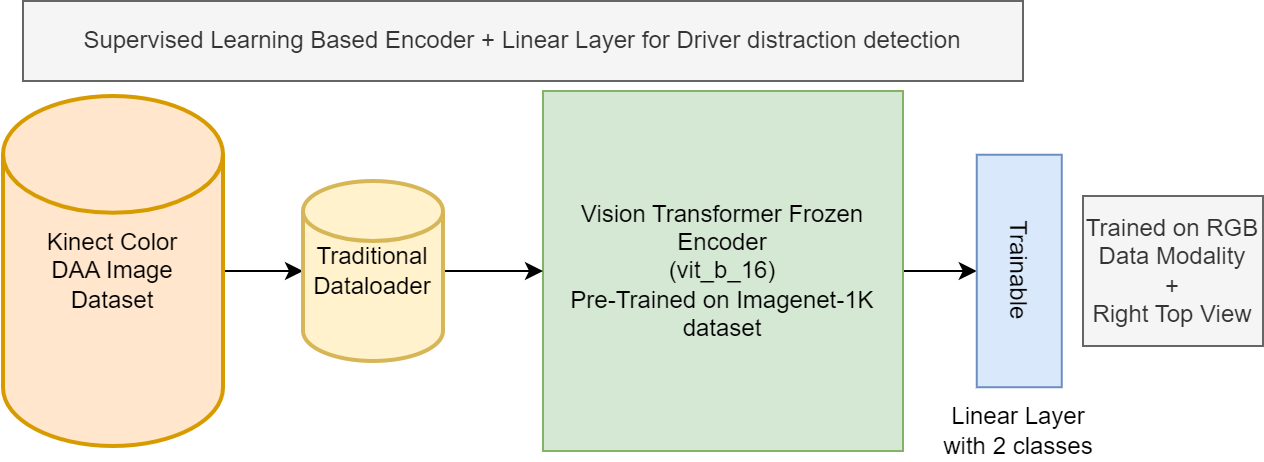
\includegraphics[width=0.8\textwidth]{Images_Thesis/methodology_images/methodology_flowchart_d_a_without_augmentation_final_2.png}
\end{center}
\caption[Methodology for supervised learning based pre-trained encoder for downstream task of driver distraction detection.]{Methodology for supervised learning based pre-trained encoder for downstream task of driver distraction detection.}
\label{fig:method_flow_chart_d_a_without_aug}
\end{figure}

\subsection{Experiment 2: Supervised Learning Based Encoder with Gray scale Augmentation}
\label{section:Methodology 2 Experiment 2: Supervised Learning Based Encoder with Gray scale Augmentation}
Figure~\ref{fig:method_flow_chart_d_a_with_aug} outlines the methodology for this experiment, which mirrors Experiment 1 with a significant variation: the addition of grayscale augmentation. This experiment was designed to explore the impact of grayscale augmentation on model generalization, particularly under low-light or night time driving conditions where color images may offer limited information. We hypothesized that grayscale images might yield better generalizability in such scenarios. Thus, we trained our hybrid classifier with grayscale augmentation for 100 epochs and subsequently evaluated its effectiveness.
\begin{figure}[h]
\begin{center}
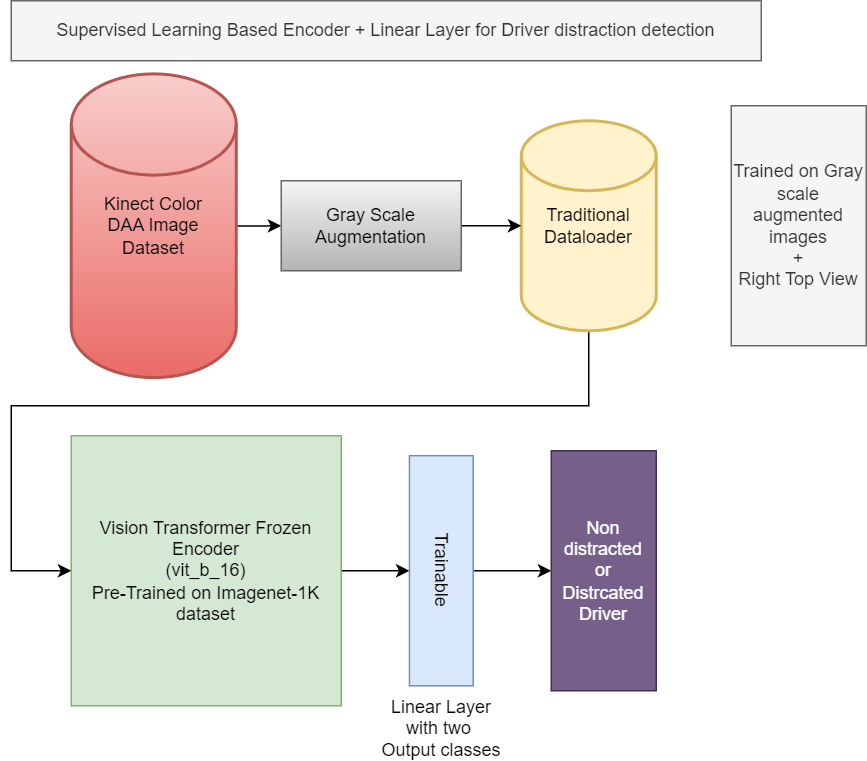
\includegraphics[width=0.8\textwidth]{Images_Thesis/methodology_images/methodology_flowchart_d_a_with_augmentation.png}
\end{center}
\caption[Methodology for supervised learning based pre-trained encoder with gray scale augmentation for downstream task of driver distraction detection.]{Methodology for supervised learning using a pre-trained encoder with grayscale augmentation for driver distraction detection. The figure shows grayscale transformations applied during data loading, incorporating IR modality knowledge to fine-tune a linear layer on a frozen encoder.}
\label{fig:method_flow_chart_d_a_with_aug}
\end{figure}

\subsection{Experiment 3: Self-Supervised Learning (SSL) Based Encoder}
\label{section:Methodology Experiment 3: Self-Supervised Learning Based Encoder}
The methodology for this experiment is depicted in figure~\ref{fig:method_flow_chart_d_a_ssl}. We utilized a vision transformer encoder, vit\_b\_14~\citep{dinov2_github}, trained with the DINOv2 SSL method on the extensive, unlabeled LVD-142M~\citep{dinov2_oquab2023dinov2} dataset. The encoder, frozen to preserve its feature-extracting capabilities, processes image batches to serve as inputs to a linear classifier designed for detecting driver distractions. This setup allowed us to train the linear layer of the model on the color modality with a right top view and evaluate its performance on unseen test datasets. This experiment aims to compare the performance of linear layer fine tuned on top of self-supervised learning-based frozen encoder against Experiments 1 and 2. For a balanced comparison, we will evaluate the 100th checkpoint of the finely-tuned linear layers across all experiments, assessing both validation and test balanced accuracy scores.

\begin{figure}[h]
\begin{center}
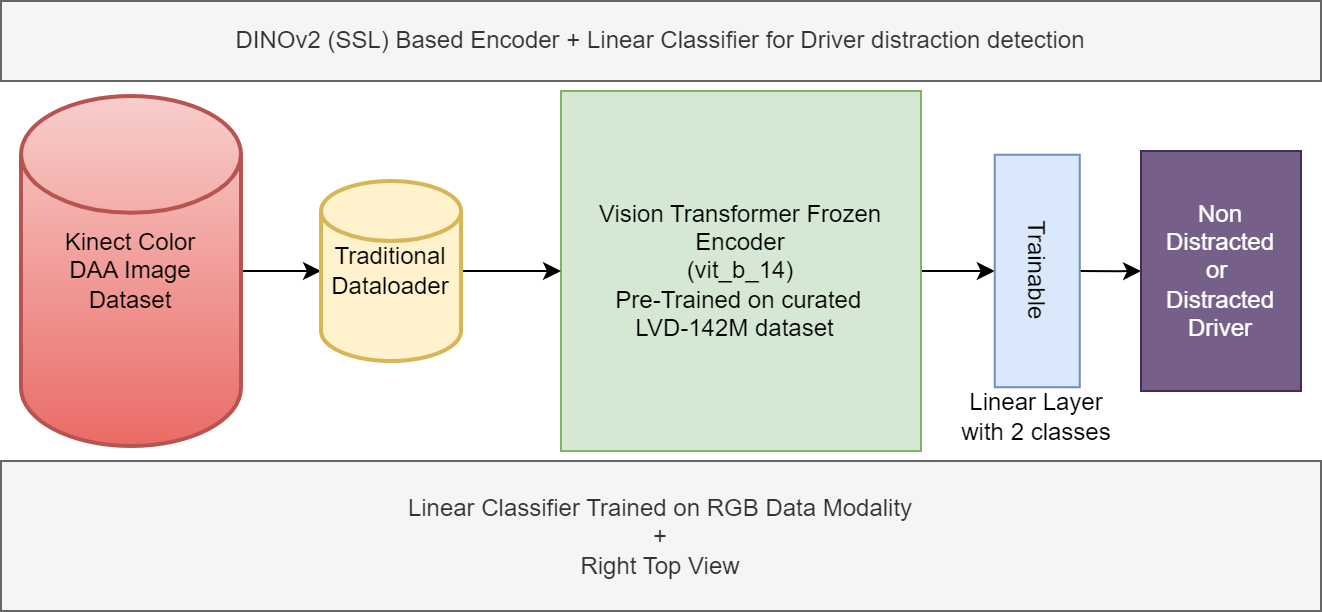
\includegraphics[width=0.8\textwidth]{Images_Thesis/methodology_images/methodology_flowchart_ssl_d_a.png}
\end{center}
\caption[Methodology for self-supervised learning based pre-trained encoder for downstream task of driver distraction detection.]{Methodology for self-supervised learning based pre-trained encoder (DINOv2 vit\_b\_14) for downstream task of driver distraction detection. The figure depicts the traditional dataloading of the Kinect Color DAA dataset and fine-tuning of a linear layer on top of frozen encoder for downstream driver distraction detection task.}
\label{fig:method_flow_chart_d_a_ssl}
\end{figure}

\subsubsection{Choice of Linear Evaluation protocol}
The authors of the~\citep{dinov2_oquab2023dinov2} have used both kNN and linear evaluation protocols in their research. But in this thesis, the DINOv2 based `vit\_b\_14' encoder~\citep{dinov2_oquab2023dinov2}, pretrained on curated LVD-142M unlabeled dataset, is tested using the linear probing on the Kinect color right top drive and act image dataset. This decision is guided by several factors:
\begin{itemize}
    \item \textbf{Computational Efficiency:} Linear evaluation requires considerably less computational resources compared to full fine-tuning and can be executed relatively quickly~\citep{ssl_codebook_balestriero2023cookbook}.
    \item \textbf{Direct Assessment of Representational Quality:} Since linear probing focuses purely on the discriminative power of the pre-trained features without allowing significant model adaptation, it provides a clear indication of the quality of the \gls{ssl}-induced features~\citep{ssl_zhang_2016_colorful, ssl_codebook_balestriero2023cookbook}.
    \item \textbf{Practical Relevance:} Training a linear classifier on a fixed backbone roughly replicates real-world scenarios, where \gls{ssl} models are often used as feature extractors in larger systems~\citep{ssl_zhang_2017split, ssl_codebook_balestriero2023cookbook}.
\end{itemize}

\subsection{Experiment 4: SSL Based Encoder with Clustered Feature Weighting}
\label{section: Methodology Experiment 4: Self-Supervised Learning Based Encoder with Clustered Feature Weighting Data-loading}
Figure~\ref{fig:method_flow_chart_d_b_ssl} details this experiment's methodology, highlighting the use of a clustered feature weighting data loading technique, a deviation from traditional data loading approaches. This method is expected to enhance model training and generalization across unseen datasets and different modalities or views. The same encoder and linear layer configuration from Experiment 3 is employed, but with the clustered feature weighting strategy during model training.
\begin{figure}[h]
\begin{center}
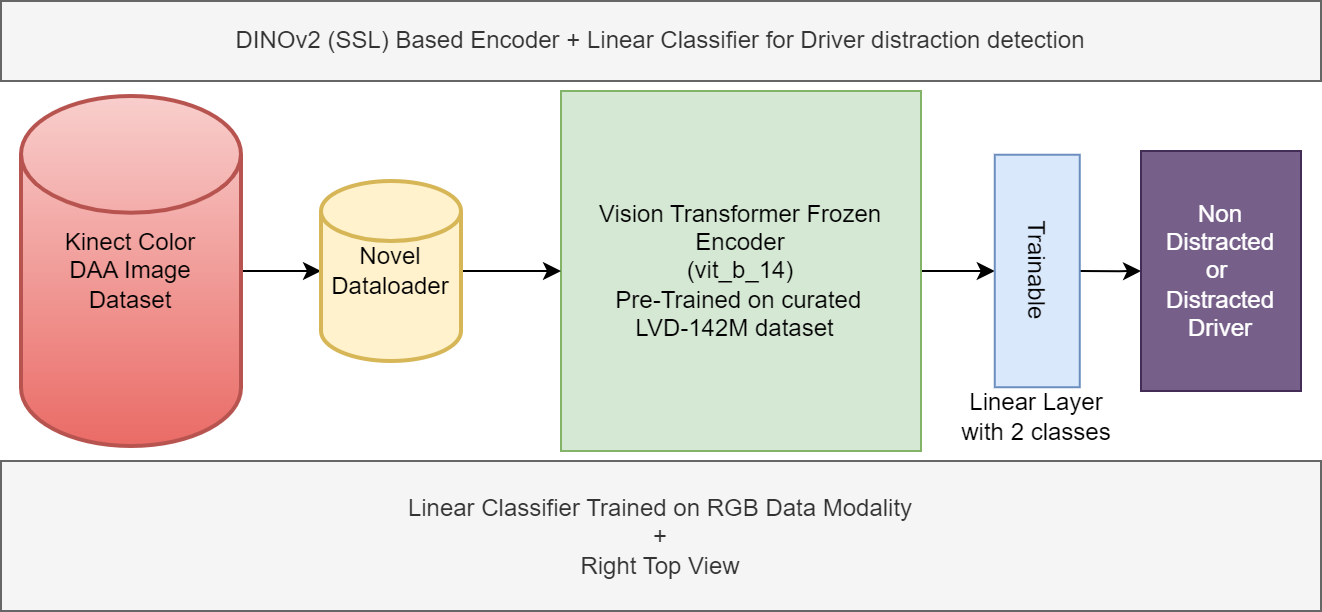
\includegraphics[width=0.8\textwidth]{Images_Thesis/methodology_images/methodology_flowchart_d_b_ssl.png}
\end{center}
\caption[Methodology for self-supervised learning based pre-trained encoder with Clustered Feature Weighting Data-loading for downstream task of driver distraction detection.]{Methodology for self-supervised learning based pre-trained encoder (DINOv2 vit\_b\_14) with Clustered Feature Weighting Data-loading for downstream task of driver distraction detection. In the figure novel dataloader corresponds to Clustered Feature Weighting based dataloader.}
\label{fig:method_flow_chart_d_b_ssl}
\end{figure}

\paragraph{Data Transformations in Experiment 3 and 4:}
Data transformation strategies are crucial for training robust models. We employed the same data transformation strategy for both training and evaluation phases as described and used in~\citep{dinov2_oquab2023dinov2} for linear probing.
\paragraph{Training Transforms:}
The training transforms includes a series of transformations to simulate diverse viewing conditions:
\begin{itemize}
    \item \textbf{RandomResizedCrop}: Applied with bicubic interpolation to preserve image quality while adjusting sizes. The crop size used is 224.
    \item \textbf{RandomHorizontalFlip}: Conditionally applied based on a 0.5 probability to introduce horizontal asymmetry.
    \item \textbf{MaybeToTensor}: Ensured all inputs were converted to tensors to accommodate different formats.
    \item \textbf{Normalization}: Used predefined ImageNet~\citep{Imagenet1k_ILSVRC15} mean and standard deviation values to standardize inputs.
\end{itemize}

\paragraph{Evaluation Transforms:}
The evaluation transforms aimed for consistency and reproducibility:
\begin{itemize}
    \item \textbf{Resize and CenterCrop}: First the image is resized to a size 256 using bicubic interpolation to ensure high-quality image representation at standard dimensions. Then the CenterCrop with crop size 224 is applied.
    \item \textbf{MaybeToTensor and Normalization}: Consistently prepared and standardized inputs, similar to training transforms.
\end{itemize}

\subsection{Methodology for Cross-Modality Generalization Evaluation}
\label{section:Methodology for Cross-Modality Generalization Evaluation}
Figure~\ref{fig:method_flow_chart_cross_modality_gen} illustrates the cross-modality generalization approach. We evaluated the 100th epoch checkpoints of the trained encoders on the KIR Right Top and NIR Front Top IR datasets, which present different imaging modalities (IR) compared to the color data used in model training. This experiment seeks to understand the adaptability of models to different sensory information, relevant in diverse lighting conditions.

\begin{figure}[h]
\begin{center}
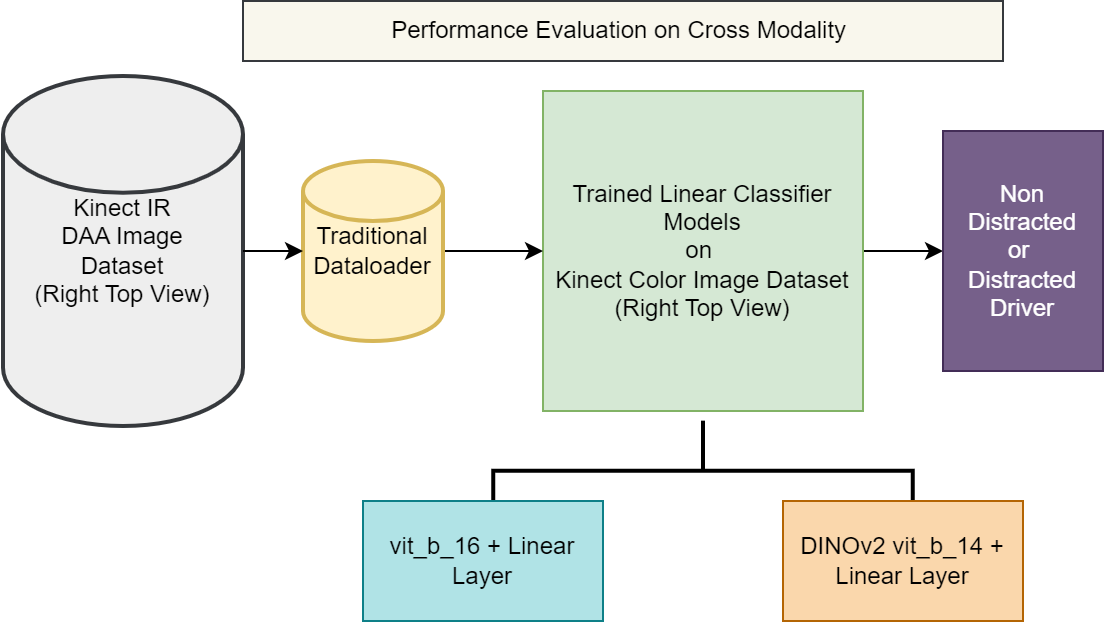
\includegraphics[width=0.8\textwidth]{Images_Thesis/methodology_images/methodology_cross_modality_generalisation.png}
\end{center}
\caption[Methodology for cross-modality generalisation.]{Methodology for cross-modality generalisation for downstream task of driver distraction detection. KIR Right Top view dataset only differs in the modality of data when compared with Kinect Color Right Top view dataset. Hence, using Kinect IR DAA test sets, the cross-modality evaluation across all four experimental scenarios is performed.}
\label{fig:method_flow_chart_cross_modality_gen}
\end{figure}

\subsection{Methodology for Cross-View Generalization Evaluation}
\label{section:Methodology for Cross-View Generalization Evaluation}
Figure~\ref{fig:method_flow_chart_cross_view_gen} shows the methodology for cross-view generalization. Here, we assess the models trained on the right view Kinect color image DAA dataset against the NIR Front Top dataset, which provides a different camera perspective. This experiment aims to verify the models' robustness to varying viewpoints, simulating real-world scenarios where camera angles can differ unexpectedly.

\begin{figure}[h]
\begin{center}
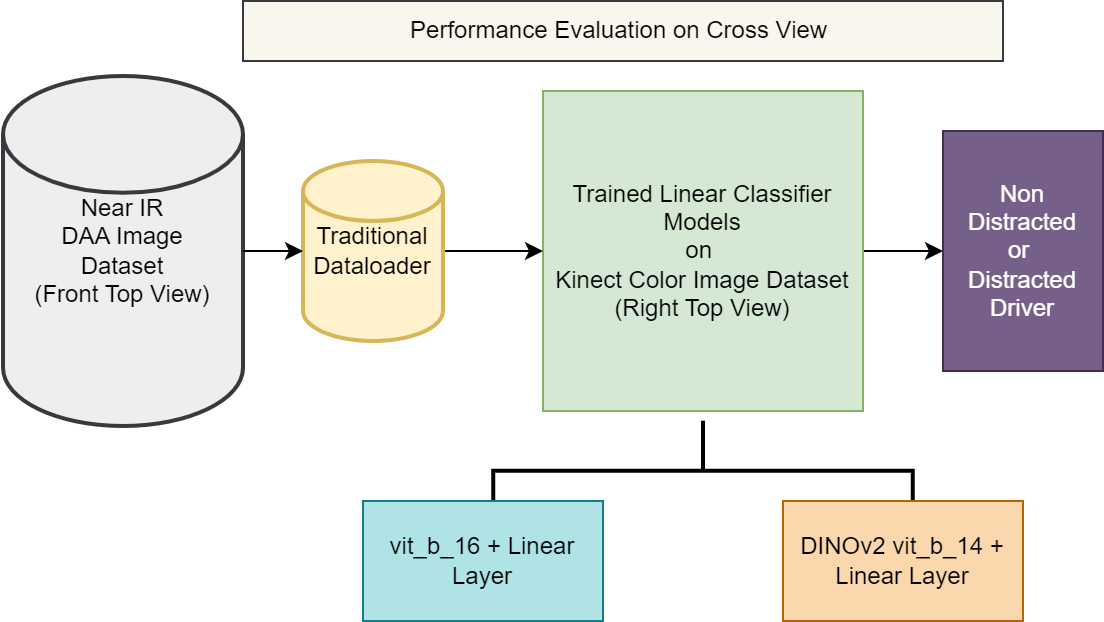
\includegraphics[width=0.8\textwidth]{Images_Thesis/methodology_images/methodology_cross_view_generalisation.png}
\end{center}
\caption[Methodology for cross-view generalisation.]{Methodology for cross-view generalisation for downstream task of driver distraction detection. In the figure, the NIR DAA dataset is used with front top view and Ir modality for cross-view and cross modality generalisation. This evaluation done in all four experiments using both types of encoder under consideration as depicted in the figure.}
\label{fig:method_flow_chart_cross_view_gen}
\end{figure}



%%%%%%%%%%%%%%%%%%%%%%%% Chapter 5: Experiments %%%%%%%%%%%%%%%%%%%%
%%%%%%%%%%%%%%%%%%%%%%%%%%%%%%%%%%%%%%%%%%%%%%%%%%%%%%%%%%%%%%%%%%%
%%%%%%%%%%%%%%%%%%%%%%%%%%%%%%%%%%%%%%%%%%%%%%%%%%%%%%%%%%%%%%%%%%%
%%%%%%%%%%%%%%%%%%%%%%%%%%%%%%%%%%%%%%%%%%%%%%%%%%%%%%%%%%%%%%%%%%%
\chapter{Experiments and Results}
\label{chapter:Experiments and Results}
In Chapter 4, we outlined the methodologies employed across various experiments integral to this thesis. Building on that foundation, Chapter 5 presents the empirical evidence validating the methods and concepts previously discussed. We begin by detailing the experimental setup, including a description of the datasets and models utilized, as well as the computational resources involved. This is followed by an analysis of experiments focused on our novel data loading technique, presenting specific results from these experiments.

Subsequent sections delve into the outcomes of Experiments 1 through 4, examining their effectiveness in cross-modality and cross-view generalization. Each experiment is contextualized with comprehensive results, facilitating a thorough understanding of their impact and significance.

This chapter aims to solidify the empirical groundwork for the conclusions drawn in the subsequent final chapter, where these results are synthesized into a cohesive conclusion regarding the thesis objectives.

\section{Experimental Setup}
\subsection{Datasets}
For our experiments we have utilized three distinct datasets derived from the DAA video dataset as listed below:
\begin{enumerate}
    \item \textbf{Kinect Color Right Top Image DAA Dataset}: Consists of RGB images used to train and evaluate the model’s ability to detect distracted and non-distracted drivers. The train dataset from split 0 of this dataset is utilized for dataloader experiments. The train and validation datasets from split 0 of this dataset are used for hyperparameter search.
    \item \textbf{Kinect IR Right Top Image DAA Dataset}: Comprises grayscale images where each channel replicates the same grayscale information, used primarily to test the models' generalization across different imaging modalities.
    \item \textbf{NIR Front Top Image DAA Dataset}: Contains grayscale images similar to the Kinect IR dataset but from a front top viewpoint. It is used to assess the models' capacity to generalize across front top view and \gls{inr} modality.
\end{enumerate}

\subsection{Model Architectures}
Three primary models are utilized in this thesis:
\begin{itemize}
    \item \textbf{Feature Extraction Model}: The `vit\_huge\_patch14\_224.orig\_in21k'~\citep{huggingface_vit} model is used for feature extraction in the~\ref{section:dataloader experiments}, where the novel `Clustered Feature Weighting' data loading startegy is evaluated. The model is accessed from Huggingface librray. Equipped with 658.7 million parameters and pretrained on the ImageNet-21K dataset, this model efficiently extracts features from image datasets. It expacts an input image of size 224 x 224 pixels and extract a [1 x 1280] feature vector for a batch of single image.
    \item \textbf{Supervised Learning based pre-trained Vision Transformer}: The `vit\_b\_16'~\citep{vit_b_16_pytorch} model accessed from the Torchvision library, pretrained on imagenet-1K dataset is used as a supervised encoder. It served as a pretrained backbone, on top of which a zero initialized linear layer with two output classes is used to classify `non distracted' and `distracted' driver classes in experiment 1 and 2. Total parameters in the resulted model are 85,800,194 out of which total trainable parameters are 1538.
    \item \textbf{Self-Supervised learning based pre-trained Vision Transformer (vit\_b\_14)}: The DINOv2 `vit\_b\_14'~\citep{dinov2_github} model is accessed from Pytorch hub, it is pretrained on the unlabeled curated LVD-142M dataset via the DINOv2~\citep{dinov2_oquab2023dinov2} self-supervised learning approach. It served as a backbone in experiments 3 and 4. A linear classifier is defined with frozen backbone to utilize the pre-trained weights of the `vit\_b\_14' encoder on the driver distraction detection task. The linear layer is initialised with weights drawn from a normal distribution with (mean = 0 and standard deviation = 0.01) and bias = 0. Total parameters in the resulted model are 86,582,018 out of which total trainable parameters are 1538.
\end{itemize}

\subsection{Computational Resources}
The experiments from 1 to 3 utilized dual NVIDIA Tesla V-100-SXM2-32 GB GPUs setup. Most training was facilitated via the Distributed Data Parallel (DDP)~\citep{DDP_pytorch_DBLP:journals/corr/abs-2006-15704, pytorch_ddp} algorithm to enhance computational efficiency across two GPUs. The effective batch size used is 1024 which means a batch size of 512 per gpu in DDP setup. The experiment 4, using `ClusteredFeatureWeighting' data loading strategy, utilized a single GPU with the same effective batch size for fair comparison.

\section{Results of Dataloader Experiments}
\label{section:dataloader experiments}
The novel data loader proposed in this thesis promotes a fairer evaluation of model performance across different classes by ensuring a more equitable class representation in each training batch. It also aims at improving the trained models' overall robustness and reliability.

\subsection{Assessment of the Vision Transformer Model as a Feature Extractor}
This section details the performance of the Vision Transformer model `vit\_huge\_patch14\_224.orig\_in21k`~\citep{huggingface_vit} in extracting features. Equipped with 658.7 million parameters and pretrained on the ImageNet-21K~\citep{Imagenet_21K_ridnik2021imagenet} dataset, this model efficiently extracts features from the Kinect Color Right Top Image dataset. We resize each image to 224 x 224 pixels and extract a [1 x 1280] feature vector, culminating in a [1024 x 1280] embedding for batches of 1024 images.

The primary aim of this experiment was to evaluate the variance of features within and across classes after extraction. We organized features by class from the Kinect Color DAA's training dataset (split 0). The feature dimensions for the `non-distracted' class were [79934 x 1280], and for the `distracted' class were [179931x1280]. We calculated intra-class variance vectors for each class (Equations~\ref{equation:4.8}), determined class centers (Equations~\ref{equation:4.9} and \ref{equation:4.10}), assessed inter-class variance (Equation~\ref{equation:4.11}), and measured the distance between class centers (Equation~\ref{equation:4.12}), which was found to be 0.366.

Figure~\ref{fig:variance_analysis_image} presents the variance spread across the 1280 dimensions, normalized to the maximum variance value observed. This normalization facilitates direct comparison across variances, aiding in identifying the most variable and potentially discriminative features. The analysis is crucial for understanding how effectively the feature extractor can differentiate between `distracted' and `non-distracted' categories.

\paragraph{Intra-Class Variance:} The visualization indicates that Class 0 (blue) generally displays lower variance, suggesting more homogeneity within this class compared to Class 1 (red), which shows higher variance due to its larger sample size and greater diversity.

\paragraph{Inter-Class Variance:} Represented by a green line, the inter-class variance indicates that the average features of the two classes are similar across many dimensions, highlighting the need for a more effective feature extraction approach to enhance class distinction.

Notably, the higher intra-class variances (peaks in red and blue lines) pinpoint dimensions where data points are more dispersed, providing insights into class characteristics. Features showing higher inter-class variance are critical for distinguishing between classes. Our analysis indicates moderate separability, suggesting that more sophisticated models or feature transformations may be necessary to improve class distinction. However, the existing feature distinction suffices for evaluating the novel dataloader approach.

\begin{figure}[htbp]
\begin{center}
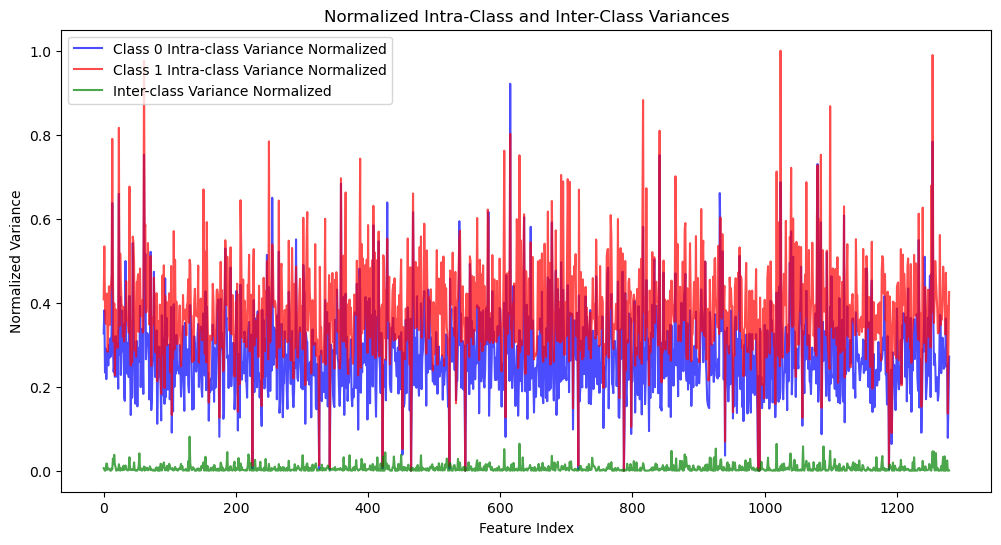
\includegraphics[width=0.8\textwidth]{Images_Thesis/variance_d_b/output_normalized_variance_07.png}
\end{center}
\caption[Feature variance analysis using the vision transformer model.]{Feature variance analysis using the vision transformer model. Displays intra-class variance curves for `non-distracted' (blue) and `distracted' (red) drivers, with the green line depicting inter-class variance. The x-axis denotes the 1280 features extracted, and the y-axis shows normalized variance values, using the highest observed variance of 0.00423 for normalization.}
\label{fig:variance_analysis_image}
\end{figure}

\paragraph{Challenges in Class Separability:}
The analysis indicates a low inter-class variance of approximately 0.01 and a distance of 0.366 between class centers, suggesting the model's limitations in distinct class differentiation. Nonetheless, these limitations are less critical as the model's primary function is to enrich the input for clustering and weighting rather than direct classification. The HDBSCAN algorithm leverages the broad spectrum of extracted features to generate meaningful clusters, which are more valuable than outright class separability for this application.

This strategy enhances training batch diversity, crucial for improving generalization in the subsequent model training. A weighting strategy that assigns lower weights to outliers (0.001) ensures that these atypical features do not disproportionately influence the training process, mitigating potential biases from high intra-class variance.

Overall, while the feature extraction model may not excel in class discrimination, it captures an extensive range of class features essential for effective clustering and weighted sampling, thus addressing challenges in training with imbalanced and complex datasets.

\subsection{Dataloader Comparison}
In addressing the first research question concerning the issue of data imbalance in the DAA dataset, this section evaluates whether unsupervised learning techniques can effectively rectify this imbalance. Previous studies, as outlined in the chapter~\ref{chapter:related_work}, provide various methods to tackle dataset imbalances, each with distinct advantages and limitations. This thesis proposes an unsupervised learning-based data loading strategy termed ``Clustered Feature Weighting,'' aiming to enhance batch balance during data loading for training deep learning models.

\paragraph{Experiment Setup:}
To assess the efficacy of the ``Clustered Feature Weighting'' strategy against traditional data loading methods, where training data is loaded without addressing imbalances, an experimental comparison was conducted. Detailed methodologies are presented in the methodology section; here, we focus exclusively on the experimental results.

\paragraph{Settings for Clustering \& Weighting:}
\begin{itemize}
    \item \textbf{Algorithm}: HDBSCAN
    \item \textbf{Metric}: Batchwise Cosine Distance Matrix
    \item \textbf{Minimum Cluster Size}: 25
    \item \textbf{Minimum Samples (min\_samples)}: 1
    \item \textbf{Cluster Selection Epsilon}: 0
    \item \textbf{Metric Type}: Precomputed
    \item \textbf{Cluster Selection Method}: EOM
    \item \textbf{Allow Single Cluster}: No
    \item \textbf{Sample Weighting}: $\frac{1}{\text{Number of samples in the cluster}}$
    \item \textbf{Outlier Weight}: 0.001
\end{itemize}

\paragraph{Results:}
Figure~\ref{fig:kl_divergence_plot_0_001} illustrates the KL divergence for dataloader comparison. This plot compares the KL divergence between the ideal uniform distribution per batch per category (shown in red) and the distributions achieved by Traditional Dataloader A (blue) and Clustered Feature Weighting Dataloader B (orange). The y-axis represents the KL divergence value, while the x-axis shows the number of batches with a batch size of 1024 for the split 0 train dataset of Kinect Color Right Top Image DAA, containing 259,865 total image samples. A lower KL divergence value indicates a closer approximation to the ideal uniform distribution.

\begin{figure}[h]
\begin{center}
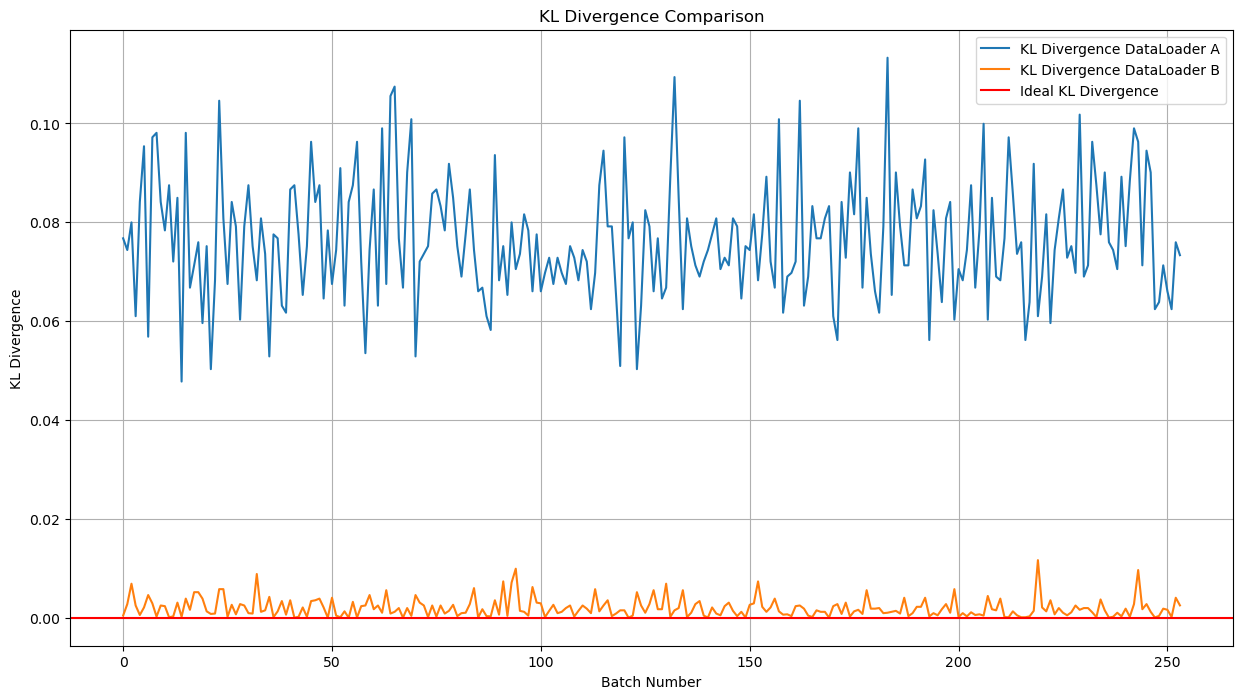
\includegraphics[width=0.8\textwidth]{Images_Thesis/Dataloader_comp/Images_0_001/output_with_uniform_kl_results_grid_0_001.png}
\end{center}
\caption[Comparative KL divergence analysis across multiple batches for dataloading strategies.]{Comparative KL Divergence Analysis Across Multiple Batches for Two Dataloading Strategies. This plot visualizes the KL divergence values on the y-axis against the batch numbers on the x-axis, comparing the uniformity of category distribution per batch between the traditional dataloading approach (Dataloader A, shown in blue) and the novel clustered feature weighting strategy (Dataloader B, shown in orange). The plot demonstrates how closely each strategy approximates the ideal uniform distribution across categories, highlighting the effectiveness of the clustered feature weighting in achieving more balanced data loading.}
\label{fig:kl_divergence_plot_0_001}
\end{figure}

\paragraph{Analysis of KL Divergence Plot:}
\begin{itemize}
    \item \textbf{General Trend}: Both lines on the plot denote the KL divergence for each batch, with Dataloader A depicted in blue and Dataloader B in orange.
    \item \textbf{Dataloader A (Blue Line)}: The values fluctuate around 0.08 and higher, suggesting significant divergence from the uniform distribution. This indicates imbalanced class representation within each batch, particularly with over-representation of the `distracted' driver category.
    \item \textbf{Dataloader B (Orange Line)}: The values generally remain below 0.01, close to the ideal zero, which indicates a more balanced class representation within batches.
\end{itemize}

\paragraph{Interpretation and Assessment:}
\begin{itemize}
    \item \textbf{Balanced Sampling}: Dataloader B's performance, characterized by lower and more stable KL divergence values, demonstrates its effective balanced sampling across categories. This contrasts with Dataloader A, which shows greater batch-to-batch category imbalance.
    \item \textbf{Consistency and Predictability}: Dataloader B exhibits consistent and predictable sampling behavior, essential for stable deep learning training. In contrast, the imbalance observed in Dataloader A could potentially lead to less effective model training and generalization.
    \item \textbf{Suitability for Deep Learning Experiments}: Given the goal of achieving a balanced and unbiased representation of categories in training batches, Dataloader B is preferable for training robust deep learning models. It potentially reduces the risk of overfitting to dominant categories.
\end{itemize}

\begin{figure}[htbp]
    \centering
    % First row
    \begin{subfigure}[b]{0.7\textwidth}
        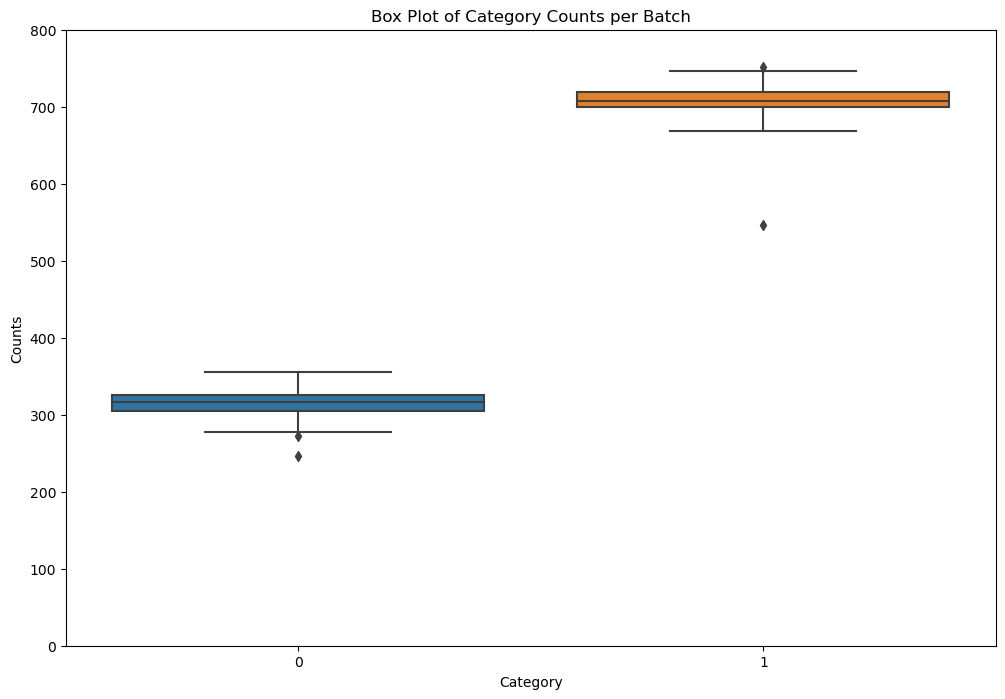
\includegraphics[width=\textwidth]{Images_Thesis/Dataloader_comp/Images_0_001/output_d_a_binary_box_plot_0_001.png}
        \caption{Dataloader A-Traditional Dataloading without Balancing.}
        \label{fig:Box plot for 0_001 experiment with dataloader A}
    \end{subfigure}
    \hfill % space between images
    \begin{subfigure}[b]{0.7\textwidth}
        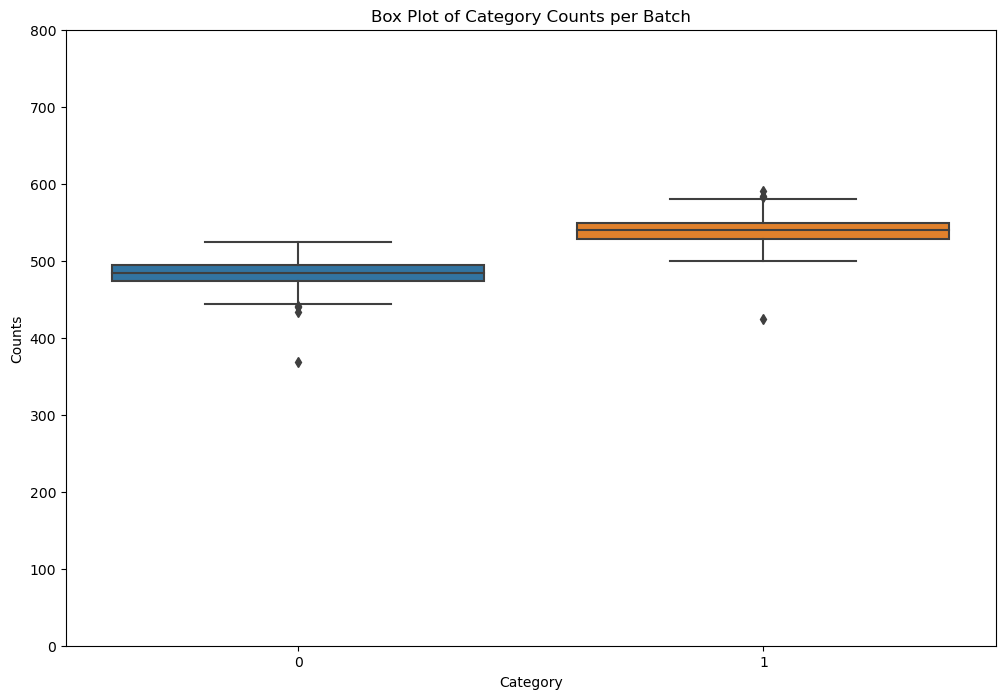
\includegraphics[width=\textwidth]{Images_Thesis/Dataloader_comp/Images_0_001/output_d_b_box_plot_0_001.png}
        \caption{Dataloader B-With Clustered Feature Weighting Strategy for Balancing.}
        \label{fig:Box plot for 0_001 experiment with dataloader B (novel)}
    \end{subfigure}

    \caption[Box plot analysis of sample counts per batch for dataloading strategies.]{Box Plot Analysis of Sample Counts per Batch for Two Dataloading Strategies. This figure displays box plots that illustrate the distribution of sample counts per batch for nondistracted (Category 0) and distracted (Category 1) driver categories, using both (a) Dataloader A and (b) Dataloader B. The box plots show the spread, central tendency, and outliers for each category within the batches. Dataloader B, which employed an outlier weight of 0.001, demonstrates how this parameter influences the balance and uniformity of sample distribution compared to Dataloader A.}
    \label{fig:Box plot dataloader A and dataloader B with 0_001}
\end{figure}

%%%%%%%%%%%%%%%%%% Grid of class distributions %%%%%%%%%%%%%%%%%
\paragraph{Analysis of Category Counts per Batch Using Box Plots:}
Figure~\ref{fig:Box plot dataloader A and dataloader B with 0_001} presents a box plot visualization of the counts of samples per batch for two categories of driver distraction: nondistracted (Category 0) and distracted (Category 1) across two different dataloaders under comparison, A and B. These box plots are instrumental in assessing the balance of sample distribution across categories within each batch.

In Dataloader A, see~\ref{fig:Box plot dataloader A and dataloader B with 0_001}-(a), the median count for Category 0 (non-distracted) is notably lower at approximately 310 counts, whereas for Category 1 (distracted), it is significantly higher at about 710 counts. This discrepancy indicates a skewed distribution in each batch, which could lead to biased model training due to the over-representation of distracted drivers.

Conversely, Dataloader B, see~\ref{fig:Box plot dataloader A and dataloader B with 0_001}-(b), shows a more balanced approach, with the median counts for Category 0 and Category 1 being much closer to each other, around 480 and 530 counts, respectively. These values suggest a more equitable distribution of categories within batches, which is closer to the ideal scenario where each category would ideally comprise half of the batch size of 1024, meaning 512 samples from Category 0 and 512 samples from Category 1. The comparison of these medians between the two dataloaders indicates that Dataloader B is more effective in creating balanced batches.

\paragraph{Impact of Outlier Weight on Sampling:}
The selection of an outlier weight of 0.001 in our experiments was a deliberate decision informed by extensive empirical testing. This parameter was fine-tuned through a systematic trial-and-error process, exploring a range of values from 0 to 1. The impact of the outlier weight on the sampling process is crucial, as it directly influences the KL divergence values, which measure the discrepancy between the actual data distribution in each batch and the ideal uniform distribution across categories.

Figure~\ref{fig:kl_divergence_plot_0_02} illustrates the effects of utilizing a higher outlier weight of 0.02 in Dataloader B. The results indicate a significant increase in the KL divergence values, averaging around 0.07, which suggests a deviation from the ideal uniform distribution. This deviation is substantiated by the increased KL divergence, highlighting the sensitivity of the sampling process to the outlier weight setting.

Moreover, the corresponding box plots in Figure~\ref{fig:Box plot for 0_02 experiment with dataloader B (novel)} for categories 0 and 1 reveal a noticeable difference between the medians of counts of each category. This difference underscores a pronounced imbalance in the batch compositions of Dataloader B when a higher outlier weight is employed. The divergence of the medians from each other at this higher outlier weight (0.2) confirms that the distribution of samples across categories becomes significantly skewed, detracting from the efficacy of the dataloading process in maintaining balanced batches.

\begin{figure}[htbp]
\begin{center}
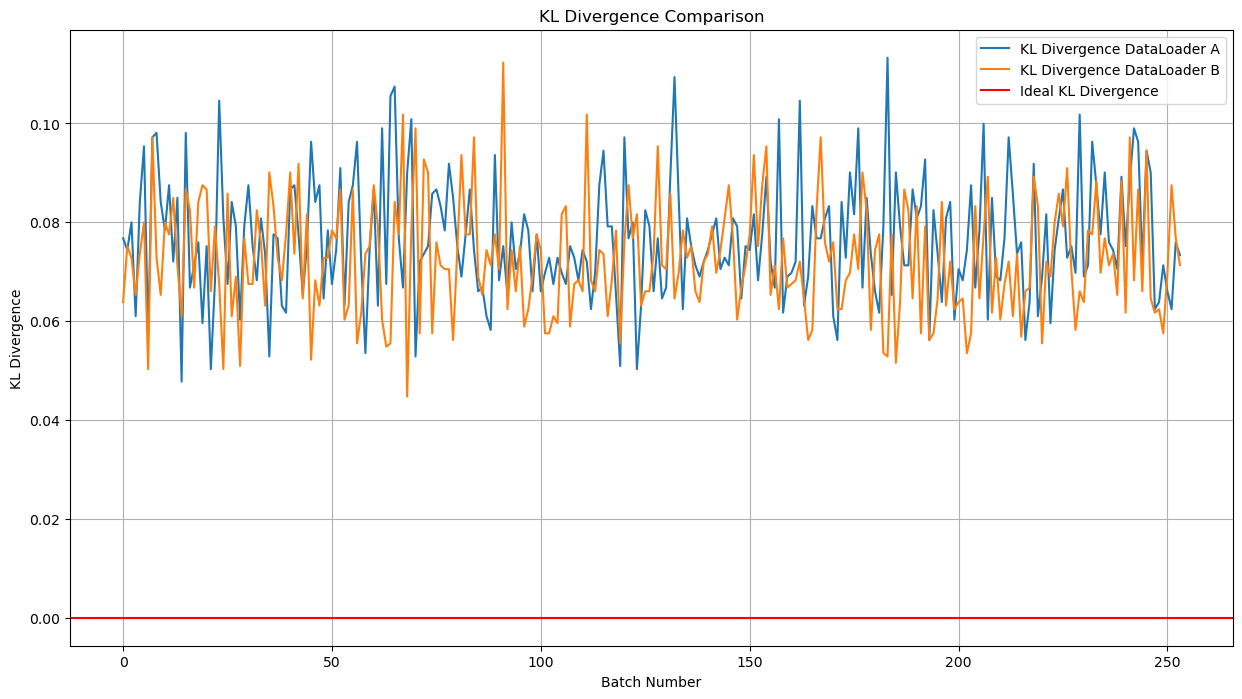
\includegraphics[width=0.8\textwidth]{Images_Thesis/Dataloader_comp/Images_0_02/output_0_02_outlier_weight_KL.png}
\end{center}
\caption[KL divergence analysis with increased outlier weight.]{KL Divergence Analysis with Increased Outlier Weight. This plot displays the KL divergence values on the y-axis versus the number of batches on the x-axis, comparing the traditional dataloading approach (Dataloader A) and the novel clustered feature weighting strategy (Dataloader B), evaluated with an outlier weight of 0.02. The divergence from the ideal uniform distribution across categories per batch is indicated, with Dataloader B (shown in orange) and Dataloader A (shown in blue), highlighting how the increased outlier weight affects the effectiveness of each dataloading strategy in achieving category balance.}
\label{fig:kl_divergence_plot_0_02}
\end{figure}

%%%%%%%%%%%%%%%%%% Grid of class distributions %%%%%%%%%%%%%%%%%
\begin{figure}[htbp]
    \centering
    % First row
    \begin{subfigure}[b]{0.7\textwidth}
        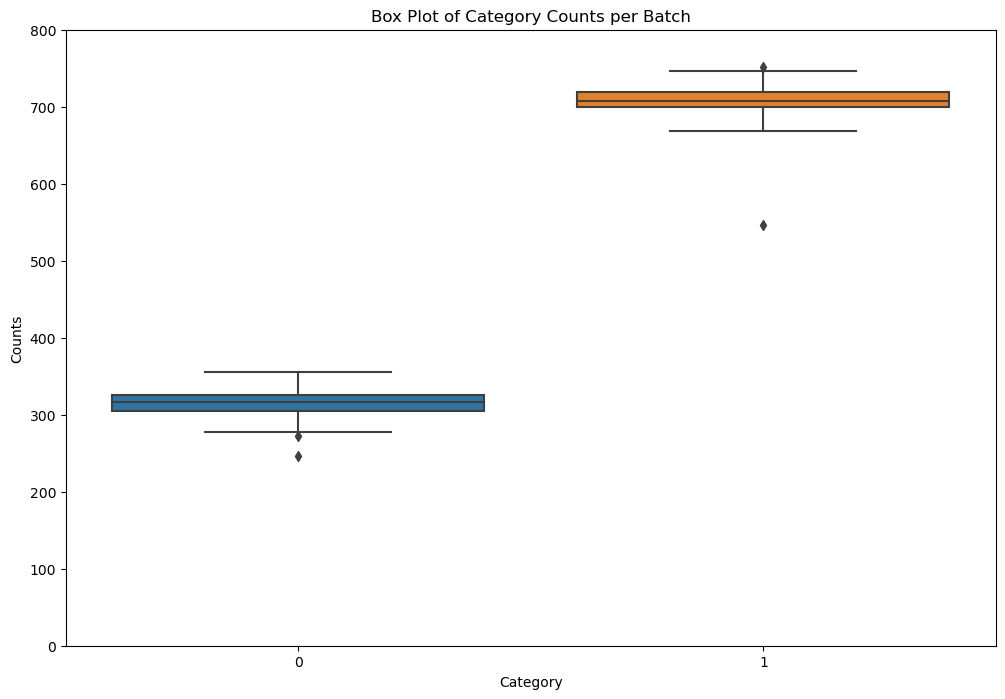
\includegraphics[width=\textwidth]{Images_Thesis/Dataloader_comp/Images_0_02/output_box_0_02_d_a.png}
        \caption{Dataloader A- Traditional Dataloading without Balancing.}
        \label{fig:Box plot for 0_02 experiment with dataloader A}
    \end{subfigure}
    \hfill % space between images
    \begin{subfigure}[b]{0.7\textwidth}
        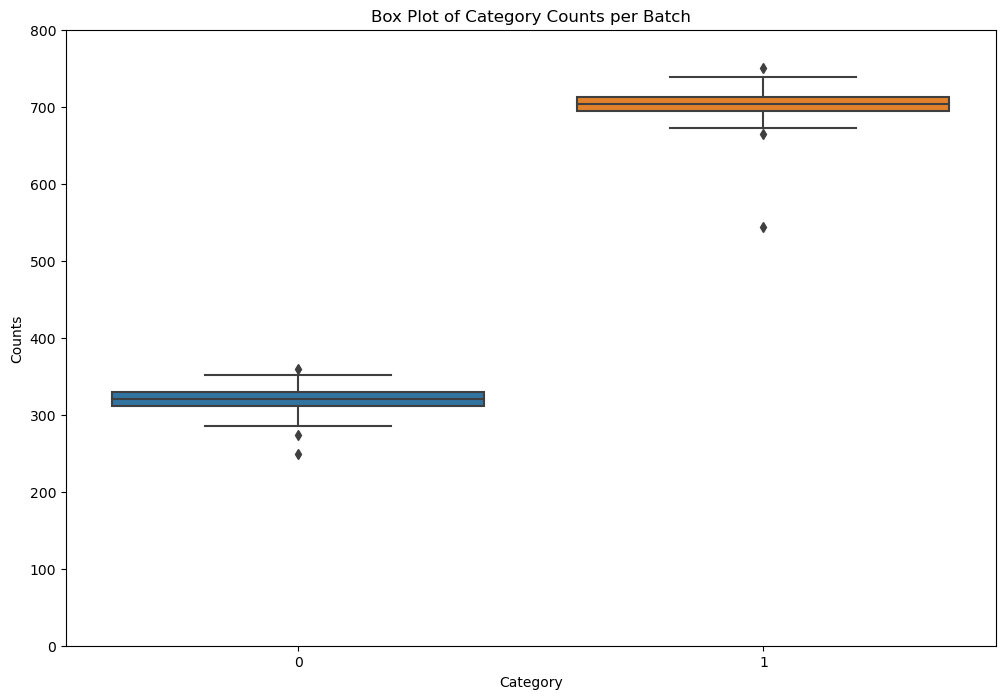
\includegraphics[width=\textwidth]{Images_Thesis/Dataloader_comp/Images_0_02/output_KL_0_02_d_b.png}
        \caption{Dataloader B- With Clustered Feature Weighting Strategy for Balancing.}
        \label{fig:Box plot for 0_02 experiment with dataloader B (novel)}
    \end{subfigure}

    \caption[Box Plot Analysis of Category Counts per Batch with an Increased Outlier Weight for Dataloader B.]{ Box Plot Analysis of Category Counts per Batch with an Increased Outlier Weight for Dataloader B. This figure presents box plots depicting the distribution of sample counts per batch for nondistracted (Category 0) and distracted (Category 1) driver categories, utilizing both Dataloader A and Dataloader B. These plots illustrate the spread, central tendency, and identification of outliers within each category's distribution across batches. Notably, Dataloader B is evaluated using an increased outlier weight of 0.02, highlighting the impact of this weight adjustment on the balance and uniformity of sample distribution compared to Dataloader A.}
    \label{fig:Box plot dataloader A and dataloader B with 0_02}
\end{figure}

\paragraph{Dataloader Experiments Conclusion:}
The comprehensive evaluation of dataloaders in this study highlights the superior performance of Dataloader B, which utilizes a clustered feature weighting strategy proposed in this thesis. This strategy significantly improves the data imbalance in training deep learning models, as demonstrated by the KL divergence and box plot analyses.

Dataloader B consistently achieved lower KL divergence values, indicating a more uniform distribution that aligns closely with the ideal uniform distribution across categories per batch. Additionally, the box plot analysis~\ref{fig:Box plot dataloader A and dataloader B with 0_001} confirmed that Dataloader B provides a more balanced distribution of both `non-distracted' and `distracted' categories within each batch. The median counts of these categories are nearly even, closely approaching the ideal split of the batch size.

In conclusion, Dataloader B ensures a more equitable representation of categories. However, this proposed novel data loading strategy still needs a verification for gain in model learning and generalisation compared to traditional dataloading.

\section{Experiments based on Model Training and Evaluation}
\subsection{Hyperparameter Grid Search Results}
A rigorous hyperparameter search was conducted using a 10\% subset of the split 0 of Kinect Color Image DAA dataset, sampled through stratified sampling method to reflect the inherent imbalance of the split 0 of the Kinect Color image DAA dataset. This process aimed to optimize model performance by identifying the most effective hyperparameters for this specific context.~\citet{Vit_Paper_Dosovitskiy2020AnII} recommended the Stochastic Gradient Descent (SGD)~\citep{pytorch_sgd} optimizer for transfer learning on vision transformer models due to its suitability in handling pretrained architectures.

The primary objective of the hyperparameter grid search was to ascertain the optimal learning rate and validate the superiority of SGD over Adam~\citep{Adam_Kingma2014AdamAM} for fine-tuning linear layer on top of frozen pre-trained vision transformers on the Kinect Color Right Top DAA dataset. Key elements of the initial setup included:
\begin{itemize}
    \item \textbf{Learning Rate Sweep:} A systematic exploration of learning rates—0.003, 0.01, 0.03, 0.06—is conducted to determine the optimal rate for training the linear layer atop the frozen encoder, gauged over 20,000 steps using validation set performance.
    \item \textbf{Steps and Epochs Calculation:} Given the 259,865 images in the train dataset of split 0 of the Kinect Color DAA Image dataset and a batch size of 1024, it takes 254 steps to complete one epoch. To achieve 20,000 steps, approximately 79 epochs are necessary. Consequently, all experiments are extended to 100 epochs to ensure adequate model convergence.
    \item \textbf{Additional Parameters:} The search also included fine-tuning parameters such as a momentum of 0.9, no weight decay, and gradient clipping at a global norm of 1 as used in the~\citep{Vit_Paper_Dosovitskiy2020AnII} for fine tuning. The resolution for fine-tuning was set at 224 pixels.
\end{itemize}

To ensure stable training conditions, the hyperparameter search was expanded to include various learning rate schedulers like Linear Decay, Step Decay, Exponential Decay, and Constant LR, alongside necessary adjustments for each strategy. Appendix section provides more details about the results of these experiments.

Experiment results, as shown in Table \ref{table:top-competitors}, indicate that training balanced accuracies are consistently high (greater than 92\%), whereas validation balanced accuracies are considerably lower (83.45\% to 83.87\%), suggesting a potential overfitting issue. Notably, the learning rate adjustments between experiments varied, with Experiment 22 starting at $4.00 \times 10^{-4}$ and reducing to $2.00 \times 10^{-4}$, and Experiment 23 implementing a higher initial rate that decreased more significantly to $1.00 \times 10^{-4}$. These configurations resulted in the smallest gaps between training and validation accuracies (8.18\% and 8.17\%, respectively), indicating better generalization compared to Experiment 25, which had a larger gap of 9.18\%. These findings underscore the importance of finely tuned learning rate schedules in balancing between achieving high training accuracy and ensuring good generalization to unseen data.

Using the Adam optimizer with cosine annealing significantly lowered performance in terms of validation accuracy; however, utilizing Adam with a linear decay scheduler, as depicted in Experiment 24 in appendix section in Table ~\ref{table:lineadecay-detailed}, yielded a validation balanced accuracy of 80.86\%, with a pronounced discrepancy of 15.80\% between training and validation accuracies. In total, 16 experiments combining the Adam and SGD optimizers with the Cosine Annealing scheduler were conducted. The maximum number of iterations (\(T_{\text{max}}\)) set for the cosine annealing was 100 and 10, as shown in the appendix section in Table~\ref{table:cosineannealing-tmax}. These experiments consistently resulted in a balanced accuracy gap exceeding 10\%, indicative of substantial overfitting. Based on the hyperparameter settings and experiments conducting using Adam and SGD optimizer, SGD optimizer performed better than Adam optimizer which aligns with the choice of~\citep{Vit_Paper_Dosovitskiy2020AnII} for fine tuning vision transformer on downstream tasks like image classification on custom datasets.

Further analysis involving the SGD optimizer paired with a Linear Decay scheduler and varying initial and final learning rates, detailed in appendix section in Table~\ref{table:lineadecay-detailed}, revealed that configurations with lower starting and ending rates effectively decreased the overfitting issue. Similarly, using the Step Decay scheduler with a decay factor of 0.1 every 20 epochs also led to overfitting, with a gap exceeding 10\%. This pattern persisted in four experiments utilizing an Exponential Decay scheduler with the SGD optimizer, refer to appendix section in Table~\ref{table:exponentialdecay-performance}, each also exhibiting significant overfitting. To assess the impact of a constant learning rate on overfitting, two additional experiments were conducted with learning rates of 0.001 and 0.003, refer to appendix section in Table ~\ref{table:constantlr-performance}, resulting in gaps of 13.70\% and 14.64\%, respectively, and validation accuracies of 81.07\% and 81.39\%.

Considering these outcomes, the hyperparameter settings from Experiment 22, which demonstrated a smaller gap between training and validation balanced accuracies, are adopted as the baseline for main experiments, as illustrated in the table~\ref{table:chosen hyperparameter configurations}.

\begin{table}[ht]
\caption{Chosen hyperparameter configurations}
\label{table:chosen hyperparameter configurations}
\centering
\begin{tabular}{ll}
\multicolumn{1}{c}{\textbf{PARAMETER}} & \multicolumn{1}{c}{\textbf{VALUE}} \\
\hline
Experiment Number & 22 \\
Epochs & 100 \\
Effective Batch Size & 1024 \\
Number of GPUs & 2 \\
Batch Size per GPU & 512 \\
Optimizer & SGD \\
Scheduler & LinearDecay \\
Initial LR & $4.00 \times 10^{-4}$ \\
End LR & $2.00 \times 10^{-4}$ \\
Train Balanced Accuracy & 92.05\% \\
Validation Balanced Accuracy & 83.87\% \\
Balanced Accuracy Gap & 8.18\% \\
\hline
\end{tabular}
\end{table}

\begin{table}[ht]
\caption{Top competing hyperparameter configurations}
\label{table:top-competitors}
\centering
\small
\begin{tabular}{llllll}
\multicolumn{2}{c}{\textbf{Experiment Details}} & \multicolumn{1}{c}{\textbf{Learning Rate}} & \multicolumn{3}{c}{\textbf{Balanced Accuracy}} \\
\hline
\textbf{Exp No} & \textbf{Optimizer-Scheduler} & \textbf{Initial LR - End LR} & \textbf{Train} & \textbf{Validation} & \textbf{Gap} \\
\hline
22 & SGD - LinearDecay & $4.00 \times 10^{-4} - 2.00 \times 10^{-4}$ & 92.05\% & 83.87\% & 8.18\% \\
23 & SGD - LinearDecay & $5.00 \times 10^{-4} - 1.00 \times 10^{-4}$ & 92.00\% & 83.83\% & 8.17\% \\
25 & SGD - LinearDecay & $4.50 \times 10^{-4} - 1.50 \times 10^{-4}$ & 92.62\% & 83.45\% & 9.18\% \\
\hline
\end{tabular}
\end{table}

\begin{figure}[htbp]
\begin{center}
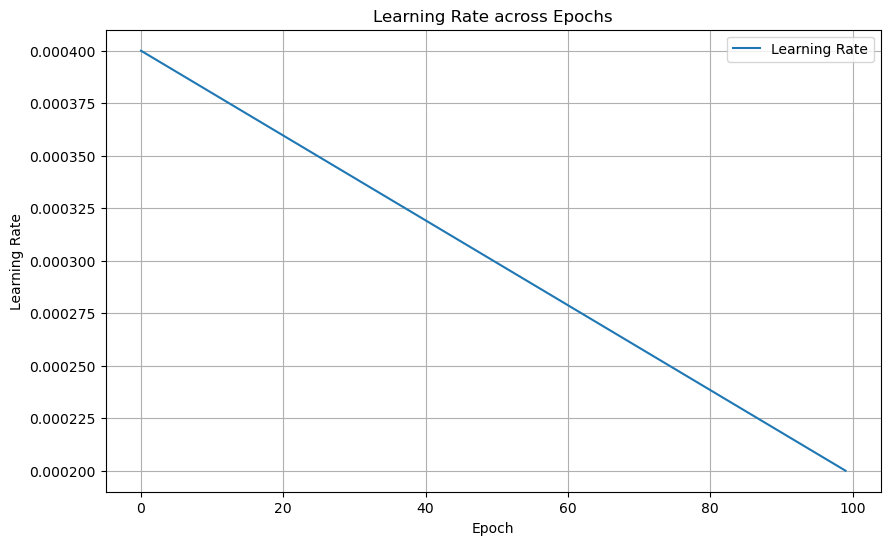
\includegraphics[width=0.8\textwidth]{Images_Thesis/Tensboard_runs_images_all/Experiment_00_Sup_D_A_no_Aug/Split_0/output_learningrate.png}
\end{center}
\caption[Linear learning rate decay used in all four experiments.]{Linear learning rate decay: the learning rate schedule starts at initial learning rate of 0.0004 and ends at 0.0002 after 100 epochs. The epochs on the x-axis are 0 indexed.}
\label{fig:learning rate plot}
\end{figure}

%%%%%%%%%%%%%%%%%%%%%%%%%%%%%%%%%%%%%%%%%%%%%%%%%%%%%%%%%%%%%%
%%%%%%%%%%%%%%%%%%%%%%%%%%%%%%%%%%%%%%%%%%%%%%%%%%%%%%%%%%%%%%
%%%%%%%%%%%%%%%%%%%%%%%%%%%%%%%%%%%%%%%%%%%%%%%%%%%%%%%%%%%%%%
\subsection{Results of Experiment 1: Supervised Learning Based Encoder}
%%%%%%%%%%%%%%%%%%%%%%%%%%%%%%%%%%%%%%%%%%%%%%%%%%%%%%%%%%%%%%
Following the methodology explained in section~\ref{section:Methodology Experiment 1: Supervised Learning Based Encoder}, in this experiment, we adapted a pre-trained Vision Transformer (vit\_b\_16) model, pre-trained on the ImageNet-1K dataset, for the driver distraction detection task using the Kinect Color Right Top view dataset. We replaced the (vit\_b\_16) classifier layer with a linear layer, training only this component to leverage the model's transfer learning and feature extraction capabilities. The hyperparameters selected in the previous section played a crucial role in training our model. These included a linear decay scheduler for the learning rate, starting at $4.00 \times 10^{-4}$ and decreasing to $2.00 \times 10^{-4}$ over 100 epochs, as illustrated in Figure~\ref{fig:learning rate plot}. The model was trained with an effective batch size of 1024, distributed across two GPUs using the Distributed Data-Parallel (DDP) algorithm. The results of this experiment are presented in Table~\ref{table:experiment 1 results}.
%%%%%%%%%%%%%%%%%% Grid of Plots %%%%%%%%%%%%%%%%%
\begin{figure}[htbp]
    \centering
    % First row
    \begin{subfigure}[b]{0.45\textwidth}
        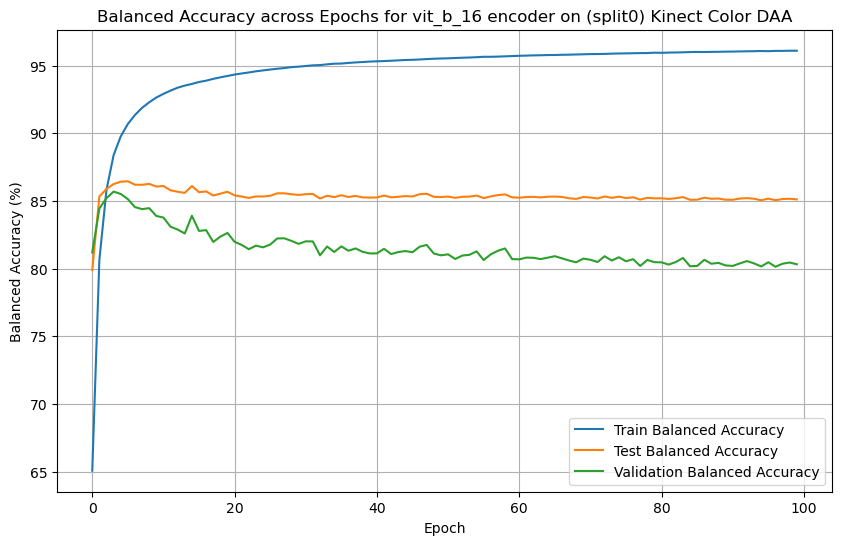
\includegraphics[width=\textwidth]{Images_Thesis/Tensboard_runs_images_all/Experiment_00_Sup_D_A_no_Aug/Split_0/output_bal_acc_no_aug.png}
        \caption{Split 0: Balanced Accuracy vs Epochs}
        \label{fig:Exp_1_01}
    \end{subfigure}
    \hfill % space between images
    \begin{subfigure}[b]{0.45\textwidth}
        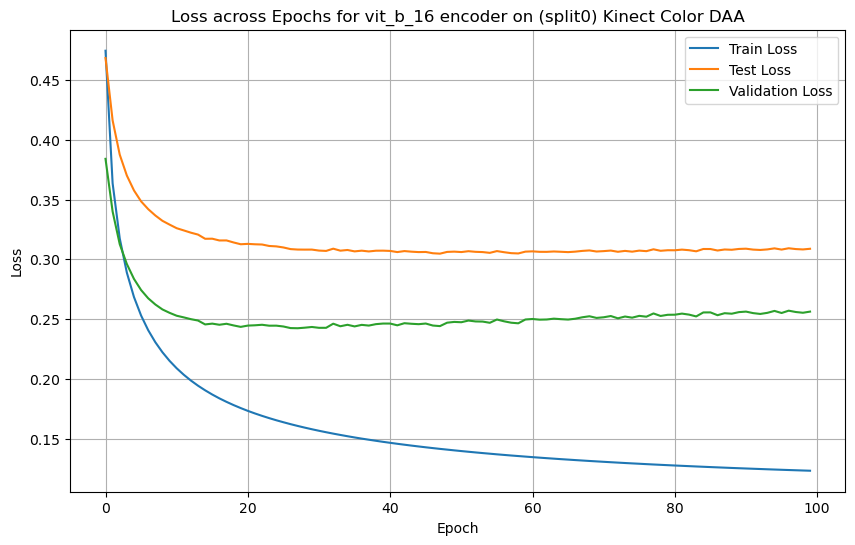
\includegraphics[width=\textwidth]{Images_Thesis/Tensboard_runs_images_all/Experiment_00_Sup_D_A_no_Aug/Split_0/output_loss_splt_0_no_aug_d_a.png}
        \caption{Split 0: Loss vs Epochs}
        \label{fig:Exp_1_02}
    \end{subfigure}

    % Second row
    \begin{subfigure}[b]{0.45\textwidth}
        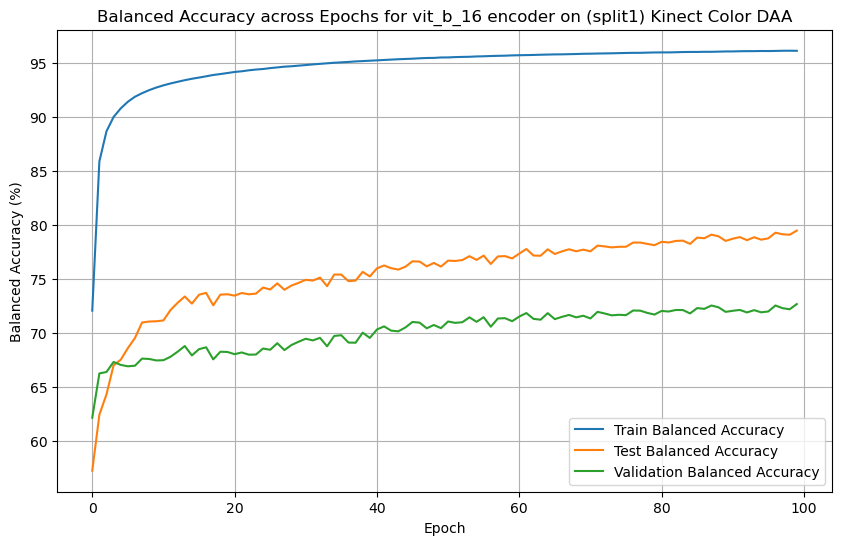
\includegraphics[width=\textwidth]{Images_Thesis/Tensboard_runs_images_all/Experiment_00_Sup_D_A_no_Aug/Split_1/output_bal_acc_d_a_no_aug.png}
        \caption{Split 1: Balanced Accuracy vs Epochs}
        \label{fig:Exp_1_03}
    \end{subfigure}
    \hfill
    \begin{subfigure}[b]{0.45\textwidth}
        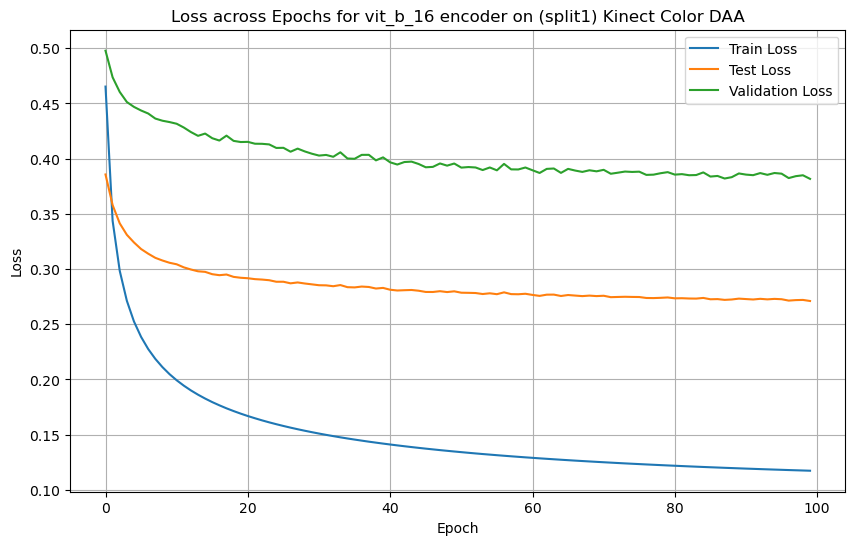
\includegraphics[width=\textwidth]{Images_Thesis/Tensboard_runs_images_all/Experiment_00_Sup_D_A_no_Aug/Split_1/output_loss_d_a_no_aug_split_1.png}
        \caption{Split 1:  Loss vs Epochs}
        \label{fig:Exp_1_04}
    \end{subfigure}

    % Third row
    \begin{subfigure}[b]{0.45\textwidth}
        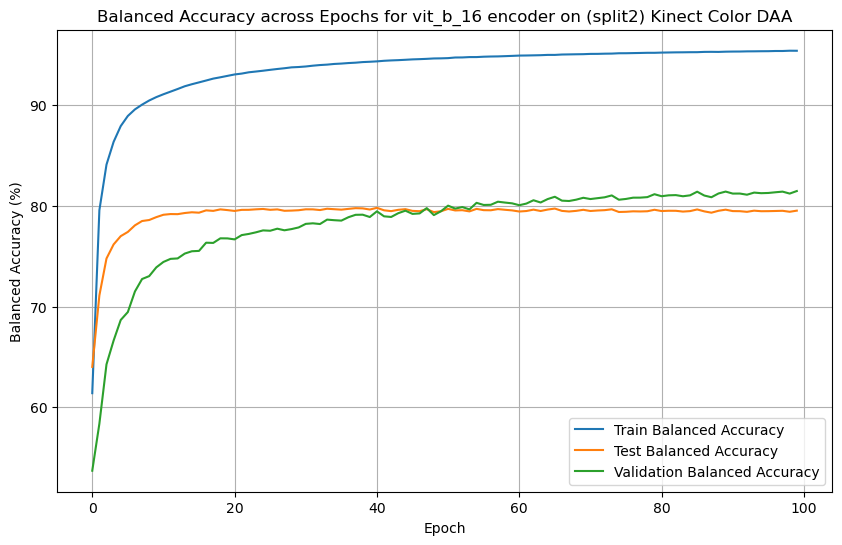
\includegraphics[width=\textwidth]{Images_Thesis/Tensboard_runs_images_all/Experiment_00_Sup_D_A_no_Aug/Split_2/output_bal_acc_split_2_d_a_no_aug.png}
        \caption{Split 2: Balanced Accuracy vs Epochs}
        \label{fig:Exp_1_05}
    \end{subfigure}
    \hfill
    \begin{subfigure}[b]{0.45\textwidth}
        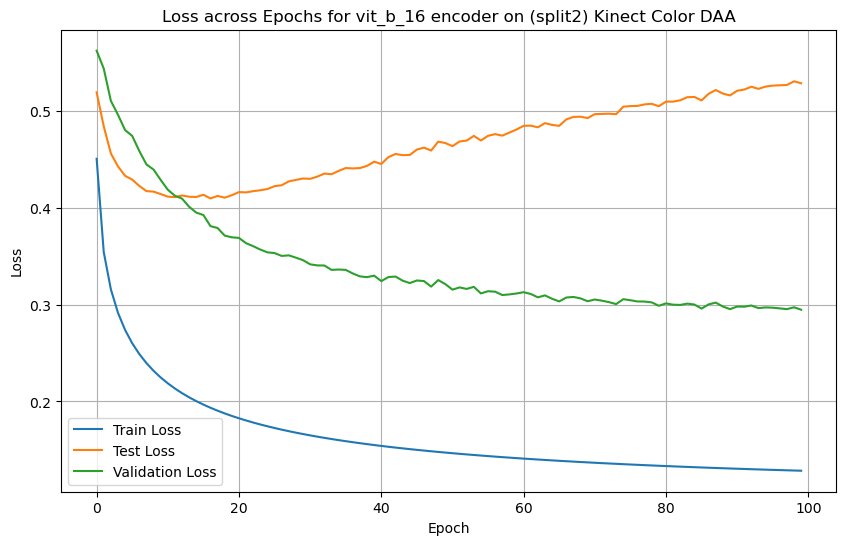
\includegraphics[width=\textwidth]{Images_Thesis/Tensboard_runs_images_all/Experiment_00_Sup_D_A_no_Aug/Split_2/output_loss_split_2_d_a_no_aug.png}
        \caption{Split 2: Loss vs Epochs}
        \label{fig:Exp_1_06}
    \end{subfigure}
    \caption[Results of Experiment 1: Supervised Learning Based Encoder]{Comparison of training and evaluation based on balanced accuracy an loss curves plotted across epochs for all three splits of Kinect Color Right Top view DAA Image dataset for supervised learning based encoder in experiment 1.}
    \label{fig:Exp_1_00}
\end{figure}

The average training balanced accuracy across all splits is notably high at 95.88\%, demonstrating the model's robust ability to learn from the training data. However, the validation balanced accuracies are considerably lower, averaging 78.16\%, which indicates overfitting. The average test accuracy is somewhat higher at 81.38\%, indicating a reasonable generalization to unseen data.

Validation-balanced accuracies are much lower than training-balanced accuracies, indicating that the model struggles to generalize across dataset subsets. This discrepancy may be due to the unique Kinect Color Right Top view image dataset or limits in the transferability of pre-trained features to driver distraction detection task and requires further research in this direction. Similarly, the significant difference between training and validation balanced accuracy in Table~\ref{table:experiment 1 results}, especially in Split 1, shows overfitting. 
%%%%%%%%%%%% Result table: Experiment 1 %%%%%%%%%%%
\begin{table}[htbp]
\caption[Results of experiment 1: supervised learning based encoder]{Supervised learning based encoder results on driver distraction detection task. The linear layer on top of pretrained frozen encoder (vit\_b\_16) is trained and evaluated on all three splits of Kinect Color Right Top DAA image dataset for 100 epochs using DDP algorithm on dual GPU setup with an effective batch of 1024. The results are avearged for 100th epoch for comparison with subsequent experiments.}
\label{table:experiment 1 results}
\centering
\begin{tabular}{lllllll}
\multicolumn{1}{c}{\textbf{Splits}} & \multicolumn{1}{c}{\textbf{View}} & \multicolumn{1}{c}{\textbf{Encoder}} & \multicolumn{1}{c}{\textbf{Epoch}} & \multicolumn{1}{c}{\textbf{Train}} & \multicolumn{1}{c}{\textbf{Val}} & \multicolumn{1}{c}{\textbf{Test}}\\
\hline
Split\_0 & Right Top & vit\_b\_16 & 100 & 96.10\% & 80.32\% & 85.12\% \\
Split\_1 & Right Top & vit\_b\_16 & 100 & 96.12\% & 72.69\% & 79.49\% \\
Split\_2 & Right Top & vit\_b\_16 & 100 & 95.42\% & 81.48\% & 79.53\% \\
\hline
Average & Right Top & vit\_b\_16 & 100 & 95.88\% & 78.16\% & 81.38\% \\
\hline
\end{tabular}
\end{table}

Figure~\ref{fig:Exp_1_00} shows this experiment's balanced accuracy and loss curves. It can be seen in the figure that each split exhibits high initial training balanced accuracies, quickly reaching a plateau. This behavior underscores the effective utilization of the pre-trained features of the ViT-B/16, which is adept at adapting quickly to the training data. However, the validation and test accuracies across the splits show varied patterns. Test-balanced accuracies generally stabilize at higher levels than validation, suggesting better generalization on the test set. Notably, Split 2 shows a closer convergence between validation and test balanced accuracies, indicating more effective generalization compared to Splits 0 and 1.

Similarly, the loss curves in the figure~\ref{fig:Exp_1_00} show sharp initial declines in training loss in all splits, reflecting efficient error minimization on training data. However, the validation loss behaviors vary, with Split 2 displaying an increasing trend after initial stabilization—signaling potential overfitting or inadequate model tuning for generalization.

The trained linear layer on top of the frozen supervised learning-based encoder (vit\_b\_16) in this experiment is further tested for cross-modality and cross-view generalization on the Kinect IR and NIR DAA test datasets across all splits, as described in sections~\ref{section:Methodology for Cross-Modality Generalization Evaluation} and~\ref{section:Methodology for Cross-View Generalization Evaluation}. Tables \ref{table:experiment 1 results Cross Modality Generalisation} and \ref{table:experiment 1 results Cross Modality and view Generalisation on NIR} shows the model's performance on Kinect IR and NIR DAA image datasets with different camera view and image modality than the training dataset.

%%% Cross Modality Generalisation Tables %%%%%%%%%%
\begin{table}[htbp]
\caption[Results of Experiment 1 for Cross Modality Generalisation]{Performance of the Linear Layer trained on top of the Frozen Supervised Encoder on Kinect IR Right Top View Dataset: This table shows the results from evaluating the 100th checkpoint of the model, initially trained on color images, on the grayscale test sets of the Kinect IR Right Top view dataset.}
\label{table:experiment 1 results Cross Modality Generalisation}
\centering
\begin{tabular}{lllll}
\multicolumn{1}{c}{\textbf{Splits}} & \multicolumn{1}{c}{\textbf{View}} & \multicolumn{1}{c}{\textbf{Encoder}} & \multicolumn{1}{c}{\textbf{Checkpoint}} & \multicolumn{1}{c}{\textbf{Test}}\\
\hline
Split\_0 & Right Top & vit\_b\_16 & 100 & 49.96\% \\
Split\_1 & Right Top & vit\_b\_16 & 100 & 57.83\% \\
Split\_2 & Right Top & vit\_b\_16 & 100 & 52.42\% \\
\hline
Average & KIR Right Top & vit\_b\_16 & 100 & 53.40\% \\
\hline
\end{tabular}
\end{table}

\textbf{Cross-Modality and Cross-View Generalization:}
The performance on the Kinect IR Right Top view dataset (Table \ref{table:experiment 1 results Cross Modality Generalisation}) shows that the model achieves an average test balanced accuracy of 53.40\%. This result is considerably lower than the training balanced accuracies observed on the Kincet Color DAA dataset, highlighting challenges in the model's ability to generalize to grayscale IR images. Individual splits show variability, with the highest being 57.83\% in Split 1 and the lowest at 49.96\% in Split 0, suggesting some inconsistency in the model's performance across different segments of the Kinect IR dataset.

Further evaluating the model's generalization capabilities, the NIR Front Top view dataset (Table \ref{table:experiment 1 results Cross Modality and view Generalisation on NIR}) shows even more uniform results with a narrow range of test balanced accuracies hovering around 49\%. The average balanced accuracy across the splits stands at 49.24\%, which is slightly lower than the Kinect IR dataset results. This indicates additional challenges when the model encounters not only a different modality but also a different viewing angle, emphasizing the specificity of the learned features to the training conditions.
%%% Cross Modality & Cross View Generalisation Tables %%%%%%%%%%
\begin{table}[htbp]
\caption[Results of Experiment 1 for Cross Modality and Cross view Generalisation.]{Performance of the Linear Layer trained on top of the Frozen Supervised Encoder on NIR Front Top View DAA Dataset: This table shows the results from evaluating the 100th checkpoint of the model, initially trained on color images, on the grayscale test sets of the NIR Front Top view dataset. Here model evaluation is performed on gray scale images and front top view resulting in cross-modality and cross-view generalization evaluation.}
\label{table:experiment 1 results Cross Modality and view Generalisation on NIR}
\centering
\begin{tabular}{lllll}
\multicolumn{1}{c}{\textbf{Splits}} & \multicolumn{1}{c}{\textbf{View}} & \multicolumn{1}{c}{\textbf{Encoder}} & \multicolumn{1}{c}{\textbf{Checkpoint}} & \multicolumn{1}{c}{\textbf{Test}}\\
\hline
Split\_0 & Front Top & vit\_b\_16 & 100 & 49.79\% \\
Split\_1 & Front Top & vit\_b\_16 & 100 & 49.53\% \\
Split\_2 & Front Top & vit\_b\_16 & 100 & 48.41\% \\
\hline
Average & NIR Front Top & vit\_b\_16 & 100 & 49.24\% \\
\hline
\end{tabular}
\end{table}

These results demonstrate the limitations of applying models trained on specific datasets and modalities to other dataset without adaptation or training. The model's feature extraction abilities appear to be highly related to the training data's features, as color to grayscale images and viewing perspectives significantly decrease performance. Domain adaptation, fine-tuning on target domain datasets, and more diversified training data including many modalities and perspectives may improve cross-modality and cross-view generalization. 

In conclusion, while the linear layer trained on top of frozen encoder vit\_b\_16 demonstrates robust learning capabilities within its training data modality, its application to significantly different data modality without prior adaptation highlights the critical need for models that better generalize across diverse input conditions. Further research into transfer learning and domain generalization techniques would be beneficial to address these challenges and improve the practical utility of such models in real-world applications like driver distraction detection.
%%%%%%%%%%%%%%%%%%%%%%%%%%%%%%%%%%%%%%%%%%%%%%%%%%%%%%%%%%%%%%
\subsection{Results of Experiment 2: Supervised Learning Based Encoder with Gray scale Augmentation}
The results of previous experiment show that without prior training on grayscale image data, the linear layer trained on top of a frozen supervised learning-based encoder (vit\_b\_16) does not generalize effectively on cross-modality and cross-view dataset images. This experiment uses the approach described in section~\ref{section:Methodology 2 Experiment 2: Supervised Learning Based Encoder with Gray scale Augmentation} to assess the model's generalization capabilities while providing grayscale transforms during training. This experiment employed the same training setup as experiment 1, with the main variation being that grayscale transforms were applied to the images fed into the model training. In other words, the color images in the Kinect Color Right Top view dataset are first transformed to grayscale before being given into the model for further training of the linear layer on top of the (vit\_b\_16) encoder. Table~\ref{table:experiment 2 results} summarizes the findings of this experiment.
%%%%%%%%%%%% Result table: Experiment 2 %%%%%%%%%%%
\begin{table}[htbp]
\caption{Results of Experiment 2: Supervised Learning Based Encoder with Gray scale augmentation}
\label{table:experiment 2 results}
\centering
\begin{tabular}{lllllll}
\multicolumn{1}{c}{\textbf{Splits}} & \multicolumn{1}{c}{\textbf{View}} & \multicolumn{1}{c}{\textbf{Augmentation}} & \multicolumn{1}{c}{\textbf{Encoder}} & \multicolumn{1}{c}{\textbf{Train}} & \multicolumn{1}{c}{\textbf{Val}} & \multicolumn{1}{c}{\textbf{Test}}\\
\hline
Split\_0 & Right Top & Gray Scale & vit\_b\_16 & 95.61\% & 68.43\% & 62.25\% \\
Split\_1 & Right Top & Gray Scale & vit\_b\_16 & 95.88\% & 64.28\% & 86.64\% \\
Split\_2 & Right Top & Gray Scale & vit\_b\_16 & 95.12\% & 87.73\% & 84.52\% \\
\hline
Average & Right Top & Gray Scale & vit\_b\_16 & 95.53\% & 73.48\% & 77.80\% \\
\hline
\end{tabular}
\end{table}

Table~\ref{table:experiment 2 results} shows a high average training balanced accuracy of 95.53\% across all splits, indicating the model's strong capacity to learn from augmented grayscale training data. However, the validation balanced accuracies are significantly lower, averaging 73.48 percent, indicating overfitting. The average test balanced accuracy is slightly better at 77.80\%, demonstrating a decent generalization to unseen augmented grayscale data. 

Validation-balanced accuracies are much lower than training-balanced accuracies, indicating that the model trained using grayscale augmentations struggles to generalize across dataset subsets except for split 2, where the validation-balanced accuracy, at 87.73\%, is slightly better than the other two splits. Similarly, the test-balanced accuracy for split 1 and split 2 are much higher than those for split 0.

%%%%%%%%%%%%%%%%%% Grid of class distributions %%%%%%%%%%%%%%%%%
\begin{figure}[htbp]
    \centering
    % First row
    \begin{subfigure}[b]{0.45\textwidth}
        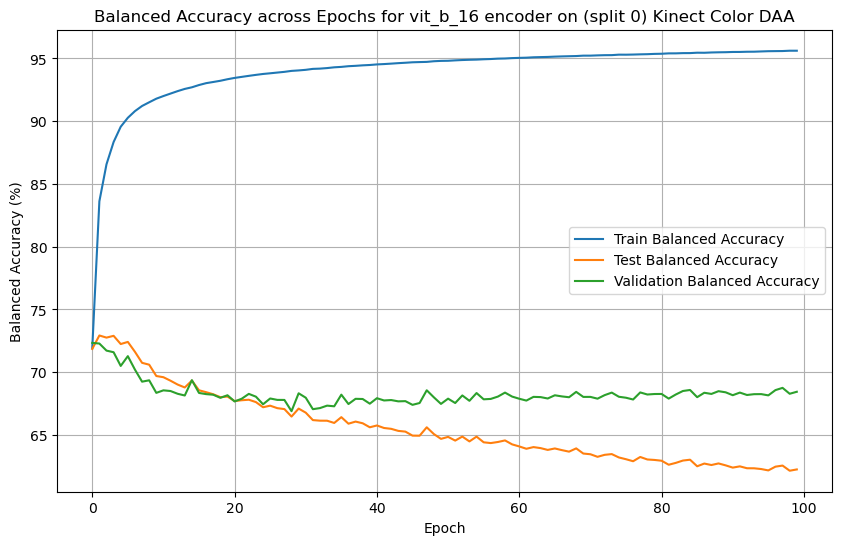
\includegraphics[width=\textwidth]{Images_Thesis/Tensboard_runs_images_all/Experiment_01_Sup_D_A_with_Aug/Split_0/output_bal_acc_split_0_with_aug_d_a.png}
        \caption{Split 0: Balanced Accuracy vs Epochs}
        \label{fig:Exp_2_01}
    \end{subfigure}
    \hfill % space between images
    \begin{subfigure}[b]{0.45\textwidth}
        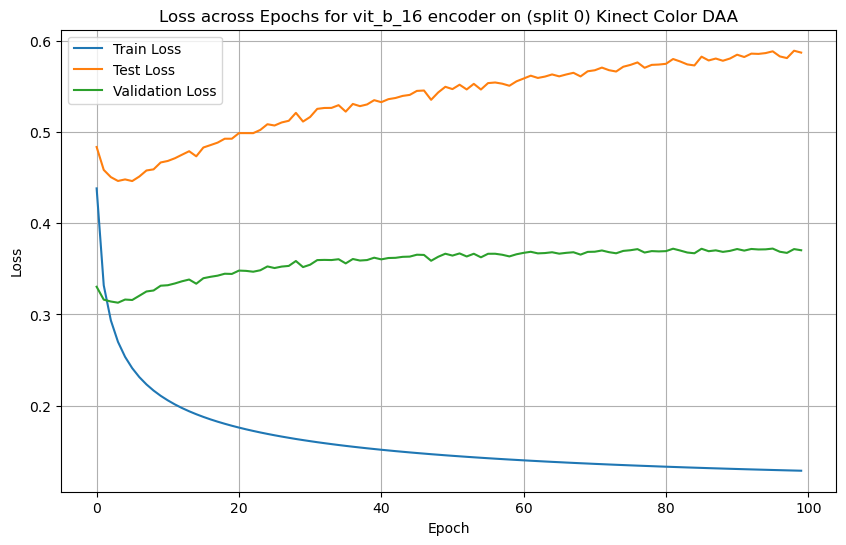
\includegraphics[width=\textwidth]{Images_Thesis/Tensboard_runs_images_all/Experiment_01_Sup_D_A_with_Aug/Split_0/output_loss_split_0_with_aug_d_a.png}
        \caption{Split 0: Loss vs Epochs}
        \label{fig:Exp_2_02}
    \end{subfigure}

    % Second row
    \begin{subfigure}[b]{0.45\textwidth}
        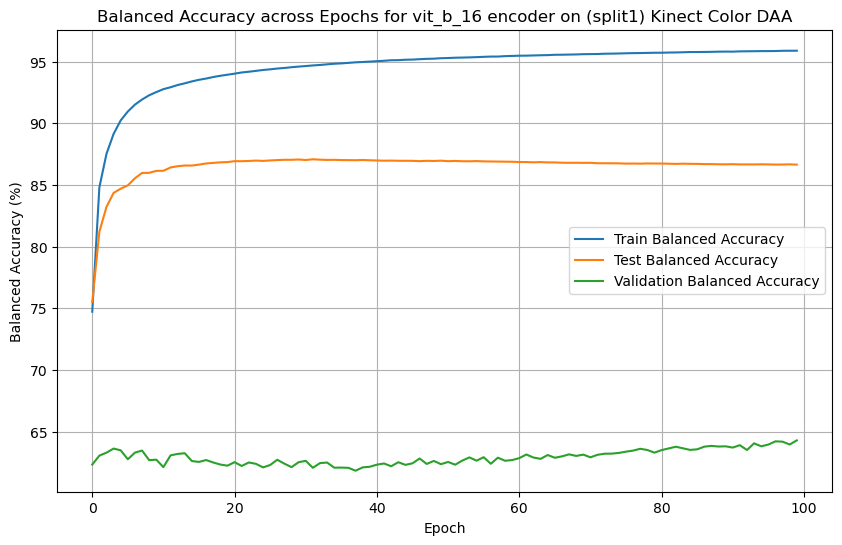
\includegraphics[width=\textwidth]{Images_Thesis/Tensboard_runs_images_all/Experiment_01_Sup_D_A_with_Aug/Split_1/output_bal_acc_split_1_with_aug_d_a.png}
        \caption{Split 1: Balanced Accuracy vs Epochs}
        \label{fig:Exp_2_03}
    \end{subfigure}
    \hfill
    \begin{subfigure}[b]{0.45\textwidth}
        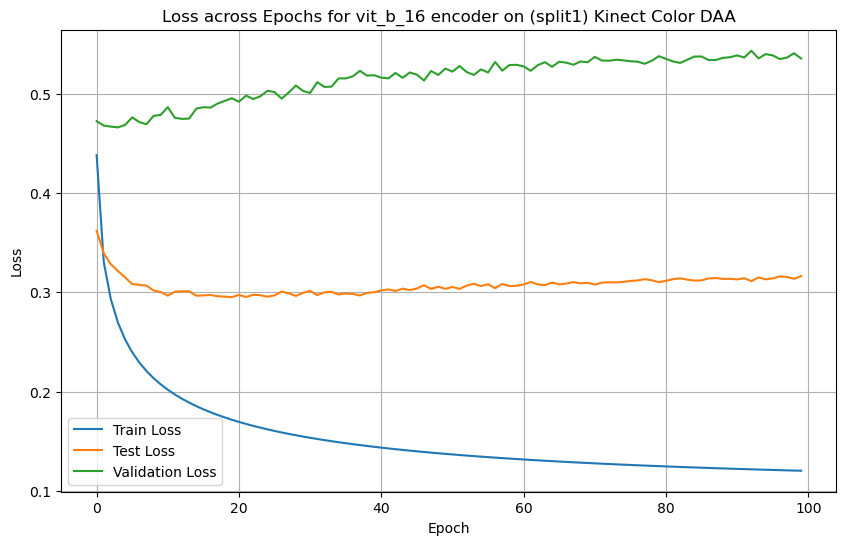
\includegraphics[width=\textwidth]{Images_Thesis/Tensboard_runs_images_all/Experiment_01_Sup_D_A_with_Aug/Split_1/output_loss_split_1_with_aug_d_a.png}
        \caption{Split 1:  Loss vs Epochs}
        \label{fig:Exp_2_04}
    \end{subfigure}

    % Third row
    \begin{subfigure}[b]{0.45\textwidth}
        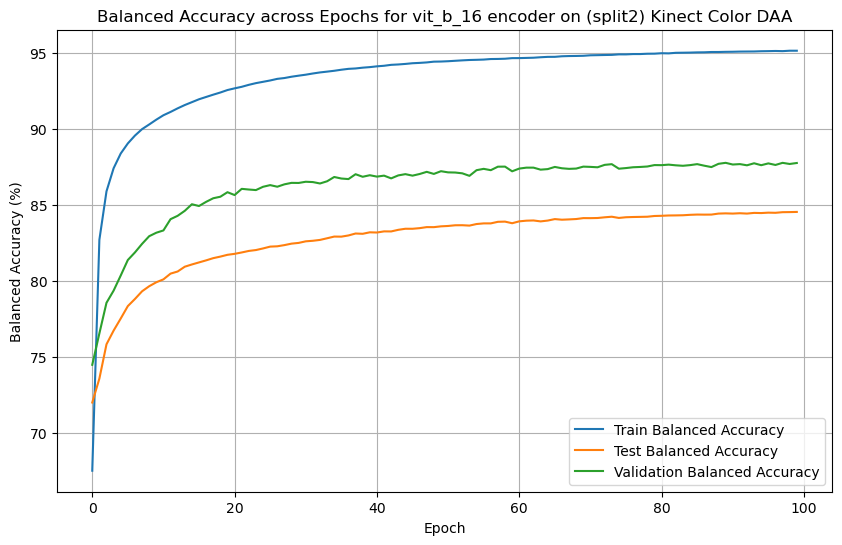
\includegraphics[width=\textwidth]{Images_Thesis/Tensboard_runs_images_all/Experiment_01_Sup_D_A_with_Aug/Split_2/output_bal_acc_split_2_with_aug_d_a.png}
        \caption{Split 2: Balanced Accuracy vs Epochs}
        \label{fig:Exp_2_05}
    \end{subfigure}
    \hfill
    \begin{subfigure}[b]{0.45\textwidth}
        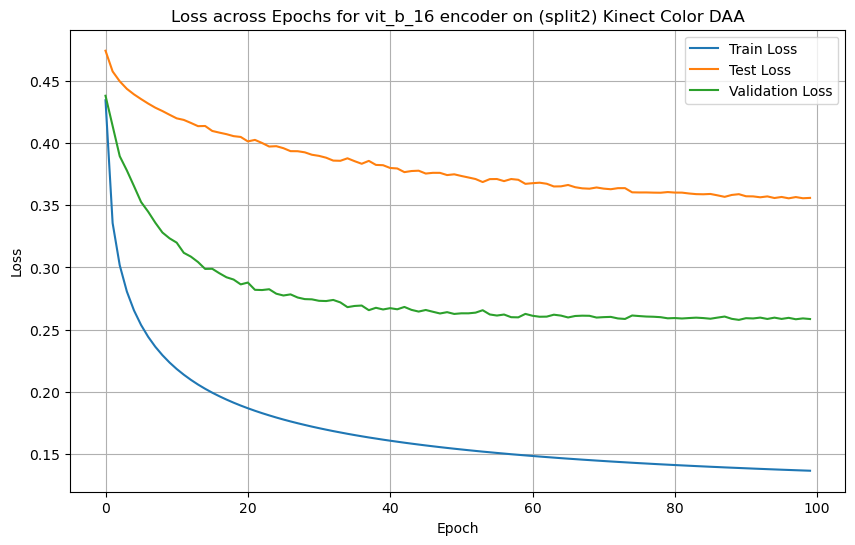
\includegraphics[width=\textwidth]{Images_Thesis/Tensboard_runs_images_all/Experiment_01_Sup_D_A_with_Aug/Split_2/output_loss_split_2_with_aug_d_a.png}
        \caption{Split 2: Loss vs Epochs}
        \label{fig:Exp_2_06}
    \end{subfigure}
    \caption[Results of Experiment 2: Supervised Learning Based Encoder with Gray Scale Augmentation]{Comparison of training and evaluation based on balanced accuracy an loss curves plotted across epochs for all three splits of Kinect Color Right Top view DAA Image dataset for supervised learning based encoder  with Gray Scale Augmentation in experiment 2.}
    \label{fig:Exp_2_00}
\end{figure}

Figure~\ref{fig:Exp_2_00} depicts the balanced accuracy and loss curves from this experiment. The figure shows that each split demonstrates high initial training balanced accuracies before shortly plateauing. This behavior highlights the effective exploitation of the pre-trained features of the vit\_b\_16 encoder, which can quickly adjust to the augmented training data. However, the validation and test accuracies throughout the splits exhibit different patterns. Split 1 test-balanced accuracy tends to stabilize at a greater level than validation.
On the contrary, for split 2, validation-balanced accuracy stabilizes at a higher level than the test. For split 1, both validation and test-balanced accuracies show a decreasing trend, which indicates overfitting. Notably, Split 2 shows better convergence for validation and test-balanced accuracies, indicating more effective generalization compared to splits 0 and 1.

The loss curves in Figure~\ref{fig:Exp_2_00} show sharp early drops in training loss in all splits, indicating efficient error minimization on the augmented grayscale training data. However, the validation loss (green) behaviors differ, with Split 1 showing an increasing trend from the start, indicating potential overfitting. On the other hand, for split 1, the test loss (orange) curve is much better and much closer to the train loss curve than the validation loss curve. In the split 0 loss curve plot, the test loss curve increases after the first few epochs, indicating poor generalization, as shown in the split 0 balanced accuracy plot. 


Like the last, this experiment evaluates the model trained on a grayscale augmented Kinect Color Right Top DAA image dataset across cross-modality and views. The data sets utilized for this evaluation are identical to those used in previous experiment. Tables \ref{table:experiment 2 results Cross Modality Generalisation} and \ref{table:experiment 2 results Cross Modality and view Generalisation on NIR} demonstrate the model's performance on the Kinect IR and NIR DAA image datasets. 
%%% Cross Modality Generalisation Tables %%%%%%%%%%
\begin{table}[htbp]
\caption{Results of Experiment 2 for Cross Modality Generalisation on test sets of Kinect IR DAA Image Dataset}
\label{table:experiment 2 results Cross Modality Generalisation}
\centering
\begin{tabular}{lllll}
\multicolumn{1}{c}{\textbf{Splits}} & \multicolumn{1}{c}{\textbf{View}} & \multicolumn{1}{c}{\textbf{Encoder}} & \multicolumn{1}{c}{\textbf{Checkpoint}} & \multicolumn{1}{c}{\textbf{Test}}\\
\hline
Split\_0 & Right Top & vit\_b\_16 & 100 & 50.58\% \\
Split\_1 & Right Top & vit\_b\_16 & 100 & 53.34\% \\
Split\_2 & Right Top & vit\_b\_16 & 100 & 60.66\% \\
\hline
Average & KIR Right Top & vit\_b\_16 & 100 & 54.86\% \\
\hline
\end{tabular}
\end{table}

%%% Cross Modality & Cross View Generalisation Tables %%%%%%%%%%
\begin{table}[htbp]
\caption{Results of Experiment 2 for Cross Modality and Cross view Generalisation on test sets of NIR DAA Image Dataset}
\label{table:experiment 2 results Cross Modality and view Generalisation on NIR}
\centering
\begin{tabular}{lllll}
\multicolumn{1}{c}{\textbf{Splits}} & \multicolumn{1}{c}{\textbf{View}} & \multicolumn{1}{c}{\textbf{Encoder}} & \multicolumn{1}{c}{\textbf{Checkpoint}} & \multicolumn{1}{c}{\textbf{Test}}\\
\hline
Split\_0 & Front Top & vit\_b\_16 & 100 & 49.68\% \\
Split\_1 & Front Top & vit\_b\_16 & 100 & 49.97\% \\
Split\_2 & Front Top & vit\_b\_16 & 100 & 49.17\% \\
\hline
Average & NIR Front Top & vit\_b\_16 & 100 & 49.60\% \\
\hline
\end{tabular}
\end{table}

\textbf{Cross-modality and cross-view generalization:}
The performance on the Kinect IR Right Top view dataset (Table \ref{table:experiment 2 results Cross Modality Generalisation}) shows that the model achieves an average test balanced accuracy of 54.86\%. This result is considerably lower than the train and test balanced accuracies observed on the augmented Kinect Color DAA dataset. However, compared to the cross-modality generalization results from experiment 1 on the Kinect IR Right Top dataset, there is an increment of 1.46\% from 53.40\% to 54.86\%. This slight increment highlights the model's challenges in generalizing to grayscale IR images. Individual splits show variability, with the highest being 60.66\% in Split 2 and the lowest at 50.58\% in Split 0, suggesting some inconsistency in the model's performance across different segments of the Kinect IR dataset.

The NIR Front Top view dataset (Table \ref{table:experiment 2 results Cross Modality and view Generalisation on NIR}) demonstrates consistent results with test balanced accuracies around 49\%. The average balanced accuracy across splits is 49.60\%, somewhat higher than experiment 1 findings on the NIR Front top view DAA dataset. This finding suggests that cross-view generalization remains challenging when the model faces a new viewing angle, stressing the relevance of the learnt features in the pre-trained encoders to the training conditions.
This also emphasizes the importance of a foundational vision model for such complicated generalization tasks, which leads this thesis to encoders trained utilizing self-supervised learning approaches on huge curated datasets without labels, as done in the~\citep{dinov2_oquab2023dinov2}.
%%%%%%%%%%%%%%%%%%%%%%%%%%%%%%%%%%%%%%%%%%%%%%%%%%%%%%%%%%%%%%
\subsection{Results of Experiment 3: Self-Supervised Learning Based Encoder}
%%%%%%%%%%%%%%%%%%%%%%%%%Text Here%%%%%%%%%%%%%%%%%%%%%%%%%%%%
As demonstrated by the results of experiment 2, by providing prior knowledge about the modality, such as augmenting color images to grayscale prior to model training, we can progress toward increasing cross-modality generalization to some extent; however, cross-view generalization still requires a robust encoder whose knowledge can be transferred to the cross-view generalization. Following the methodology in section~\ref{section:Methodology Experiment 3: Self-Supervised Learning Based Encoder}, in this experiment, we have replaced the supervised encoder with the self-supervised encoder (vit\_b\_14), which is trained using the DINOv2~\citep{dinov2_oquab2023dinov2} self-supervised learning approach on a huge curated dataset LVD-142M~\citep{dinov2_oquab2023dinov2} with 142 million images without labels. This experiment's setup is identical to that of experiment 1, using the same hyperparameters to provide a fair performance comparison.

%%%%%%%%%%%%%%%%%% Grid of class distributions %%%%%%%%%%%%%%%%%
\begin{figure}[htbp]
    \centering
    % First row
    \begin{subfigure}[b]{0.45\textwidth}
        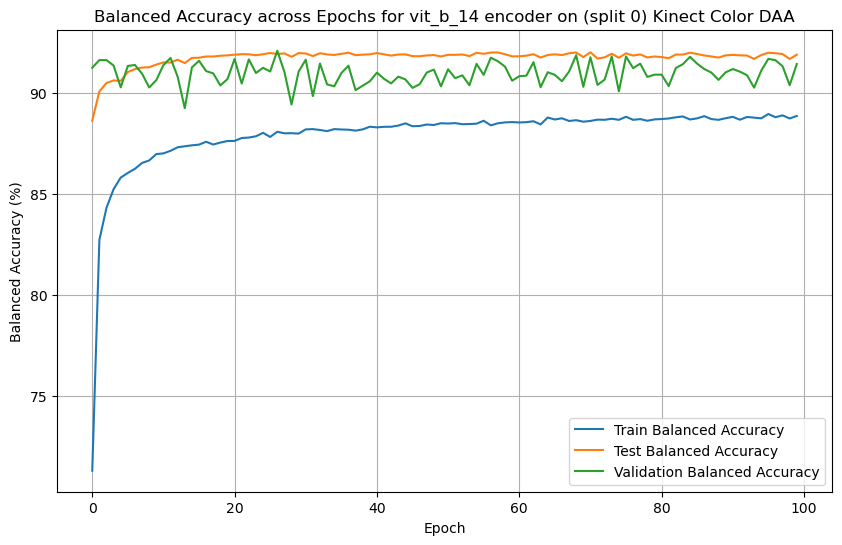
\includegraphics[width=\textwidth]{Images_Thesis/Tensboard_runs_images_all/Experiment_02_Sel_Sup_D_A_no_Aug/Split_0/output_bal_acc_split_0_d_a_ssl.png}
        \caption{Split 0: Balanced Accuracy vs Epochs}
        \label{fig:Exp_3_01}
    \end{subfigure}
    \hfill % space between images
    \begin{subfigure}[b]{0.45\textwidth}
        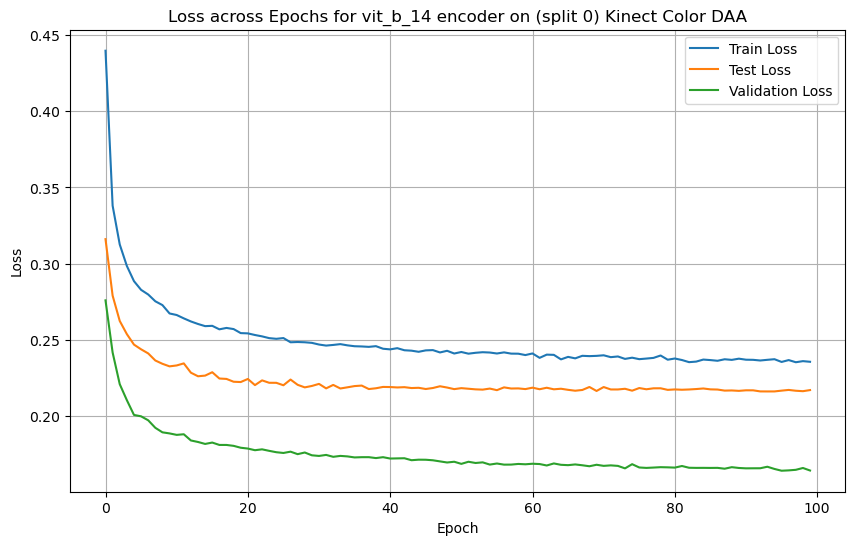
\includegraphics[width=\textwidth]{Images_Thesis/Tensboard_runs_images_all/Experiment_02_Sel_Sup_D_A_no_Aug/Split_0/output_loss_split_0_d_a_ssl.png}
        \caption{Split 0: Loss vs Epochs}
        \label{fig:Exp_3_02}
    \end{subfigure}

    % Second row
    \begin{subfigure}[b]{0.45\textwidth}
        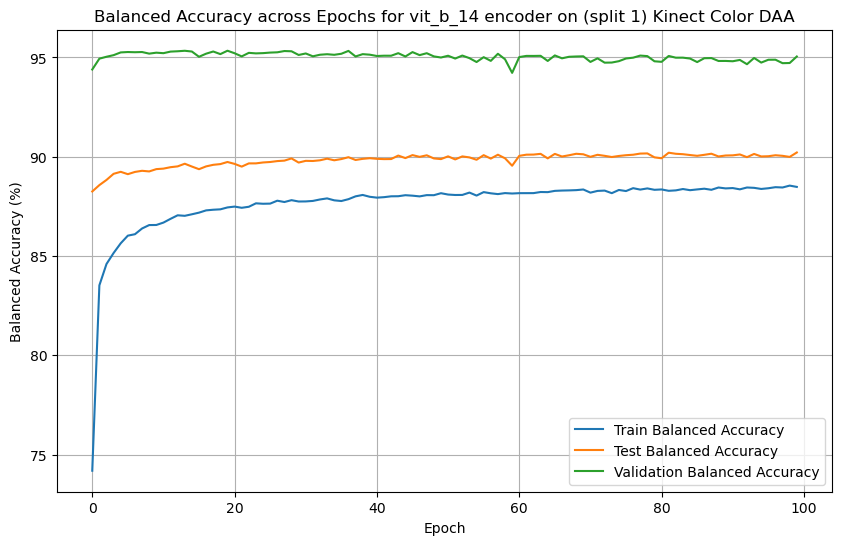
\includegraphics[width=\textwidth]{Images_Thesis/Tensboard_runs_images_all/Experiment_02_Sel_Sup_D_A_no_Aug/Split_1/output_bal_acc_split_1_d_a_ssl.png}
        \caption{Split 1: Balanced Accuracy vs Epochs}
        \label{fig:Exp_3_03}
    \end{subfigure}
    \hfill
    \begin{subfigure}[b]{0.45\textwidth}
        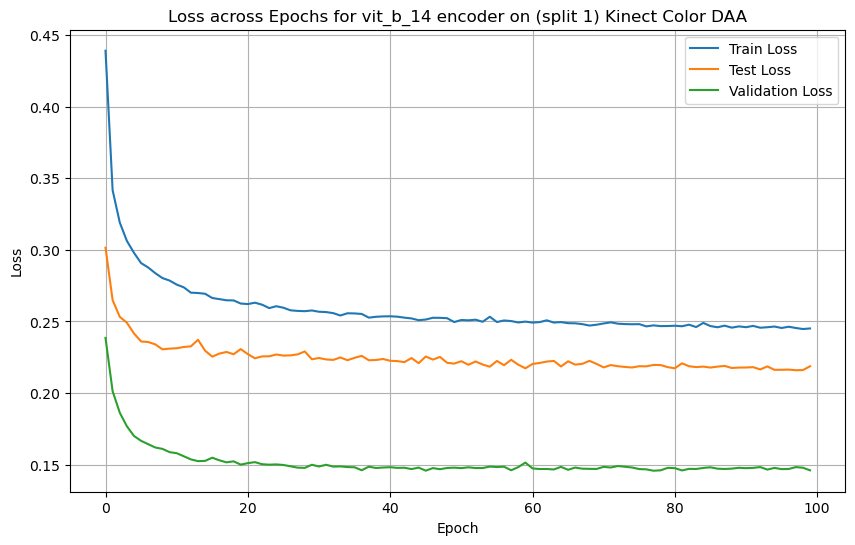
\includegraphics[width=\textwidth]{Images_Thesis/Tensboard_runs_images_all/Experiment_02_Sel_Sup_D_A_no_Aug/Split_1/output_loss_split_1_d_a_ssl.png}
        \caption{Split 1:  Loss vs Epochs}
        \label{fig:Exp_3_04}
    \end{subfigure}

    % Third row
    \begin{subfigure}[b]{0.45\textwidth}
        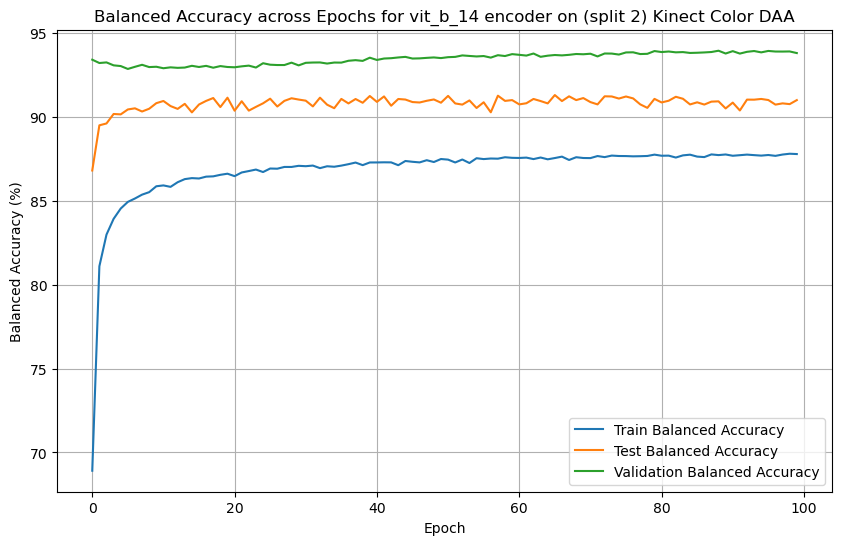
\includegraphics[width=\textwidth]{Images_Thesis/Tensboard_runs_images_all/Experiment_02_Sel_Sup_D_A_no_Aug/Split_2/output_bal_acc_split_2_d_a_ssl.png}
        \caption{Split 2: Balanced Accuracy vs Epochs}
        \label{fig:Exp_3_05}
    \end{subfigure}
    \hfill
    \begin{subfigure}[b]{0.45\textwidth}
        \includegraphics[width=\textwidth]{Images_Thesis/Tensboard_runs_images_all/Experiment_02_Sel_Sup_D_A_no_Aug/Split_2/output_loss_split_2_d_a_ssl.png}
        \caption{Split 2: Loss vs Epochs}
        \label{fig:Exp_3_06}
    \end{subfigure}
    \caption[Results of Experiment 3: Self Supervised Learning Based Encoder]{Comparison of training and evaluation based on balanced accuracy an loss curves plotted across epochs for all three splits of Kinect Color Right Top view DAA Image dataset for self supervised learning based encoder in experiment 3.}
    \label{fig:Exp_3_00}
\end{figure}

Table~\ref{table:experiment 3 results} shows an average training balanced accuracy of 88.36\% across all splits, indicating the model's strong capacity to learn from Kinect Right Top view color training data. However, the validation balanced accuracies are significantly higher, averaging 93.42 percent, indicating underfitting. The average test-balanced accuracy is slightly lower than validation-balanced accuracy at 91.02\%, demonstrating a decent generalization to unseen data.
%%%%%%%%%%%% Result table: Experiment 3 %%%%%%%%%%%
\begin{table}[htbp]
\caption{Results of Experiment 3: Self-Supervised Learning Based Encoder}
\label{table:experiment 3 results}
\centering
\begin{tabular}{llllll}
\multicolumn{1}{c}{\textbf{Splits}} & \multicolumn{1}{c}{\textbf{View}} & \multicolumn{1}{c}{\textbf{Encoder}} & \multicolumn{1}{c}{\textbf{Train}} & \multicolumn{1}{c}{\textbf{Val}} & \multicolumn{1}{c}{\textbf{Test}}\\
\hline
Split\_0 & Right Top & DINOv2\_vit\_b\_14 & 88.83\% & 91.41\% & 91.87\% \\
Split\_1 & Right Top & DINOv2\_vit\_b\_14 & 88.48\% & 95.04\% & 90.21\% \\
Split\_2 & Right Top & DINOv2\_vit\_b\_14 & 87.79\% & 93.81\% & 91.00\% \\
\hline
Average & Right Top & DINOv2\_vit\_b\_14 & 88.36\% & 93.42\% & 91.02\% \\
\hline
\end{tabular}
\end{table}

Validation-balanced accuracies are much higher than training-balanced accuracies, indicating that the model trained using Kinect color right top view dataset generalizes across the dataset well. Similarly, the test-balanced accuracy also supports this argument by showing higher test-balanced accuracies than the training-balanced accuracies across all splits for the Kinect color right top view dataset. Figure~\ref{fig:Exp_3_00} depicts the balanced accuracy and loss curves from this experiment. The figure shows that each split demonstrates high initial validation and test balanced accuracies before shortly plateauing. 

The train balanced accuracy curves in the figure~\ref{fig:Exp_3_00} for all three splits reveals that although the model is underfitting, there is a lot higher generalization on unseen test data than in the prior two experiments. This demonstrates the robustness and powerful features that the DINOv2-based vit\_b\_14 encoder has. The loss curves in the figure~\ref{fig:Exp_3_00} also support the underfitting on all three splits. This suggests the need for different hyperparameter configurations for this experiment, which contributes to the future scope of this thesis.

Similar to the earlier two experiments, this experiment evaluates the model trained on a Kinect Color Right Top view DAA image dataset across cross-modality and views. The data sets utilized for this evaluation are identical to those used in earlier two experiments. Tables \ref{table:experiment 3 results Cross Modality Generalisation} and \ref{table:experiment 3 results Cross Modality and view Generalisation on NIR} demonstrate the model's performance on the Kinect IR and NIR DAA image datasets.

\textbf{Cross-Modality and Cross-View Generalization:}
The performance on the Kinect IR Right Top view dataset (Table \ref{table:experiment 3 results Cross Modality Generalisation}) shows that the model achieves an average test balanced accuracy of 60.57\%. This result is considerably lower than the test balanced accuracies observed on the Kinect Color Right Top view DAA dataset. However, compared to the cross-modality generalization results from experiment 1 and experiment 2 on the Kinect IR Right Top view dataset, there is an increment of 7.17\% from 53.40\% in experiment to 60.57\% in experiment 3 and 5.71\% from 54.86\% in experiment 1 to 60.57\% in experiment 3. This shows the superiority of the self-supervised learning-based encoder over the supervised learning-based encoder under consideration in this thesis on cross-modality generalization.
%%%%%%%%%%%%%%%%%%%%%%%%%%%%%%%%%%%%%%%%%%%%%%%%%%%%%%%%%%%%%%
%%% Cross Modality Generalisation Tables %%%%%%%%%%
\begin{table}[htbp]
\caption{Results of Experiment 3 for Cross Modality Generalisation on test sets of Kinect IR DAA Image Dataset}
\label{table:experiment 3 results Cross Modality Generalisation}
\centering
\begin{tabular}{lllll}
\multicolumn{1}{c}{\textbf{Splits}} & \multicolumn{1}{c}{\textbf{View}} & \multicolumn{1}{c}{\textbf{Encoder}} & \multicolumn{1}{c}{\textbf{Checkpoint}} & \multicolumn{1}{c}{\textbf{Test}}\\
\hline
Split\_0 & Right Top & DINOv2\_vit\_b\_14 & 100 & 71.80\% \\
Split\_1 & Right Top & DINOv2\_vit\_b\_14 & 100 & 56.64\% \\
Split\_2 & Right Top & DINOv2\_vit\_b\_14 & 100 & 53.27\% \\
\hline
Average & KIR Right Top & DINOv2\_vit\_b\_14 & 100 & 60.57\% \\
\hline
\end{tabular}
\end{table}

%%% Cross Modality & Cross View Generalisation Tables %%%%%%%%%%
\begin{table}[htbp]
\caption{Results of Experiment 3 for Cross Modality and Cross view Generalisation on test sets of NIR DAA Image Dataset}
\label{table:experiment 3 results Cross Modality and view Generalisation on NIR}
\centering
\begin{tabular}{lllll}
\multicolumn{1}{c}{\textbf{Splits}} & \multicolumn{1}{c}{\textbf{View}} & \multicolumn{1}{c}{\textbf{Encoder}} & \multicolumn{1}{c}{\textbf{Checkpoint}} & \multicolumn{1}{c}{\textbf{Test}}\\
\hline
Split\_0 & Front Top & DINOv2\_vit\_b\_14 & 100 & 50.05\% \\
Split\_1 & Front Top & DINOv2\_vit\_b\_14 & 100 & 51.10\% \\
Split\_2 & Front Top & DINOv2\_vit\_b\_14 & 100 & 50.49\% \\
\hline
Average & NIR Front Top & DINOv2\_vit\_b\_14 & 100 & 50.54\% \\
\hline
\end{tabular}
\end{table}

Further evaluating the model's generalization capabilities, the NIR Front Top view dataset (Table \ref{table:experiment 3 results Cross Modality and view Generalisation on NIR}) shows test balanced accuracies hovering around 50\%. The average balanced accuracy across the splits on the NIR Front top view DAA dataset stands at 50.54\%, which is 1.3\% greater than the one in experiment 1 and 0.94\% greater than the one in experiment 2. However, no significant improvement has been obtained, even using a very powerful encoder on cross-view and cross-modality generalization on the NIR Front Top view dataset. This shows that in order to improve the cross-view and cross-modality generalization on the NIR Front Top view dataset, the model needs prior training on the train sets of this dataset. To further enhance the performance on the NIR Front Top view dataset, the encoder can be completely fine-tuned on the datasets by unfreezing its pre-trained parameters for training, which will be computationally expensive given the large size and three splits of the \gls{daa} datasets.

\subsection{Results of Experiment 4: Self-Supervised Learning Based Encoder with Clustered Feature Weighting Data-loading}
%%%%%%%%%%%%%%%%%%%%%%%%%Text Here%%%%%%%%%%%%%%%%%%%%%%%%%%%%
In our previous three experiments, we assessed the efficacy of various training paradigms using a pre-trained vision transformer encoder obtained from supervised and self-supervised learning paradigms. The experiments examined the impact of pre-trained encoders on driver distraction detection. The datasets considered in this thesis were analyzed from a cross-modality and cross-view generalization perspective for driver distraction detection, utilizing the traditional imbalanced data-loading approach.

%%%%%%%%%%%%%%%%%% Grid of class distributions %%%%%%%%%%%%%%%%%
\begin{figure}[htbp]
    \centering
    % First row
    \begin{subfigure}[b]{0.45\textwidth}
        \includegraphics[width=\textwidth]{Images_Thesis/Tensboard_runs_images_all/Experiment_03_Sel_Sup_D_B_no_Aug/Split_0/output_bal_acc_split_0_d_b_ssl.png}
        \caption{Split 0: Balanced Accuracy vs Epochs}
        \label{fig:Exp_4_01}
    \end{subfigure}
    \hfill % space between images
    \begin{subfigure}[b]{0.45\textwidth}
        \includegraphics[width=\textwidth]{Images_Thesis/Tensboard_runs_images_all/Experiment_03_Sel_Sup_D_B_no_Aug/Split_0/output_loss_split_0_d_b_ssl.png}
        \caption{Split 0: Loss vs Epochs}
        \label{fig:Exp_4_02}
    \end{subfigure}

    % Second row
    \begin{subfigure}[b]{0.45\textwidth}
        \includegraphics[width=\textwidth]{Images_Thesis/Tensboard_runs_images_all/Experiment_03_Sel_Sup_D_B_no_Aug/Split_1/output_bal_acc_split_1_d_b_ssl.png}
        \caption{Split 1: Balanced Accuracy vs Epochs}
        \label{fig:Exp_4_03}
    \end{subfigure}
    \hfill
    \begin{subfigure}[b]{0.45\textwidth}
        \includegraphics[width=\textwidth]{Images_Thesis/Tensboard_runs_images_all/Experiment_03_Sel_Sup_D_B_no_Aug/Split_1/output_loss_split_1_d_b_ssl.png}
        \caption{Split 1:  Loss vs Epochs}
        \label{fig:Exp_4_04}
    \end{subfigure}

    % Third row
    \begin{subfigure}[b]{0.45\textwidth}
        \includegraphics[width=\textwidth]{Images_Thesis/Tensboard_runs_images_all/Experiment_03_Sel_Sup_D_B_no_Aug/Split_2/output_bal_acc_split_2_d_b_ssl.png}
        \caption{Split 2: Balanced Accuracy vs Epochs}
        \label{fig:Exp_4_05}
    \end{subfigure}
    \hfill
    \begin{subfigure}[b]{0.45\textwidth}
        \includegraphics[width=\textwidth]{Images_Thesis/Tensboard_runs_images_all/Experiment_03_Sel_Sup_D_B_no_Aug/Split_2/output_loss_split_2_d_b_ssl.png}
        \caption{Split 2: Loss vs Epochs}
        \label{fig:Exp_4_06}
    \end{subfigure}
    \caption[Results of Experiment 4: Self Supervised Learning Based Encoder with Clustered Feature Weighting Data-loading]{Comparison of training and evaluation based on balanced accuracy an loss curves plotted across epochs for all three splits of Kinect Color Right Top view DAA Image dataset for self supervised learning based encoder with Clustered Feature Weighting Data-loading in experiment 4.}
    \label{fig:Exp_4_00}
\end{figure}

Nevertheless, this thesis suggests a data loading approach called ``Clustered Feature Weighting" to enhance the imbalance in loading data in batches. This experiment evaluates the impact of modifying the dataloading strategy on driver distraction detection performance. Specifically, it focuses on three aspects: the driver distraction detection performance on the Kinect Color Right Top view DAA image dataset, the cross-modality generalization for driver distraction detection on the Kinect IR Right Top view DAA image dataset, and the cross-view and cross-modality generalization for driver distraction detection on the NIR Front Top-view DAA image dataset.

So, following the methodology in section~\ref{section: Methodology Experiment 4: Self-Supervised Learning Based Encoder with Clustered Feature Weighting Data-loading}, we have used clustered feature data loading with the self-supervised encoder (vit\_b\_14) in this experiment. This experiment's setup is identical to that of experiment 1, using the same hyperparameters to provide a fair performance comparison.
%%%%%%%%%%%% Result table: Experiment 4 %%%%%%%%%%%
\begin{table}[htbp]
\caption{Results of Experiment 4: Self-Supervised Learning Based Encoder with Clustered Feature Weighting Data-loading}
\label{table:experiment 4 results}
\centering
\begin{tabular}{llllll}
\multicolumn{1}{c}{\textbf{Splits}} & \multicolumn{1}{c}{\textbf{View}} & \multicolumn{1}{c}{\textbf{Encoder}} & \multicolumn{1}{c}{\textbf{Train}} & \multicolumn{1}{c}{\textbf{Val}} & \multicolumn{1}{c}{\textbf{Test}}\\
\hline
Split\_0 & Right Top & DINOv2\_vit\_b\_14 & 89.61\% & 92.91\% & 91.62\% \\
Split\_1 & Right Top & DINOv2\_vit\_b\_14 & 89.38\% & 95.32\% & 90.02\% \\
Split\_2 & Right Top & DINOv2\_vit\_b\_14 & 89.20\% & 93.55\% & 91.79\% \\
\hline
Average & Right Top & DINOv2\_vit\_b\_14 & 89.39\% & 93.92\% & 91.14\% \\
\hline
\end{tabular}
\end{table}

Table~\ref{table:experiment 4 results} shows driver distraction detection performance on the Kinect Color Right Top view dataset with an average training balanced accuracy of 89.39\% across all splits with an improvement of 1.03\% from experiment 3.The validation balanced accuracies average 93.92 percent,  indicating underfitting using novel data-loading, too. The balanced accuracy and loss curves in figure~\ref{fig:Exp_4_00} further confirm the phenomenon of underfitting. The average test-balanced accuracy is slightly lower than validation-balanced accuracy at 91.14\%, demonstrating a decent generalization to unseen test set data of Kinect Color dataset. In comparison to experiment 3, the train balanced accuracy in this experiment on the Kinect Color Right Top view dataset is 1.03\% higher. Additionally, the validation balanced accuracy is 0.5\% higher, and the test balanced accuracy is 0.08\% higher than in experiment 3. These results indicate that the model requires different hyperparameter configuration to prevent underfitting and assess the overall effectiveness and limitations of the `Clustered Feature Weighting' data-loading technique on the model's performance on driver distraction detection task.    

\textbf{Cross-Modality and Cross-View Generalization:}
The performance on the Kinect IR Right Top view dataset (Table \ref{table:experiment 4 results Cross Modality Generalisation}) shows that the model achieves an average test balanced accuracy of 54.37\%. 
%%% Cross Modality Generalisation Tables %%%%%%%%%%
\begin{table}[htbp]
\caption{Results of Experiment 4 for Cross Modality Generalization on test sets of Kinect IR DAA Image Dataset}
\label{table:experiment 4 results Cross Modality Generalisation}
\centering
\begin{tabular}{lllll}
\multicolumn{1}{c}{\textbf{Splits}} & \multicolumn{1}{c}{\textbf{View}} & \multicolumn{1}{c}{\textbf{Encoder}} & \multicolumn{1}{c}{\textbf{Checkpoint}} & \multicolumn{1}{c}{\textbf{Test}}\\
\hline
Split\_0 & Right Top & DINOv2\_vit\_b\_14 & 100 & 59.57\% \\
Split\_1 & Right Top & DINOv2\_vit\_b\_14 & 100 & 52.75\% \\
Split\_2 & Right Top & DINOv2\_vit\_b\_14 & 100 & 50.81\% \\
\hline
Average & KIR Right Top & DINOv2\_vit\_b\_14 & 100 & 54.37\% \\
\hline
\end{tabular}
\end{table}

%%% Cross Modality & Cross View Generalisation Tables %%%%%%%%%%
\begin{table}[htbp]
\caption{Results of Experiment 4 for Cross Modality and Cross view Generalization on test sets of NIR DAA Image Dataset}
\label{table:experiment 4 results Cross Modality and view Generalisation on NIR}
\centering
\begin{tabular}{lllll}
\multicolumn{1}{c}{\textbf{Splits}} & \multicolumn{1}{c}{\textbf{View}} & \multicolumn{1}{c}{\textbf{Encoder}} & \multicolumn{1}{c}{\textbf{Checkpoint}} & \multicolumn{1}{c}{\textbf{Test}}\\
\hline
Split\_0 & Front Top & DINOv2\_vit\_b\_14 & 100 & 50.05\% \\
Split\_1 & Front Top & DINOv2\_vit\_b\_14 & 100 & 51.00\% \\
Split\_2 & Front Top & DINOv2\_vit\_b\_14 & 100 & 50.69\% \\
\hline
Average & NIR Front Top & DINOv2\_vit\_b\_14 & 100 & 50.58\% \\
\hline
\end{tabular}
\end{table}
The results from the Kinect IR Right Top view dataset (Table \ref{table:experiment 4 results Cross Modality Generalisation}) indicate that the model attains an average test balanced accuracy of 54.37\%. 
Upon further evaluation of the model's ability to generalize, the NIR Front Top view dataset (Table \ref{table:experiment 4 results Cross Modality and view Generalisation on NIR}) demonstrates an average test balanced accuracy of 50.58\% across the splits on the NIR Front top view DAA dataset. This accuracy is 1.34\% higher than that of experiment 1, 0.98\% higher than that of experiment 2, and 0.08\% higher than that of experiment 3. Despite using a powerful encoder and balanced data-loading, there has been no notable increase in comparison to experiment 3 in terms of cross-view and cross-modality generalization on the NIR Front Top view dataset. This demonstrates that, in order to improve the ability to generalize across multiple views and modality in the NIR Front Top view dataset, the problem of underfitting must be addressed. Furthermore, the model must be pre-trained using the training sets from this dataset, as previously described in experiment 3.

\section{Answers to Research Questions}
\label{section:answers_to_research_questions}
This section provides detailed answers based on the experimental findings for the central research questions guiding this thesis.

\subsection{Practical Challenges}
The issue of data imbalance in the \gls{daa} dataset was effectively addressed by employing the novel `Clustered Feature Weighting' dataloading technique. This technique leverages unsupervised learning, specifically using the HDBSCAN algorithm for clustering based on features extracted by a pretrained vision transformer. The inclusion of a weighted random sampler resulted in balanced batches, indicating consistent training and indications of improvement in the performance of the deep learning models.

\subsection{Effectiveness of SSL Models}
The use of vision transformer encoders pretrained with the \gls{ssl} method, specifically DINOv2~\citep{dinov2_oquab2023dinov2}, showed significant benefits in detecting driver distraction. These encoders provided robust feature extraction capabilities, which improved generalization over the supervised learning encoder. The main drawback observed was a slight underfitting in the fixed experimental setup, suggesting that these models might require further tuning of hyperparameters or training procedures to fully capitalize on their potential.

\subsection{Generalization Capabilities}
The different image views, namely the right top view and the front top view from the \gls{daa} dataset, demonstrated that the vision transformer encoder pretrained using the \gls{ssl} approach maintains a relatively consistent performance on driver distraction detection task. However, generalization across these views was not completely uniform, indicating that while the \gls{ssl} models can handle view variability to a certain extent, there is still room for improvement in model training or architecture to enhance view-invariant feature extraction.

\subsection{Data Modality Impact}
The impact of varying data modalities, such as RGB and infrared (IR) images, was significant on the detection of driver distractions. The DINOv2~\citep{dinov2_oquab2023dinov2} pretrained vision transformer encoder exhibited better generalization across these modalities compared to models trained with supervised learning approaches. Although the performance on NIR datasets was less impressive, it still marked an improvement over traditional models, emphasizing the potential of \gls{ssl} models in handling diverse input types. This suggests a promising direction for future research in using self-supervised learning to develop more adaptable and effective driver distraction detection systems.


%%%%%%%%%%%%%%%%%%%%%%%% Chapter 7: Conclusions and Future Work %%%%%%%%%%%%%%%%%%%%
%%%%%%%%%%%%%%%%%%%%%%%%%%%%%%%%%%%%%%%%%%%%%%%%%%%%%%%%%%%%%%%%%%%
\chapter{Conclusions and Future Work}
\label{Conclusions and Future Work}
This thesis summarizes the findings from chapter~\ref{chapter:Experiments and Results}, based on the initial research questions provided in section~\ref{section:research_questions}. The subsequent sections present the conclusions and possibilities for future research to stimulate subsequent progress in the discipline.

\section{Conclusions}
This thesis addressed key questions surrounding improved driver distraction detection using self-supervised learning techniques, emphasizing data imbalance solutions, benefits of pretrained vision transformers, and the impact of different image views and data modalities. Our research introduced the `Clustered Feature Weighting' dataloading technique using HDBSCAN and a weighted random sampler, which proved effective in balancing the data distribution in training batches, enhancing model robustness against overfitting, and improving overall model performance across various datasets and views. The findings showed that using a vision transformer encoder pretrained with self-supervised learning, specifically DINOv2, significantly benefits model performance due to better feature extraction capabilities compared to supervised learning methods. This was particularly evident in the superior cross-modality generalization results observed with self-supervised learning-based encoders.

The experiments conducted highlighted the potential of self-supervised learning to provide high initial balanced accuracies and a more consistent performance across different modalities and views. However, despite the improvements, challenges remain in cross-view generalization, especially in the NIR Front Top view dataset. These results confirm the essential role of customized training and the necessity for domain-specific adaptations in leveraging the full capabilities of advanced deep learning models for practical applications, such as detecting driver distraction.

\section{Future Work}
This thesis has established a foundational approach to using self-supervised learning for driver distraction detection. However, several avenues for enhancement and further exploration remain:

\begin{itemize}
    \item \textbf{Enhancement of Clustered Feature Weighting:} The clustered feature weighting strategy could benefit from the integration of a DINOv2-based encoder in place of the current supervised learning based encoder. This change would likely enhance the quality of feature extraction, which is crucial for effective clustering and subsequently for the performance of the `Clustered Feature Weighting' technique. Improved feature extraction through the DINOv2 encoder may lead to more distinct and informative clusters, potentially increasing the accuracy of the proposed `Clustered Feature Weighting' technique.

    \item \textbf{Hyperparameter Optimization:} Experiment 3 suggested potential underfitting, indicating that different hyperparameter configurations might enhance the model's learning capacity. Future studies could explore optimization techniques to refine these parameters for better model performance.

    \item \textbf{Extended Pretraining and Fine-Tuning:} Given the challenges in cross-view generalization, particularly with the NIR Front Top view, it may be beneficial to extend pretraining phases or employ fine-tuning on specific datasets to improve the encoder’s adaptability to diverse conditions.

    \item \textbf{Adoption of Hierarchical Transformers:} Modifying the DINOv2~\citep{dinov2_oquab2023dinov2} self-supervised approach to incorporate a hierarchical vision transformer model, such as 'Hiera'~\citep{ryali2023hiera}, as a backbone could provide deeper and more structured feature representations. This adaptation, combined with further fine-tuning on image datasets extracted from the \gls{daa} video datasets~\citep{martin2019drive_and_act_2019_iccv}, could significantly enhance driver distraction detection capabilities.

    \item \textbf{Improving Generalization Across Modalities and Views:} To advance the cross-modality and cross-view generalization, integrating different views and modalities present in the \gls{daa} dataset could be beneficial. Additionally, employing a fusion of vision models with text-guided classification might offer a more comprehensive approach to detect driver distractions by leveraging multiple data types and their inherent correlations.

    \item \textbf{Integration with Cognitive and Audio Data:} For a holistic approach to detecting driver distraction, combining the visual models with audio models and EEG data (which records the brain's electrical activity) could provide insights into the cognitive state of drivers, thereby enhancing the detection accuracy. This comprehensive approach enables the models to evaluate cognitive component as well as the physical component of driver distraction. The audio models can be used in a feedabck ADAS system to alert the distracted driver.

    \item \textbf{Optimization for Real-Time Applications:} Ensuring the models are practical for in-vehicle use involves optimizing them for size and response time. This optimization includes refining the models to operate efficiently within the computational constraints of real-time systems, ensuring they can function seamlessly in live environments without lag.
\end{itemize}
\printglossary
\bibliography{iclr2024_conference}
\bibliographystyle{iclr2024_conference}
\newpage

\chapter*{Appendix A} % Use chapter* to prevent ToC entry
\addcontentsline{toc}{chapter}{Appendix A} % Add custom ToC entry
\label{appendix}
\begin{table}[h]
\caption[Hyperparameter search experiments conducted using cosine annealing scheduler]{Hyperparameter Search Experiments conducted using Cosine Annealing Scheduler. Two configurations were chosen for the maximum number of iteration parameter of the CosineAnnealing Scheduler. Total 16 experiments were conducted as shown in the table, which resulted in overfitting.}
\label{table:cosineannealing-tmax}
\begin{center}
\small
\begin{tabular}{lllllll}
\multicolumn{4}{c}{\bf{Experiment Details}} & \multicolumn{3}{c}{\bf{Balanced Accuracy}} \\
\hline
\bf{Exp No} & \bf{Optimizer-Scheduler} & \bf{Initial LR} & \bf{T Max} & \bf{Train} & \bf{Validation} & \bf{Gap} \\
\hline
1 & Adam - CosineAnnealing & 0.01 & 100 & 98.12\% & 75.97\% & 22.15\% \\
2 & Adam - CosineAnnealing & 0.03 & 100 & 98.38\% & 73.45\% & 24.93\% \\
3 & Adam - CosineAnnealing & 0.003 & 100 & 97.73\% & 79.88\% & 17.84\% \\
4 & Adam - CosineAnnealing & 0.06 & 100 & 98.56\% & 72.52\% & 26.04\% \\
5 & SGD - CosineAnnealing & 0.01 & 100 & 96.62\% & 80.36\% & 16.26\% \\
6 & SGD - CosineAnnealing & 0.03 & 100 & 97.32\% & 79.50\% & 17.82\% \\
7 & SGD - CosineAnnealing & 0.003 & 100 & 95.21\% & 81.08\% & 14.13\% \\
8 & SGD - CosineAnnealing & 0.06 & 100 & 97.73\% & 78.99\% & 18.74\% \\
9 & Adam - CosineAnnealing & 0.01 & 10 & 97.78\% & 77.25\% & 20.53\% \\
10 & Adam - CosineAnnealing & 0.03 & 10 & 97.95\% & 68.79\% & 29.16\% \\
11 & Adam - CosineAnnealing & 0.003 & 10 & 97.66\% & 76.45\% & 21.21\% \\
12 & Adam - CosineAnnealing & 0.06 & 10 & 94.25\% & 67.92\% & 26.33\% \\
13 & SGD - CosineAnnealing & 0.01 & 10 & 96.54\% & 80.54\% & 16.00\% \\
14 & SGD - CosineAnnealing & 0.03 & 10 & 97.33\% & 78.94\% & 18.38\% \\
15 & SGD - CosineAnnealing & 0.003 & 10 & 95.21\% & 81.77\% & 13.43\% \\
16 & SGD - CosineAnnealing & 0.06 & 10 & 97.53\% & 75.76\% & 21.77\% \\
\hline
\end{tabular}
\end{center}
\end{table}
%%%%%%%%%%%%%%%%%%%%%% Linear Decay %%%%%%%%%%%%%%%%%%%
\begin{table}[]
\caption[Hyperparameter Search Experiments conducted using LinearDecay Scheduler.]{Hyperparameter Search Experiments conducted using LinearDecay Scheduler. The results shows that only experiment number 22 is showing better results as compare to other experiments. However, there are signs of overfitting in each experiemnt. Experiment 22 showed stable training as compare to other experiments and is overfitting less when compared to all other experiments.}
\label{table:lineadecay-detailed}
\begin{center}
\small
\begin{tabular}{lllllll}
\multicolumn{2}{c}{\bf{Experiment Details}} & \multicolumn{2}{c}{\bf{Learning Rate}} & \multicolumn{3}{c}{\bf{Balanced Accuracy}} \\
\hline
\bf{Exp No} & \bf{Optimizer-Scheduler} & \bf{Initial-End LR} & \bf{Slope} & \bf{Train} & \bf{Validation} & \bf{Gap} \\
\hline
17 & SGD - LinearDecay & 0.02 - 0.01 & -0.0001 & 97.36\% & 79.62\% & 17.74\% \\
18 & SGD - LinearDecay & 0.03 - 0.02 & -0.0001 & 97.68\% & 79.88\% & 17.80\% \\
19 & SGD - LinearDecay & 0.04 - 0.03 & -0.0001 & 97.82\% & 78.13\% & 19.69\% \\
20 & SGD - LinearDecay & 0.05 - 0.04 & -0.0001 & 97.87\% & 77.09\% & 20.78\% \\
21 & SGD - LinearDecay & 0.07 - 0.06 & -0.0001 & 97.94\% & 73.03\% & 24.91\% \\
22 & SGD - LinearDecay & 0.0004 - 0.0002 & -0.000002 & 92.05\% & 83.87\% & 8.18\% \\
23 & SGD - LinearDecay & 0.0005 - 0.0001 & -0.000004 & 92.00\% & 83.83\% & 8.17\% \\
24 & Adam - LinearDecay & 0.0004 - 0.0002 & -0.000002 & 96.66\% & 80.86\% & 15.80\% \\
25 & SGD - LinearDecay & 0.00045 - 0.00015 & -0.0000025 & 92.62\% & 83.45\% & 9.18\% \\
\hline
\end{tabular}
\end{center}
\end{table}

%%%%%%%%%%%%%%%%%%%%%%%%% Step Decay, Exp, Constant LR %%%%%%%%%%%
\begin{table}[]
\caption[Hyperparameter Search Experiments conducted using StepDecay Scheduler.]{Hyperparameter Search Experiments conducted using StepDecay Scheduler. Four experiments were conducted using step decay learning rate scheduler, each of which showed overfitting and unstability in training.}
\label{table:stepdecay-performance}
\begin{center}
\small
\begin{tabular}{llllll}
\multicolumn{3}{c}{\bf{Experiment Details}} & \multicolumn{3}{c}{\bf{Balanced Accuracy}} \\
\hline
\bf{Exp No} & \bf{Optimizer-Scheduler} & \bf{Initial LR} & \bf{Train} & \bf{Validation} & \bf{Gap} \\
\hline
26 & SGD - StepDecay/20 & 0.01 & 95.68\% & 81.36\% & 14.32\% \\
27 & SGD - StepDecay/20 & 0.03 & 96.81\% & 80.24\% & 16.57\% \\
28 & SGD - StepDecay/20 & 0.003 & 93.94\% & 81.72\% & 12.21\% \\
29 & SGD - StepDecay/20 & 0.06 & 97.24\% & 79.77\% & 17.48\% \\
\hline
\end{tabular}
\end{center}
\end{table}

\begin{table}[]
\caption[Hyperparameter Search Experiments conducted using ExponentialDecay Scheduler.]{Hyperparameter Search Experiments conducted using ExponentialDecay Scheduler. This table contains the four experiments conducted using exponential decay learning rate scheduler each of which is showing large gap between train and validation balance accuracy indicating overfitting.}
\label{table:exponentialdecay-performance}
\begin{center}
\small
\begin{tabular}{llllll}
\multicolumn{3}{c}{\bf{Experiment Details}} & \multicolumn{3}{c}{\bf{Balanced Accuracy}} \\
\hline
\bf{Exp No} & \bf{Optimizer-Scheduler} & \bf{Initial LR} & \bf{Train} & \bf{Validation} & \bf{Gap} \\
\hline
30 & SGD - ExponentialDecay & 0.01 & 96.32\% & 80.33\% & 15.99\% \\
31 & SGD - ExponentialDecay & 0.03 & 97.39\% & 78.90\% & 18.49\% \\
32 & SGD - ExponentialDecay & 0.003 & 94.95\% & 81.08\% & 13.87\% \\
33 & SGD - ExponentialDecay & 0.06 & 97.75\% & 78.51\% & 19.24\% \\
\hline
\end{tabular}
\end{center}
\end{table}

\begin{table}[]
\caption[Hyperparameter Search Experiments conducted using ConstantLR Scheduler]{Hyperparameter Search Experiments conducted using ConstantLR Scheduler. The table shows two experiments each of which is showing more than 10\% gap between train and validation balanced accuracy indicating overfitting.}
\label{table:constantlr-performance}
\begin{center}
\small
\begin{tabular}{llllll}
\multicolumn{3}{c}{\bf{Experiment Details}} & \multicolumn{3}{c}{\bf{Balanced Accuracy}} \\
\hline
\bf{Exp No} & \bf{Optimizer-Scheduler} & \bf{Initial LR} & \bf{Train} & \bf{Validation} & \bf{Gap} \\
\hline
34 & SGD - ConstantLR & 0.001 & 94.76\% & 81.07\% & 13.70\% \\
35 & SGD - ConstantLR & 0.003 & 96.03\% & 81.39\% & 14.64\% \\
\hline
\end{tabular}
\end{center}
\end{table}

\end{document}
